\documentclass[12pt]{article}
\usepackage[utf8]{inputenc}
\usepackage[T1]{fontenc}
\usepackage{graphicx}
\usepackage{subcaption}
\usepackage{lmodern}
\usepackage[svgnames]{xcolor}
\usepackage[a4paper,bindingoffset=0.2in,%
            left=0.5in,right=0.5in,top=0.1in,bottom=1in,%
            footskip=.25in,margin=0.8in]{geometry}
\pagenumbering{gobble}
\usepackage[colorlinks=true, linkcolor=Black, urlcolor=Blue]{hyperref}

\begin{document}
	\title{Sprawozdanie - Detekcja Nut}
	\author{Sebastian Michoń 136770, Marcin Zatorski 136834}
	\date{\vspace{-0ex}}
	\maketitle
	\section{Wstęp}
		Naszym zadaniem była detekcja nut. Podzieliliśmy ten problem na dwie części. Pierwsza to wstępne przetwarzanie - binaryzacja obrazka - oraz detekcja i usunięcie pięciolinii za pomocą algorytmu grafowego. W drugiej wykrywamy nuty w oparciu o dopasowanie wzorców, a następnie klasyfikujemy je używając prostych reguł. Rozwiązanie używa OpenCV w Pythonie i jest w formie Notebooku Jupytera.
	\section{Preprocessing i wykrywanie pięciolinii}
	\begin{enumerate}
		\item{Wpierw obrazek poddany zostaje procesowi adaptatywnej binaryzacji: korzystam z gaussowego adaptatywnego thresholdingu, biorę ok. 135 sąsiednich punktów. Obrazek oryginalny jest kolejno poddany 
		Canny edge detection i kilku kernelom jedynek rozmiaru 5x5: dzięki temu znajduję pięciolinie w formie blobów. Zaciemniam zbinaryzowany obrazek tam, gdzie nie ma kandydatów na pięciolinię}
		\item{Następnie obraz jest rotowany. Rotacja przebiega na pierwotnym, niezbinaryzowanym obrazku, kąt później jest używany do rotowania zbinaryzowanego obrazka. Sama rotacja polega na:}
		\begin{enumerate}
			\item{Stworzeniu canny image'a pierwotnego obrazu}
			\item{Znalezieniu linii na canny image'u funkcją HoughLinesP}
			\item{Podziale linii ze względu na cosinusa - linie idą z lewej do prawej, jeśli xlewy==xprawy to z góry do dołu, a zatem cosinus będzie przyjmował wartości z przedziału <-1;1>, pokrywając
			 wszystkie możliwe kąty (0;180) deg. Następnie dodaje do tablicy dp[floor(cos(a)*100)+100] +=len(a), gdzie len(a) - długość linii - dzięki temu dla każdego cosinusa kąta wiem, jaka jest suma długości 
			 linii, których cosinus kąta wynosi właśnie tyle}
			 \item{Znalezieniu y=acos((argmax(dp)-100)/100) (najlepiej pokryty arcus cosinusa) i obróceniu zbinaryzowanego obrazka tak, aby ten kąt stał się kątem 0 stopni w obróconym obrazku. - 
			 czyli był równoległy do góry obrazka}
			 \item{Powiększenie obrazka o 10 pkt z lewej, prawej, góry, dołu.}
			 \item{Ewentualnie później dokonuje ponownej binaryzacji - jakiś niezadokumentowany bug w opencv sprawia, że czasem po rotacji macierzą obrazka w funkcji warpAffine zmienia on swoje kolory}
		\end{enumerate}
		\item{Następnie na obrazku poszukiwane są linie tworzące pięciolinię:}
		\begin{enumerate}
			\item{Robię spacer w dół obrazka: dla ustalonego sv (normalnie sv=2) robię spacer po malejącej współrzędnej y dla x=i/sv, gdzie i=(1 ... sv-1)}
			\item{Kończę jeśli w 7 kolejnych x-ach img[y,xl-3:xl+3] znajduję się choć 1 białe pole - przerywam spacer i zapuszczam bfs-a}
			\item{BFS spaceruje po wszyskich dostępnych puktach obrazka, poczynając od punktu środkowego img[y,x], jeśli może. Kończę działanie obecnej gałęzi, gdy}
			\begin{enumerate}
				\item{Wejdę na k-te czarne pole z rzędu (k=6)}
				\item{Przekroczę barierę ruchów w pionie (limes=6; gdy idę w pionie na białe pole, m+=3; na czarne: m+=4; poziomo: m=max(m-1, 0); gdy m>limes - koniec)}
				\item{Przekroczę obecną gałęzią BFS-a limit kolejnych ruchów, które nie ulepszają najdalszej w pionie/poziomie ścieżki kończącej się na białym (limit=50)}
			\end{enumerate}
			\item{Po zakończeniu BFS-a znajduję najdłuższą ścieżkę z lewej i z prawej - złożenie tych ścieżek daje mi ścieżkę idącą gdzieś przez obrazek}
			\item{Jeśli długość linii jest większa niż jakaś uzależniona od rozmiaru obrazka wartość: mówię, że to może być fragment pięciolinii. Idę po wszystkich punktach tej ścieżki, znajdując w procesie
			jej grubość jako średnią ilość punktów białych w górę/dół od punktu ścieżki. Następnie znowu przechodzę ścieżkę: Jeśli liczba punktów w górę/dół od punktu jest mniejsza równa sufitowi grubości, 
			punkty te zostają skąpane w ciemności; jeśli jest wręcz przeciwnie, zakładam, że to są nuty i ich nie dotykam.}
			\item{Procedurę powtarzam do przejścia w pionie całego obrazka}
		\end{enumerate}
		\item{Następnie poszukuję pięciolinii wśród wszystkich linii jakie znalazłem:}
		\begin{enumerate}
			\item{Dla każdej linii znajduję średni punkt y-kowy, w którym ona się znajduje}
			\item{Dla całego zbioru linii, zapuszczam strukturę zbiorów rozłącznych; łączenie 2 punktów sąsiednich po mean(y) zachodzi, jeśli są one odpowiednio blisko siebie}
			\item{Jeśli jakiś zbiór ma nie mniej niż 3 elementy, traktuje go jako pięciolinię}
		\end{enumerate}
		
	\end{enumerate}
	
	\newpage
	\begin{figure}[h!]
		\centering
		\begin{subfigure}[b]{0.32\linewidth}
			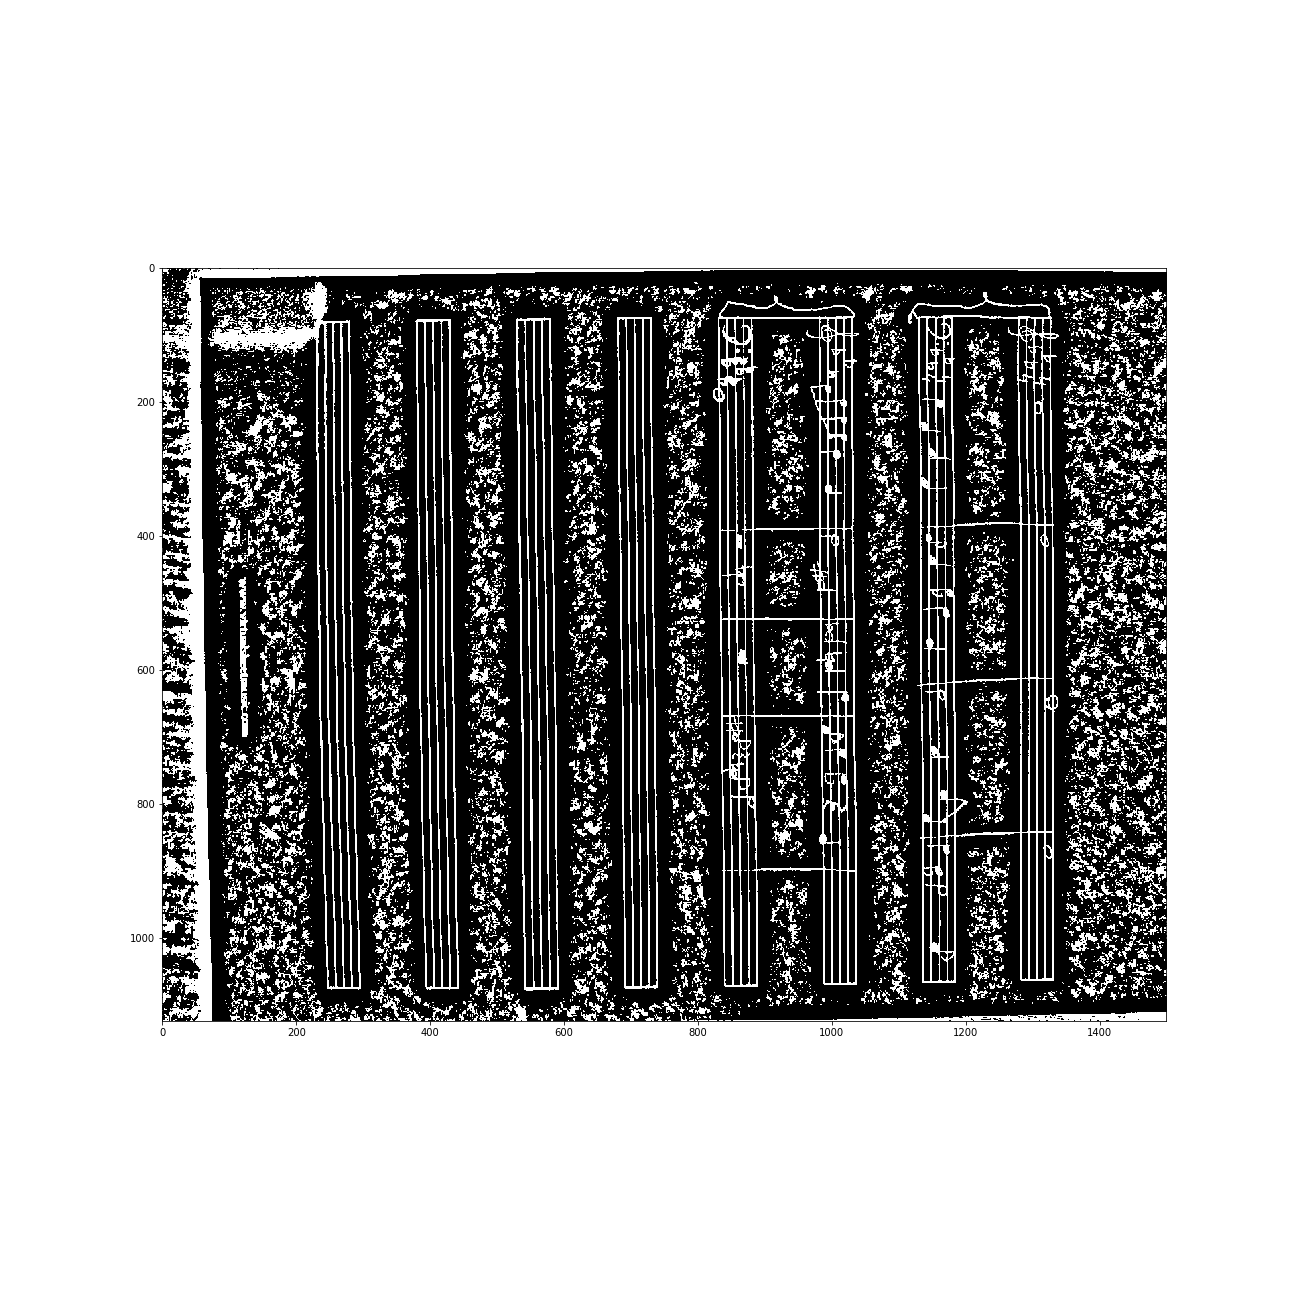
\includegraphics[width=\linewidth]{zdj/Bin0.png}
			\caption{Binaryzacja}
		\end{subfigure}
		\begin{subfigure}[b]{0.32\linewidth}
			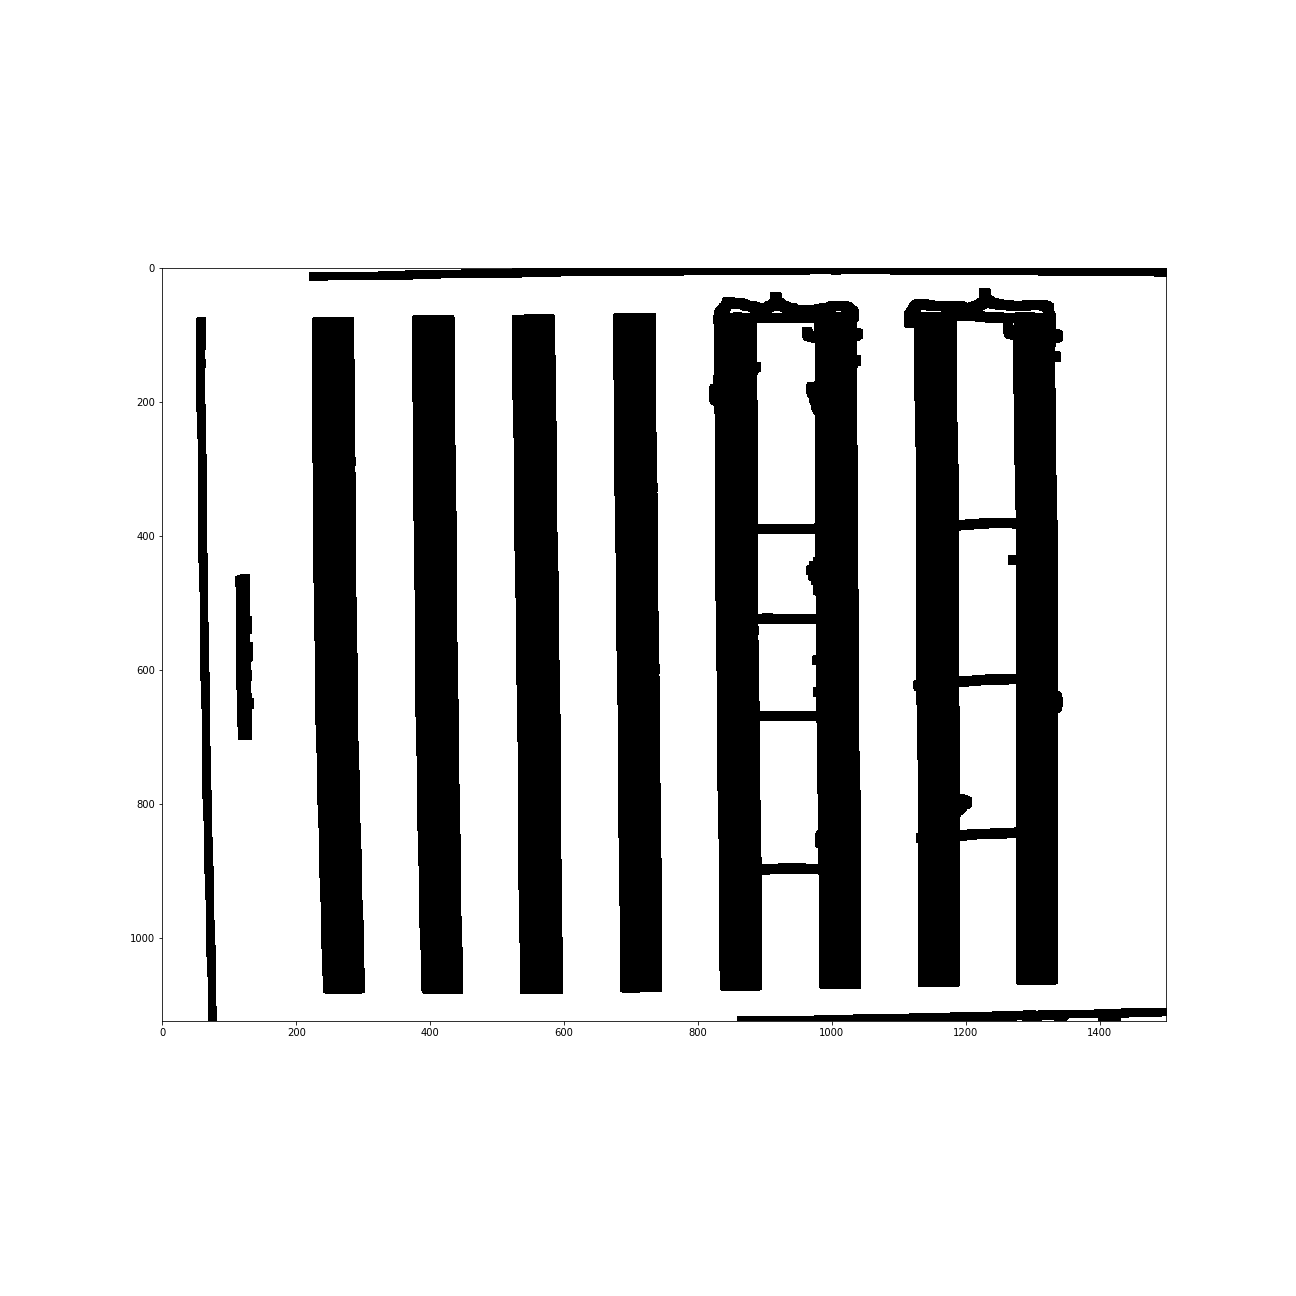
\includegraphics[width=\linewidth]{zdj/Bin1.png}
			\caption{Blob}
		\end{subfigure}
		\begin{subfigure}[b]{0.32\linewidth}
			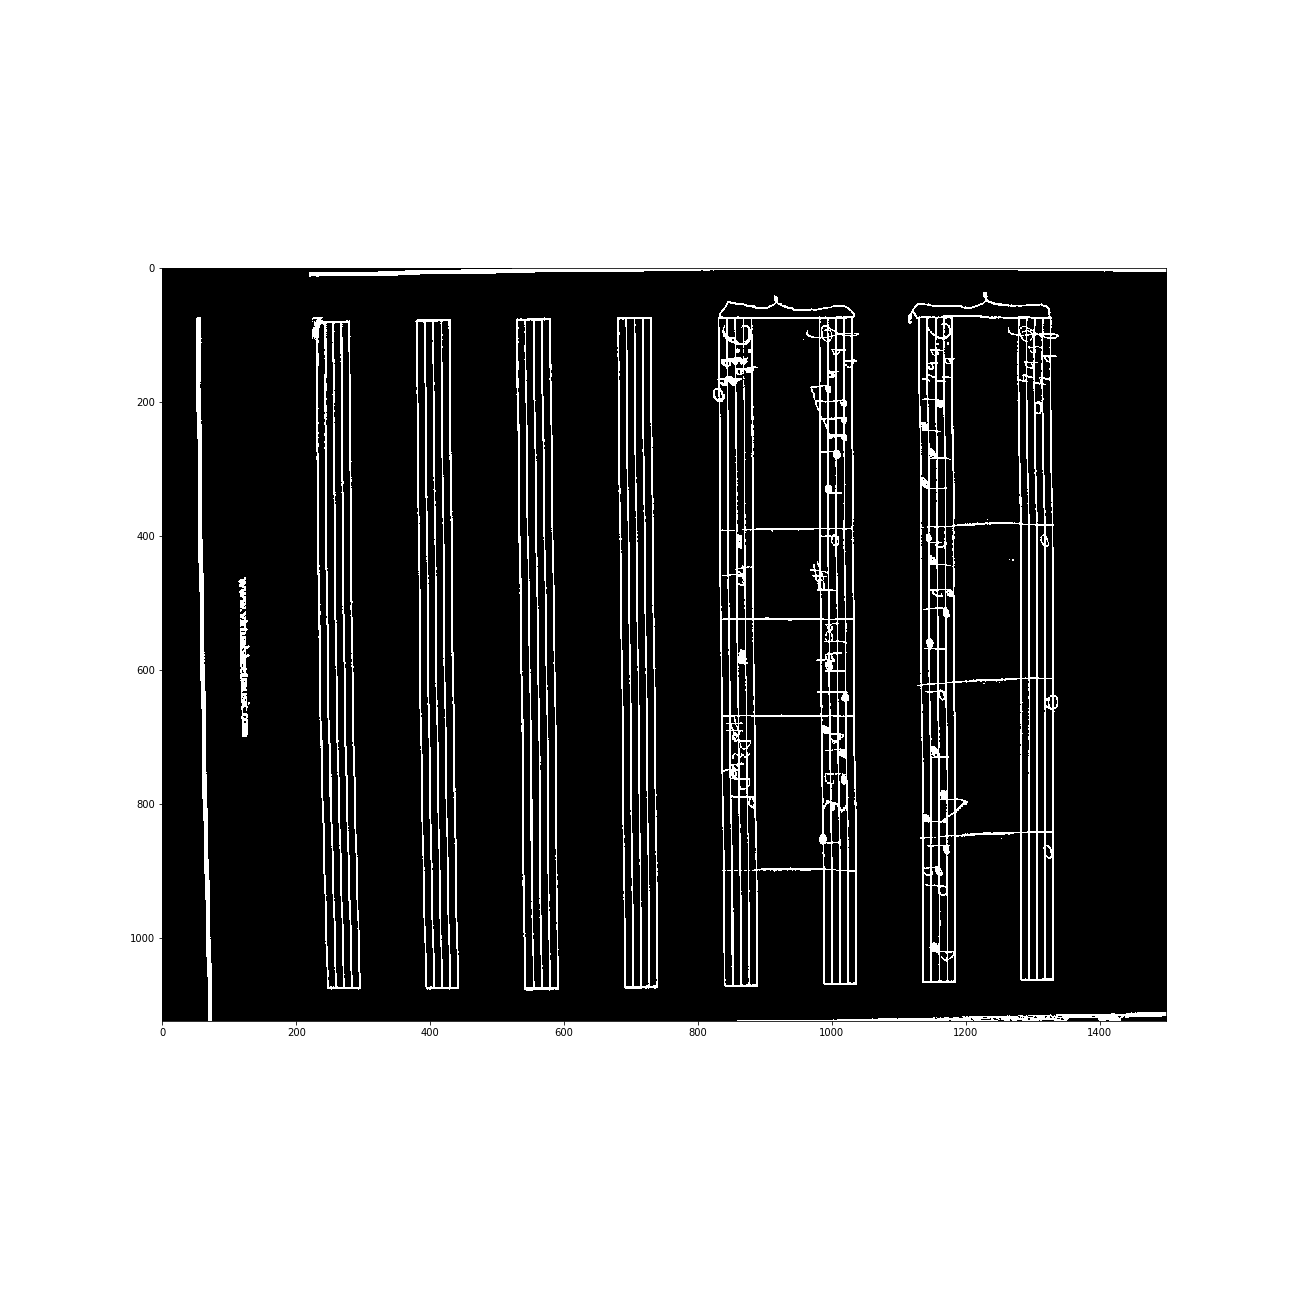
\includegraphics[width=\linewidth]{zdj/Bin2.png}
			\caption{Oczyszczona binaryzacja}
		\end{subfigure}
		\caption{Proces Binaryzacji.}
		\label{fig:binary}
	\end{figure}

	\begin{figure}[h!]
		\centering
		\begin{subfigure}[b]{0.48\linewidth}
			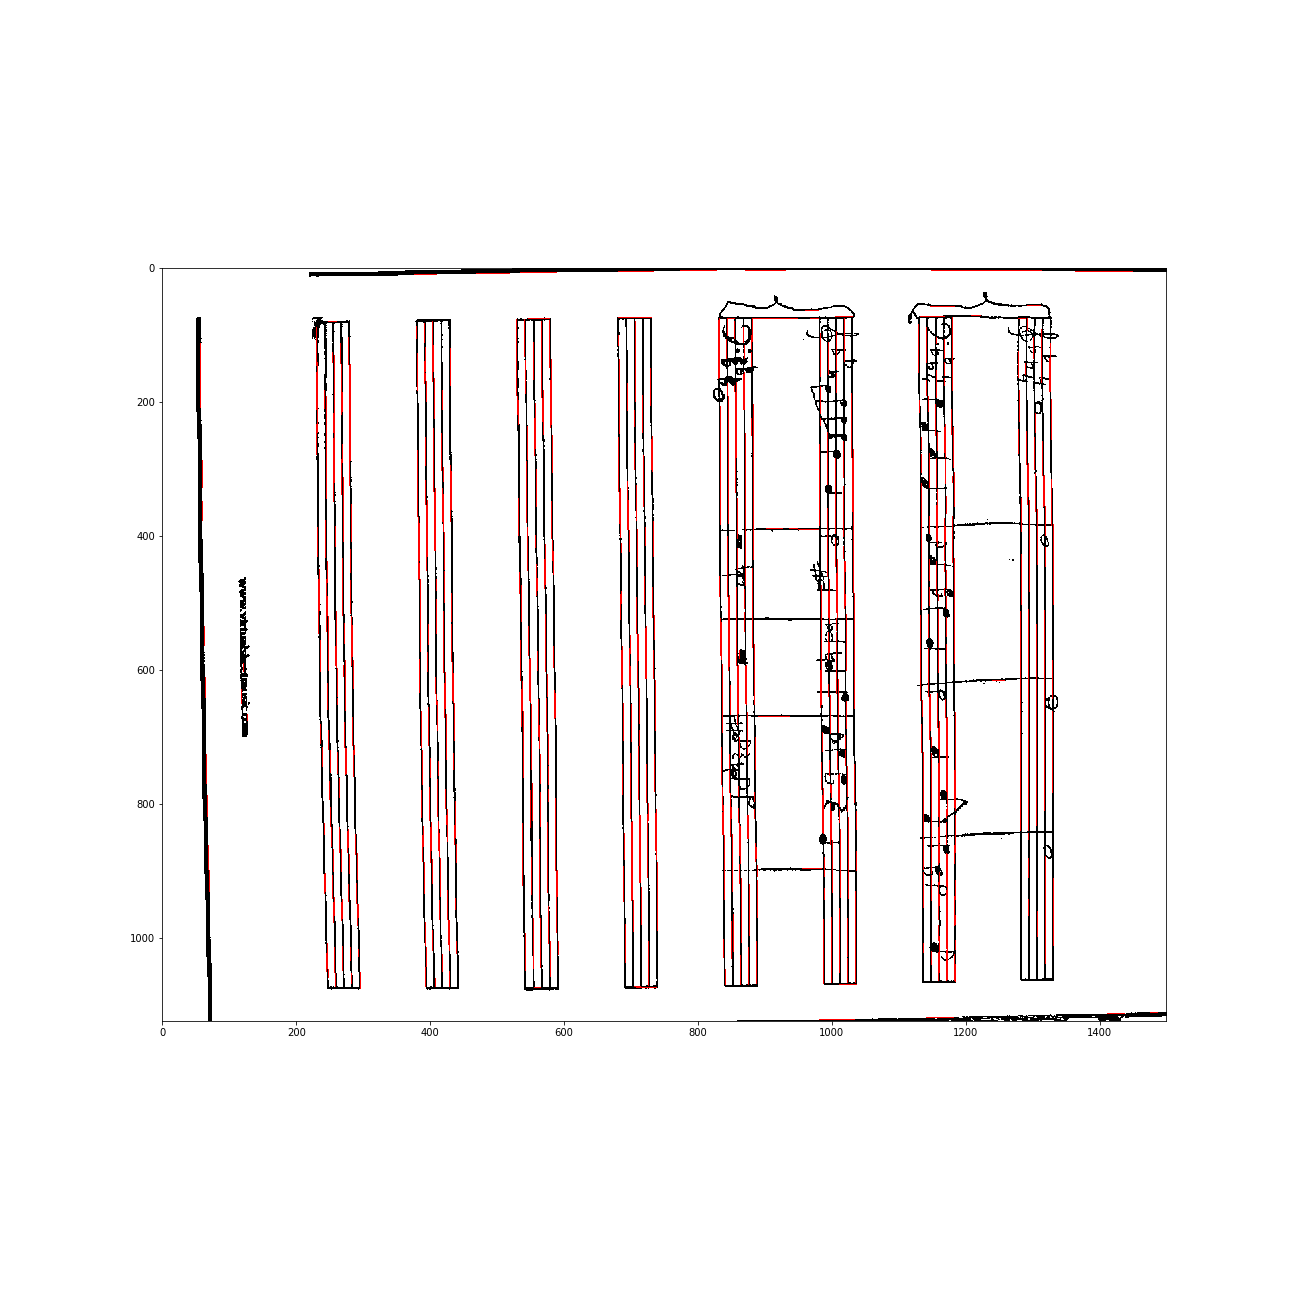
\includegraphics[width=\linewidth]{zdj/Rot0.png}
			\caption{Linie proste}
		\end{subfigure}
		\begin{subfigure}[b]{0.48\linewidth}
			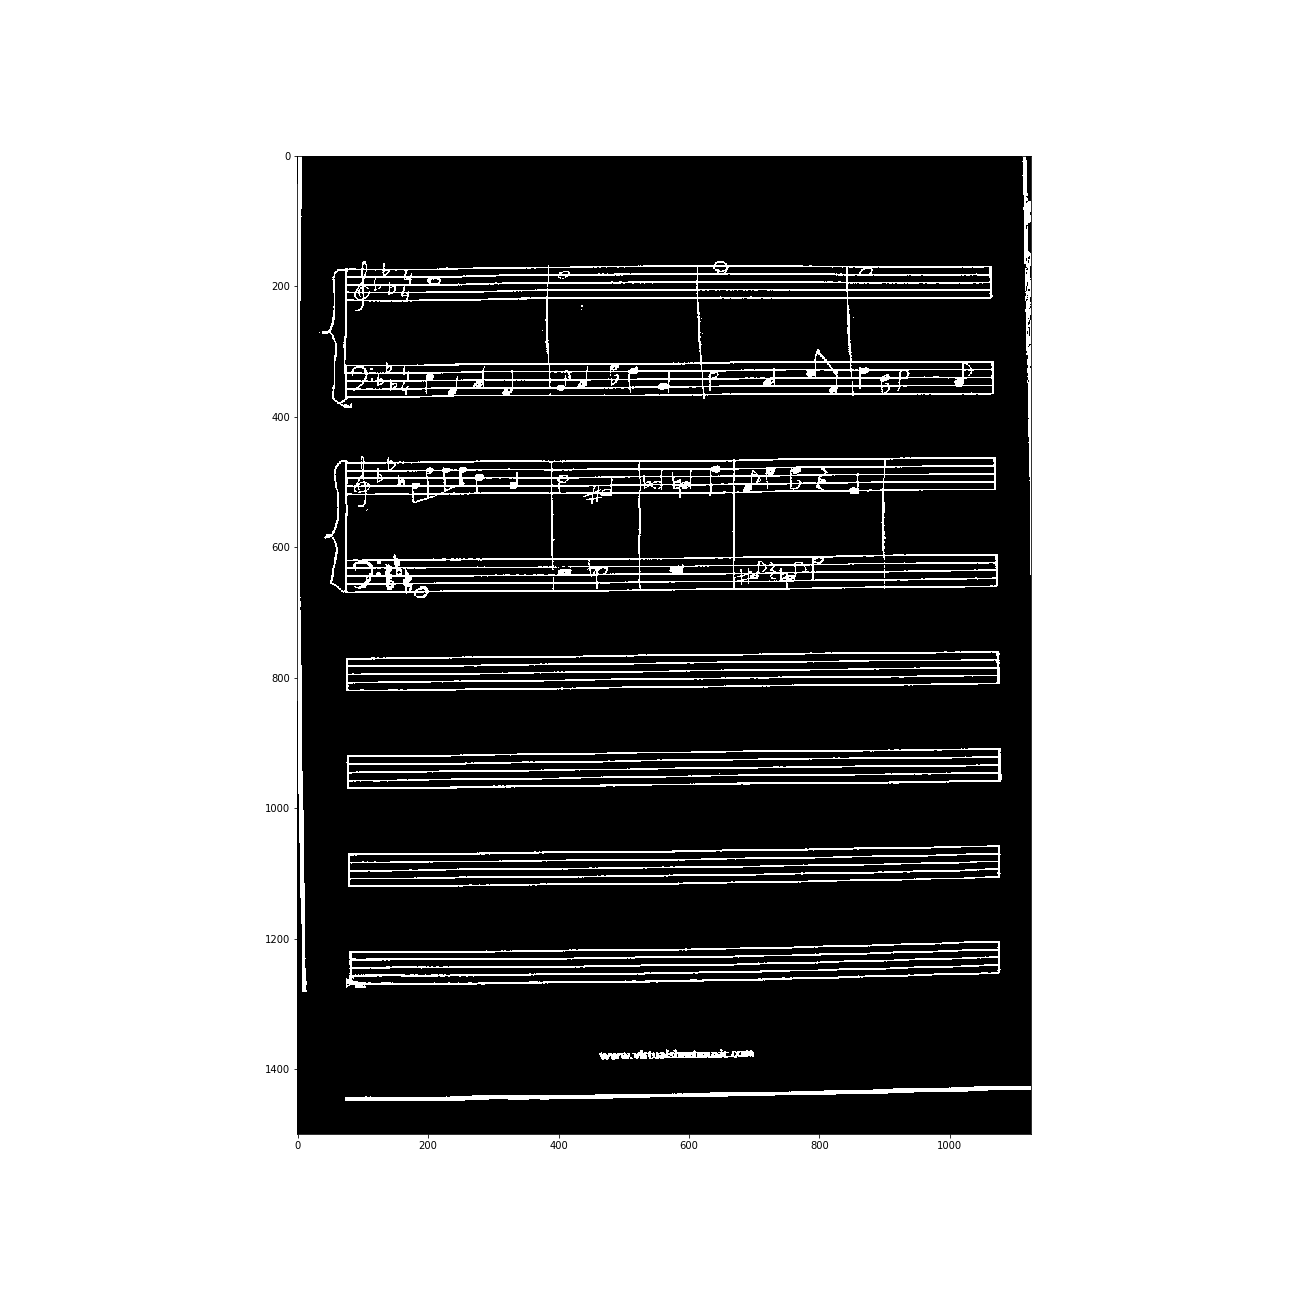
\includegraphics[width=\linewidth]{zdj/Rot1.png}
			\caption{Obrót}
		\end{subfigure}
		\caption{Proces Rotacji.}
		\label{fig:rotate}
	\end{figure}

	\begin{figure}[h!]
		\begin{subfigure}[b]{0.32\linewidth}
			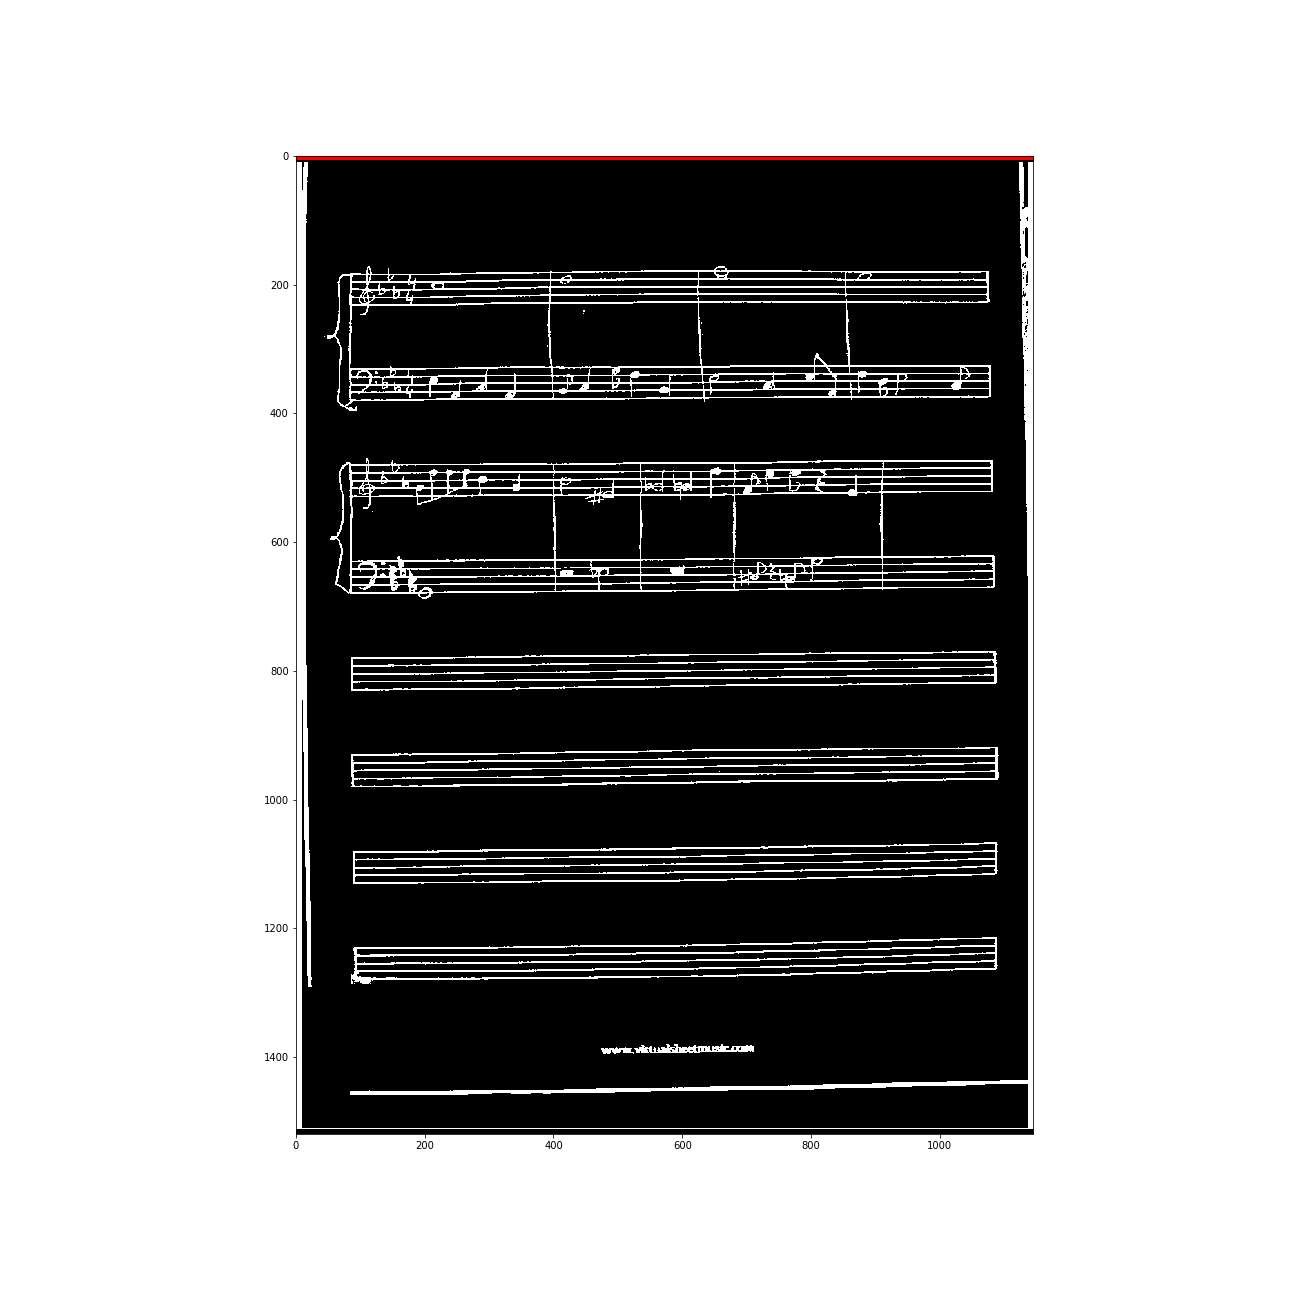
\includegraphics[width=\linewidth]{zdj/BFS0.png}
		\end{subfigure}
		\begin{subfigure}[b]{0.32\linewidth}
			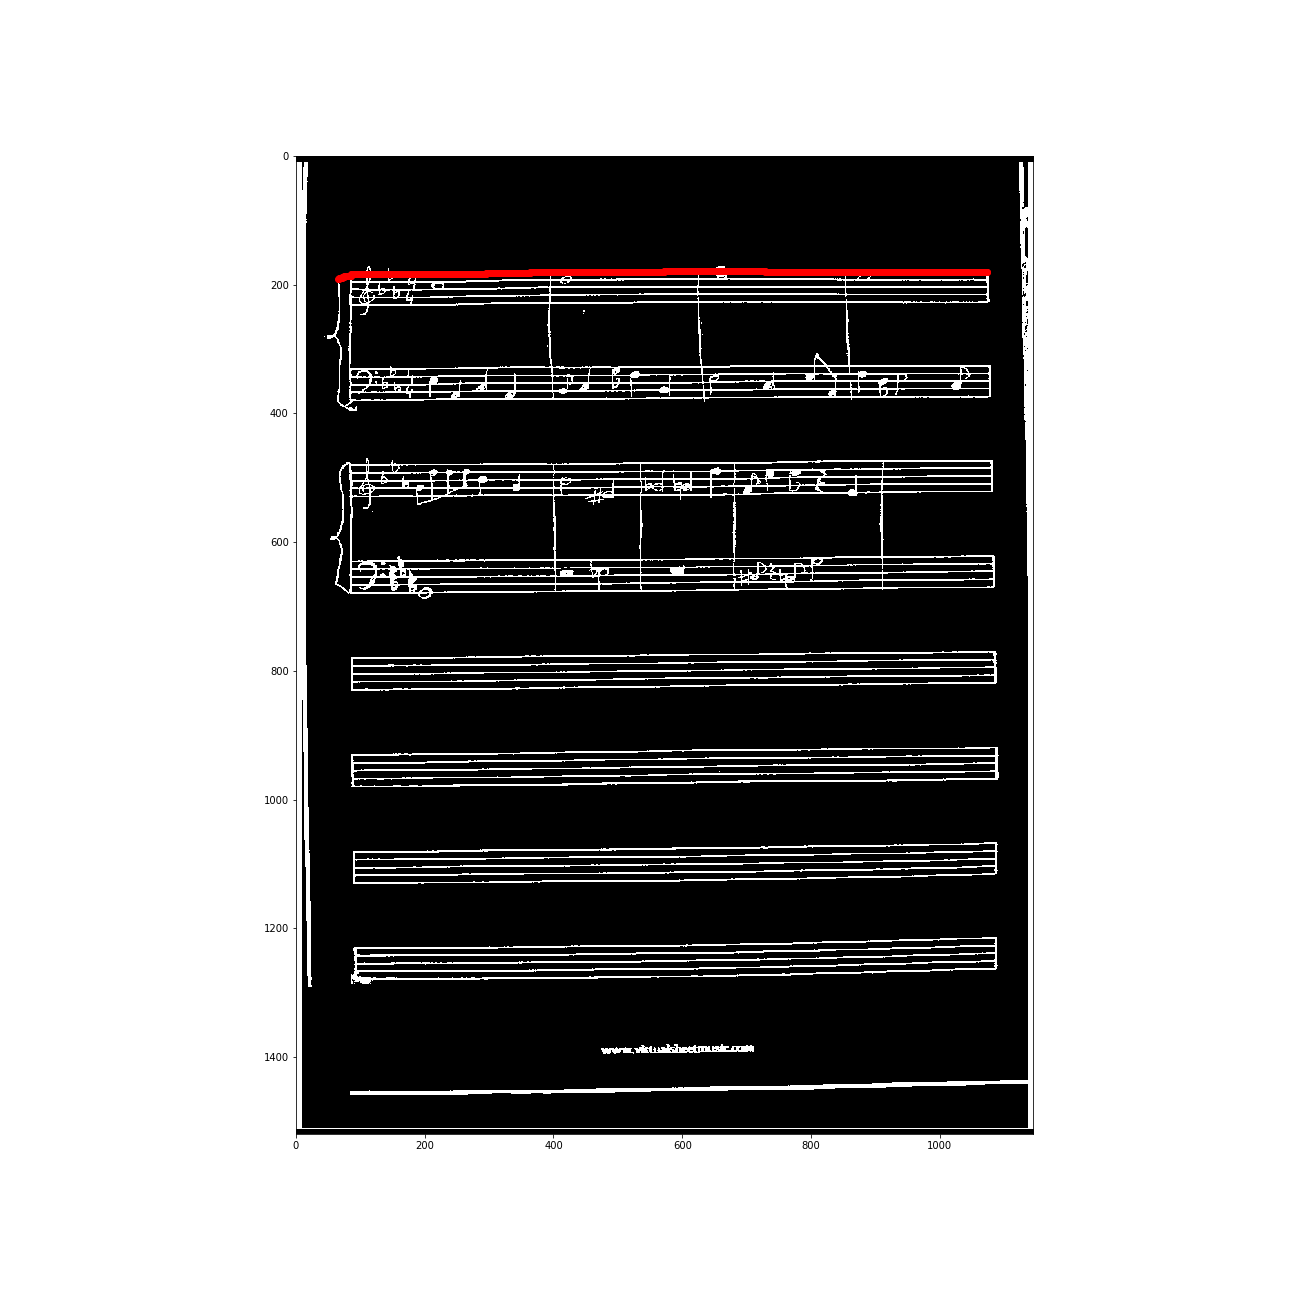
\includegraphics[width=\linewidth]{zdj/BFS1.png}
		\end{subfigure}
		\begin{subfigure}[b]{0.32\linewidth}
			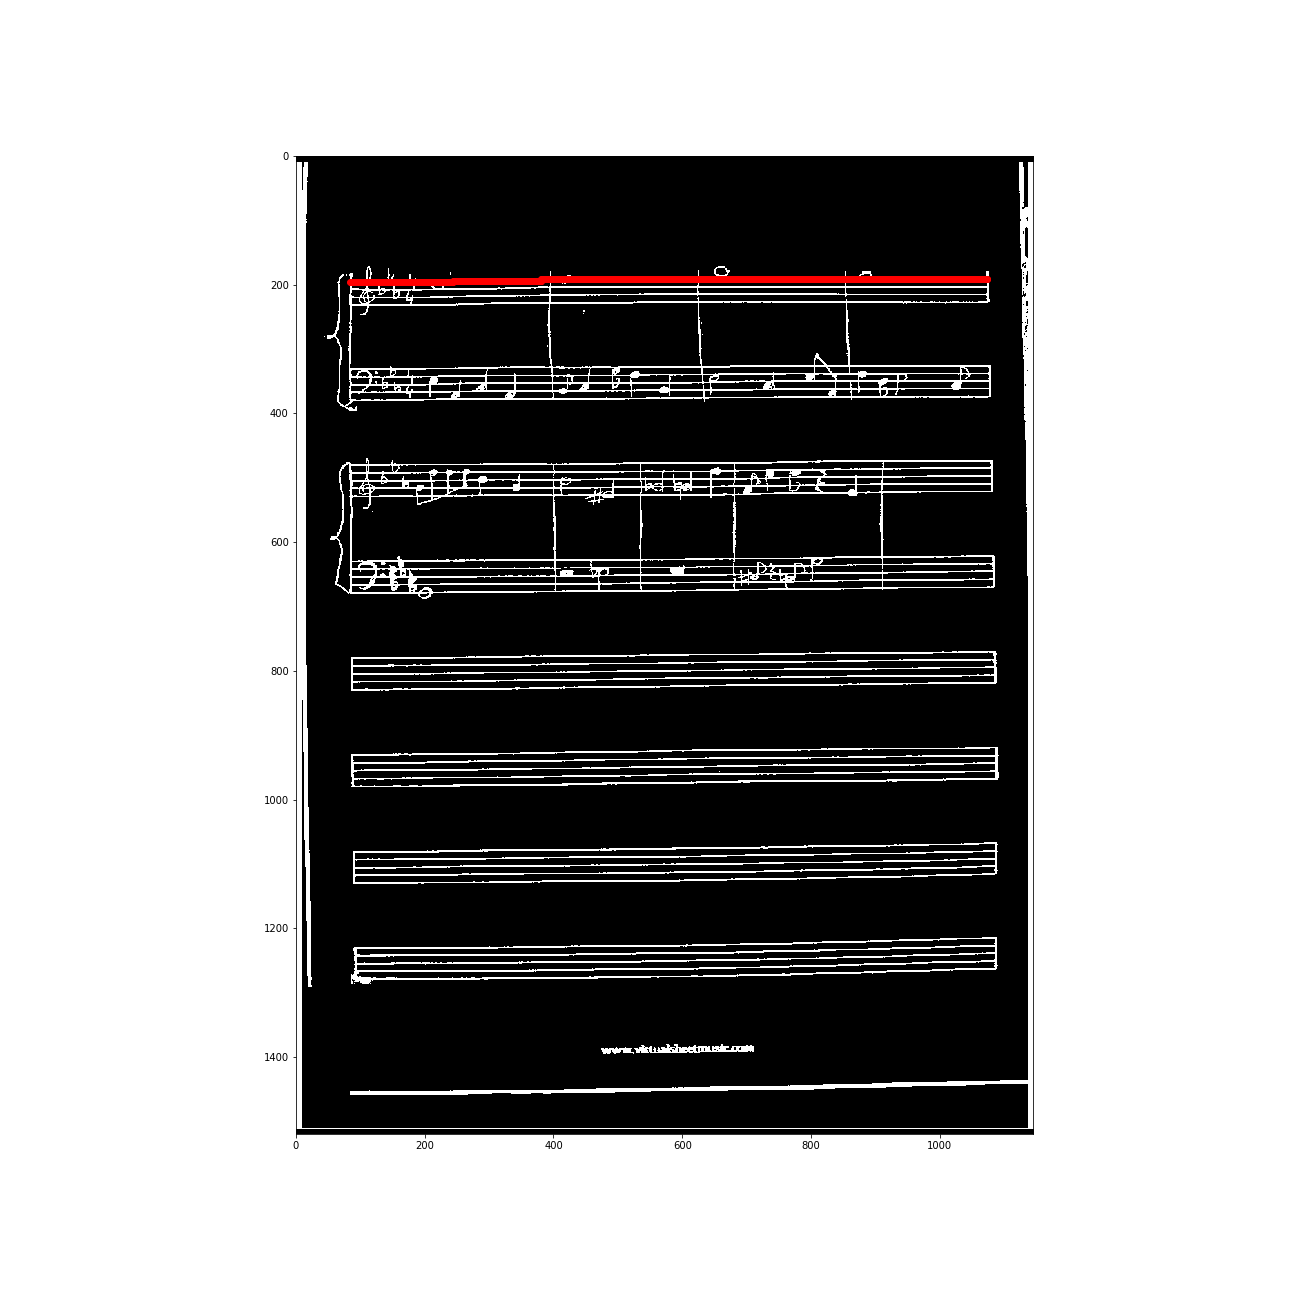
\includegraphics[width=\linewidth]{zdj/BFS2.png}
		\end{subfigure}
		\begin{subfigure}[b]{0.32\linewidth}
			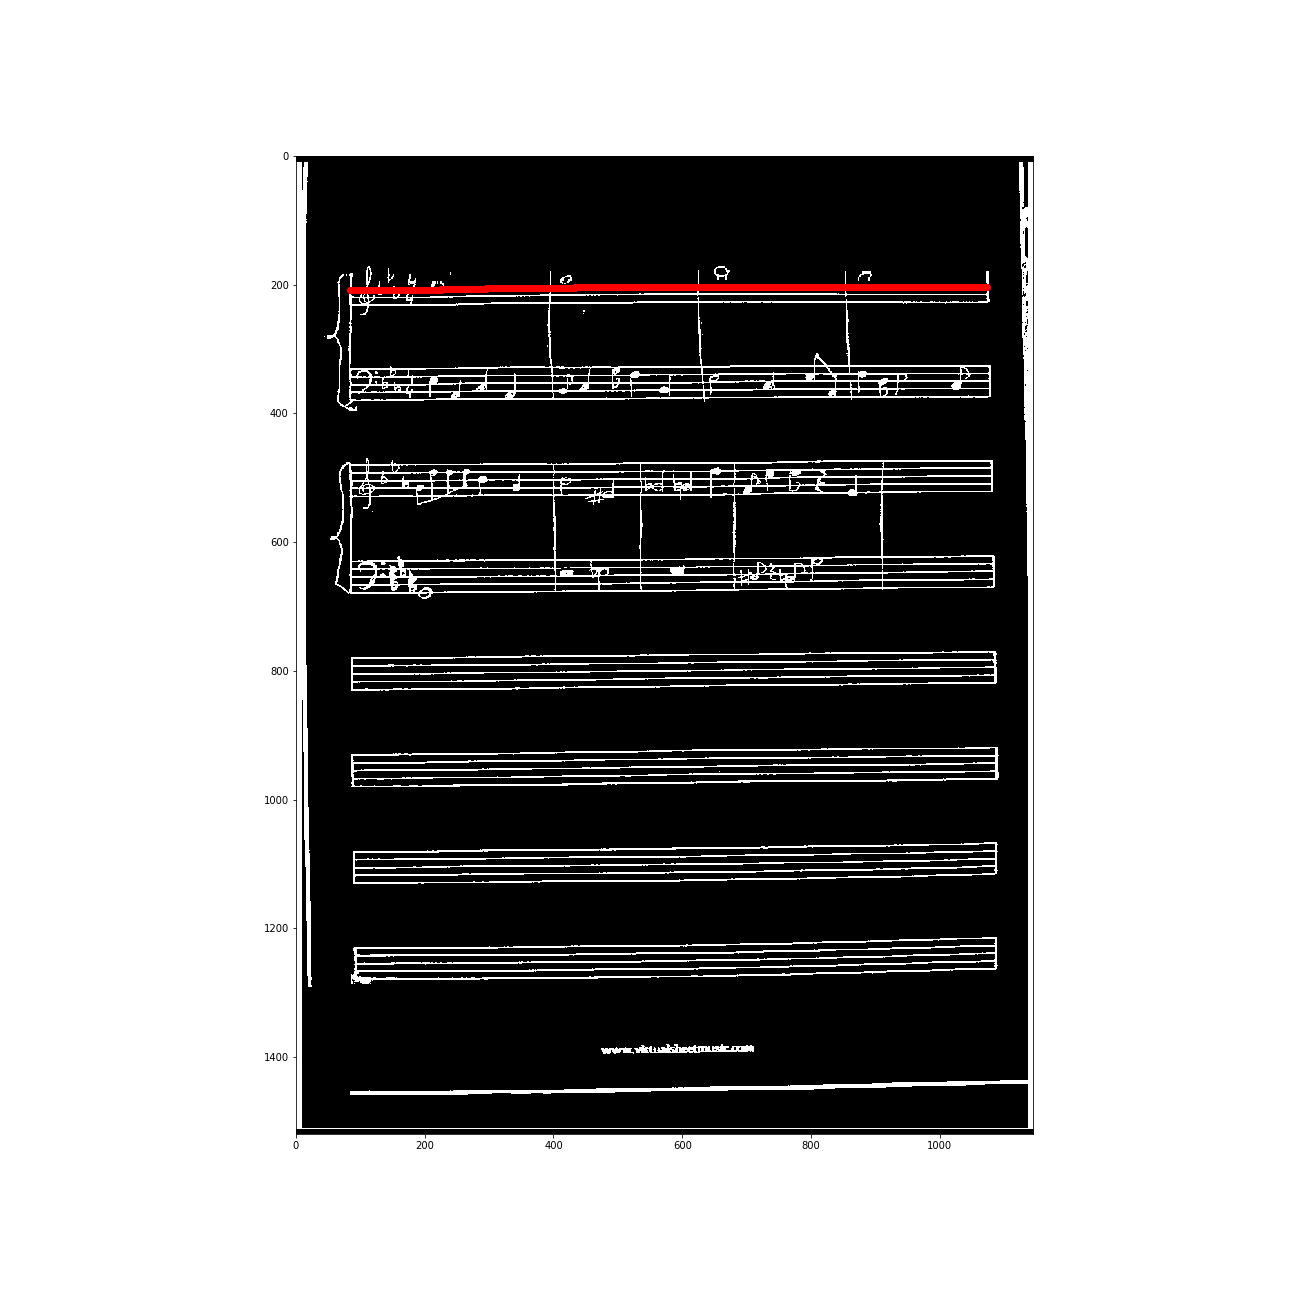
\includegraphics[width=\linewidth]{zdj/BFS3.png}
		\end{subfigure}
		\begin{subfigure}[b]{0.32\linewidth}
			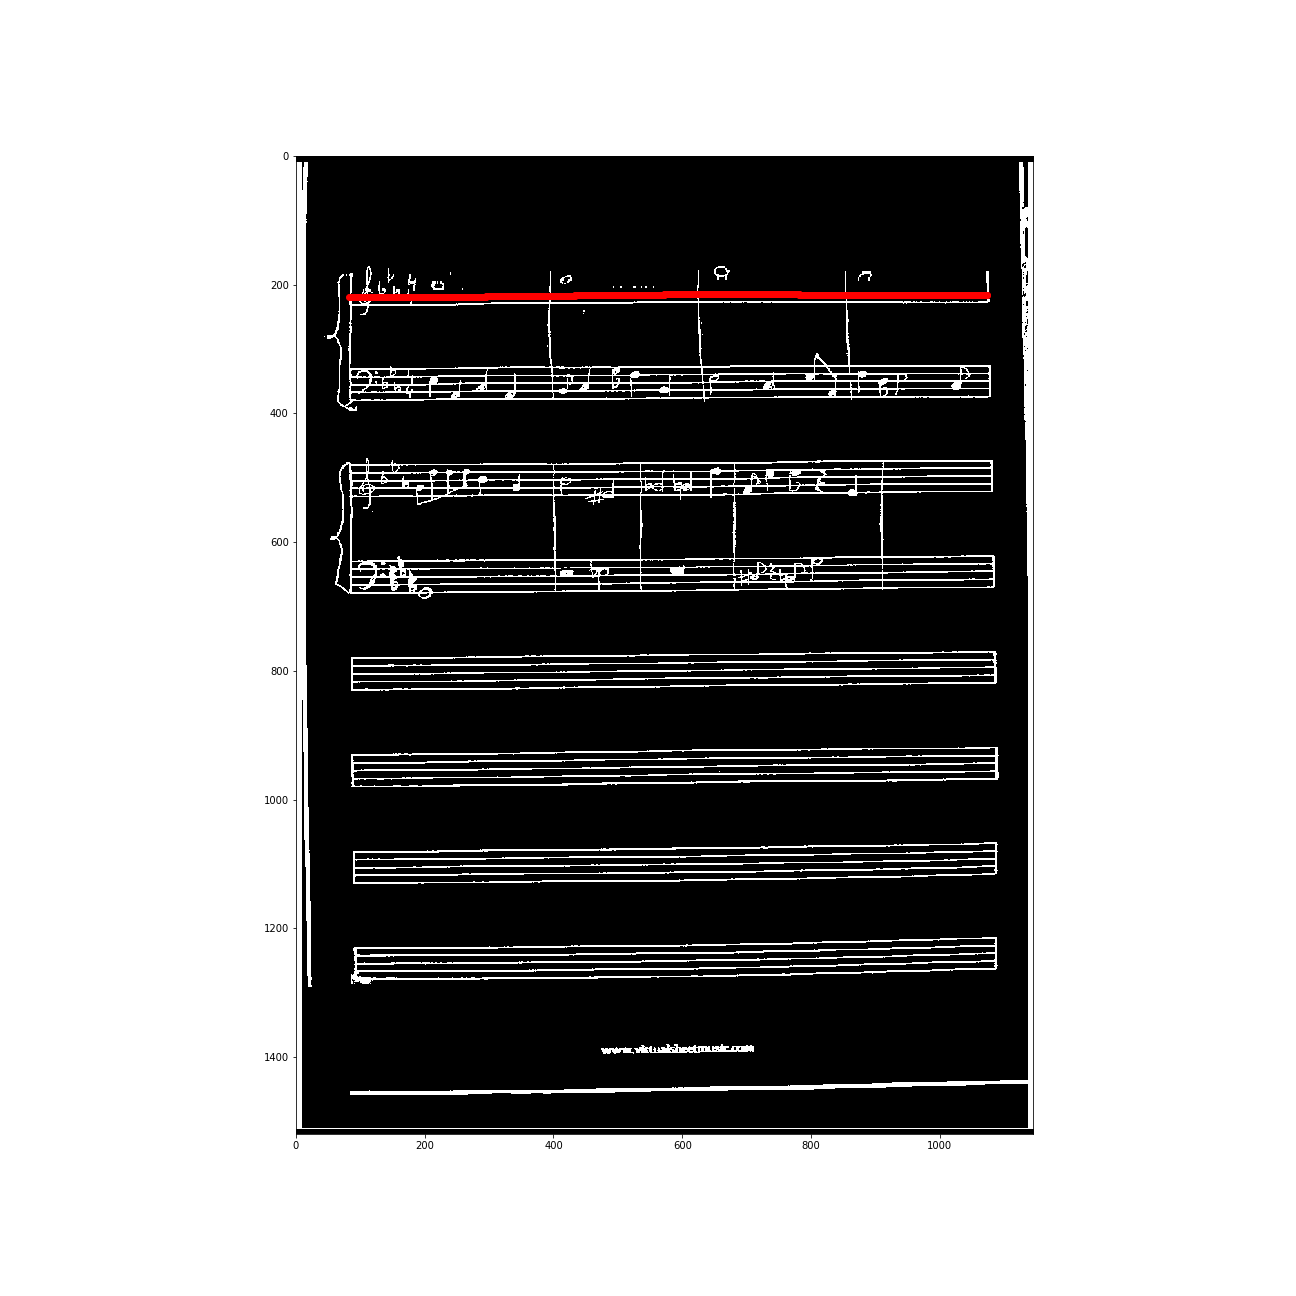
\includegraphics[width=\linewidth]{zdj/BFS4.png}
		\end{subfigure}
		\begin{subfigure}[b]{0.32\linewidth}
			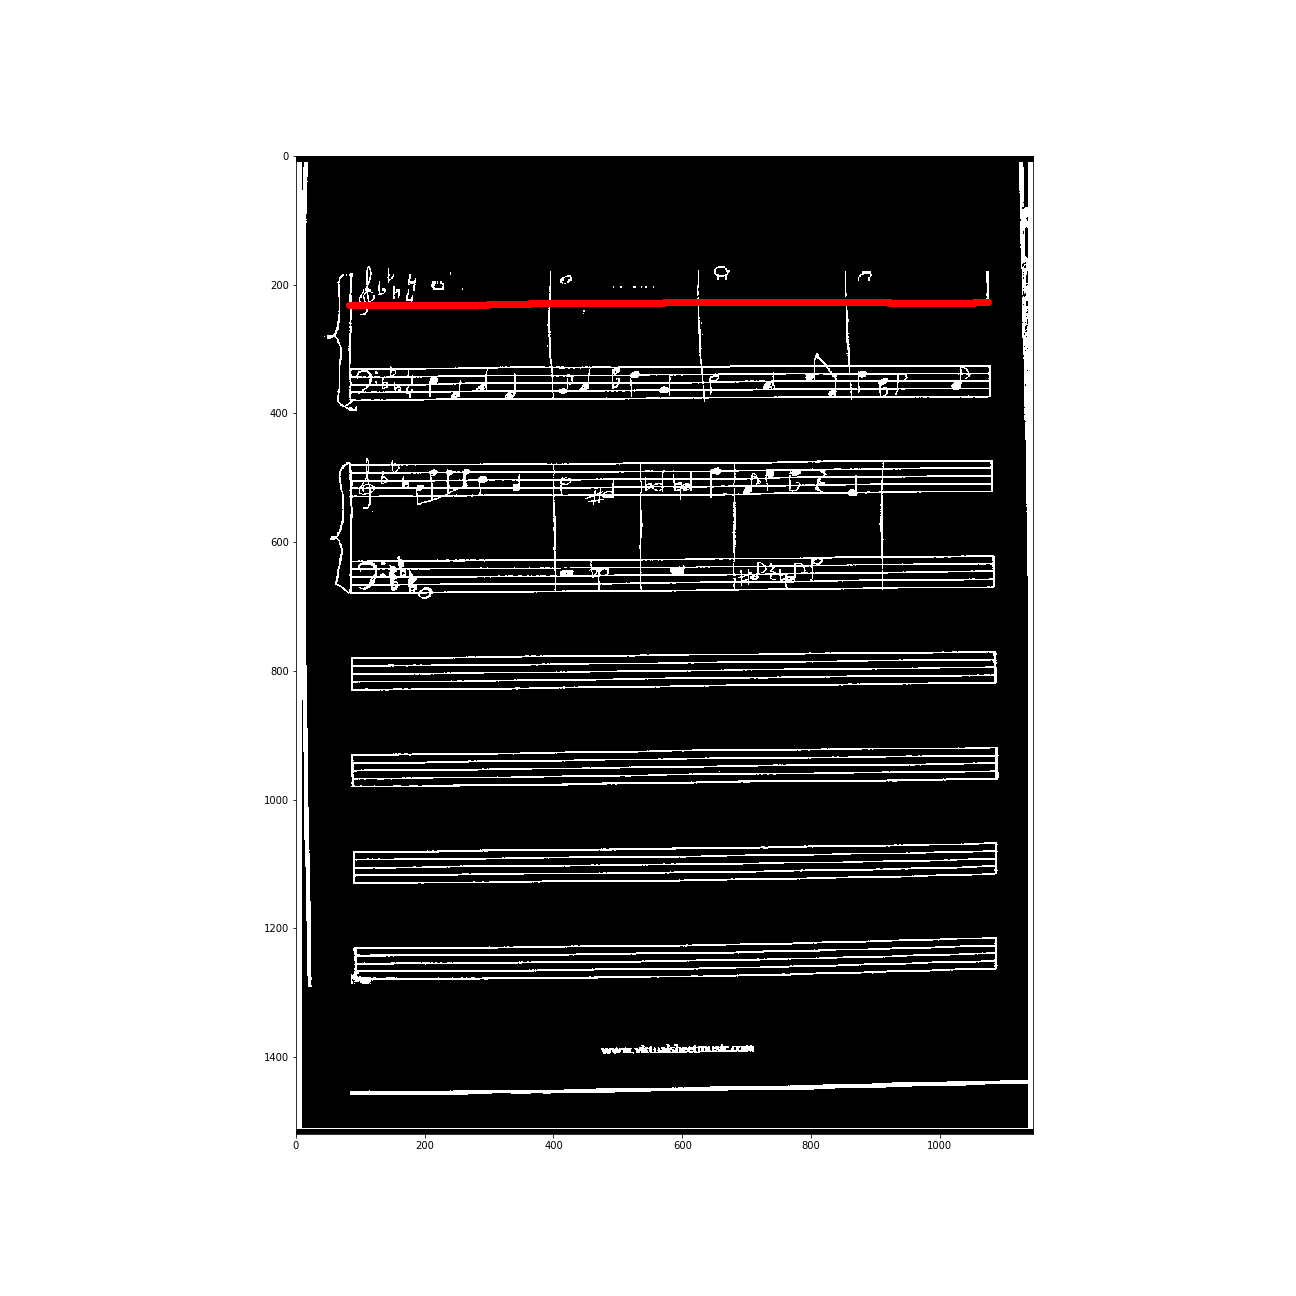
\includegraphics[width=\linewidth]{zdj/BFS5.png}
		\end{subfigure}
		\begin{subfigure}[b]{0.32\linewidth}
			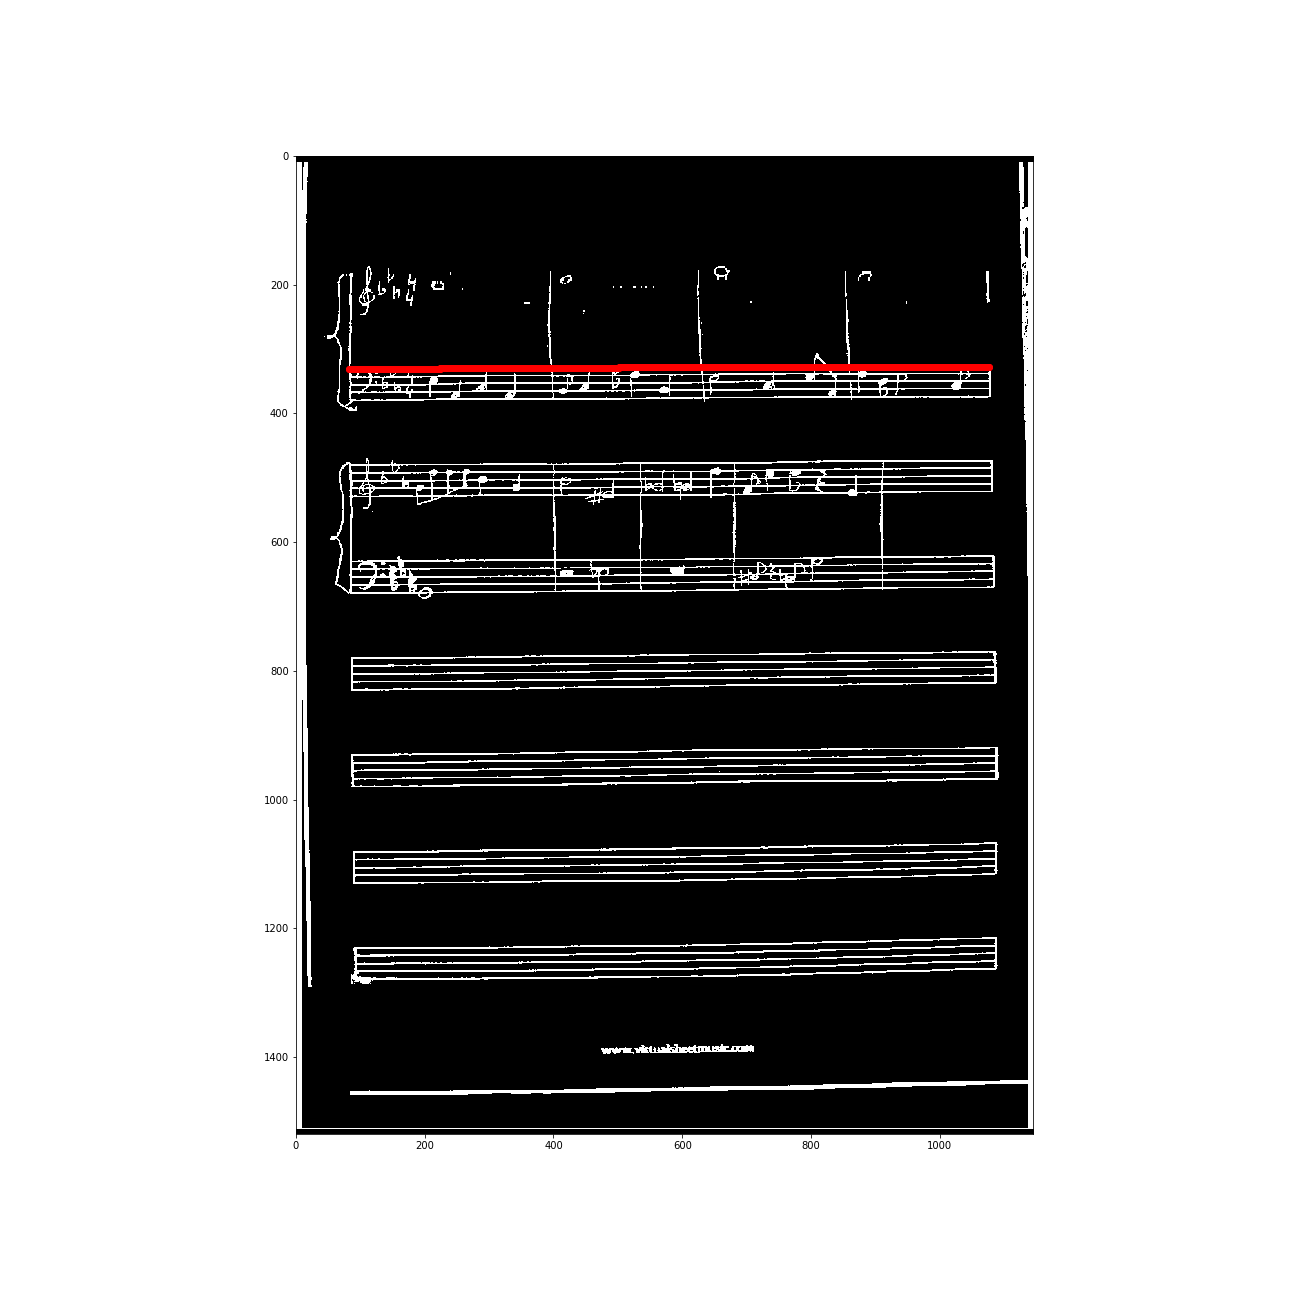
\includegraphics[width=\linewidth]{zdj/BFS6.png}
		\end{subfigure}
		\begin{subfigure}[b]{0.32\linewidth}
			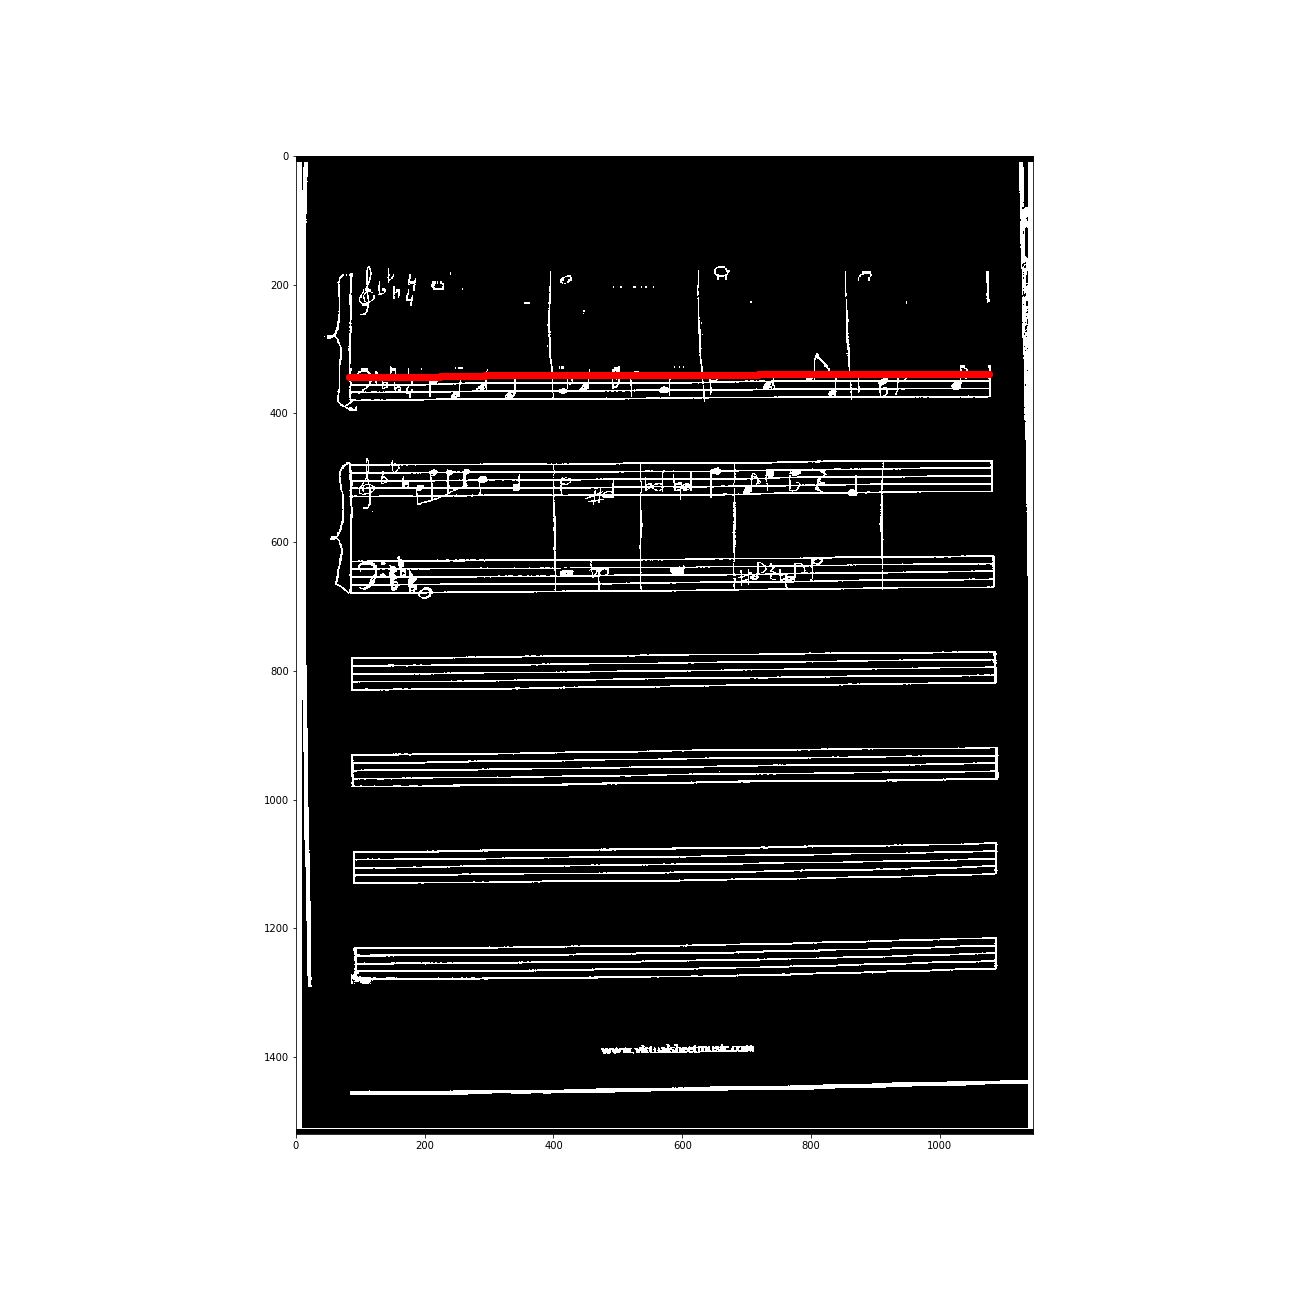
\includegraphics[width=\linewidth]{zdj/BFS7.png}
		\end{subfigure}
		\begin{subfigure}[b]{0.32\linewidth}
			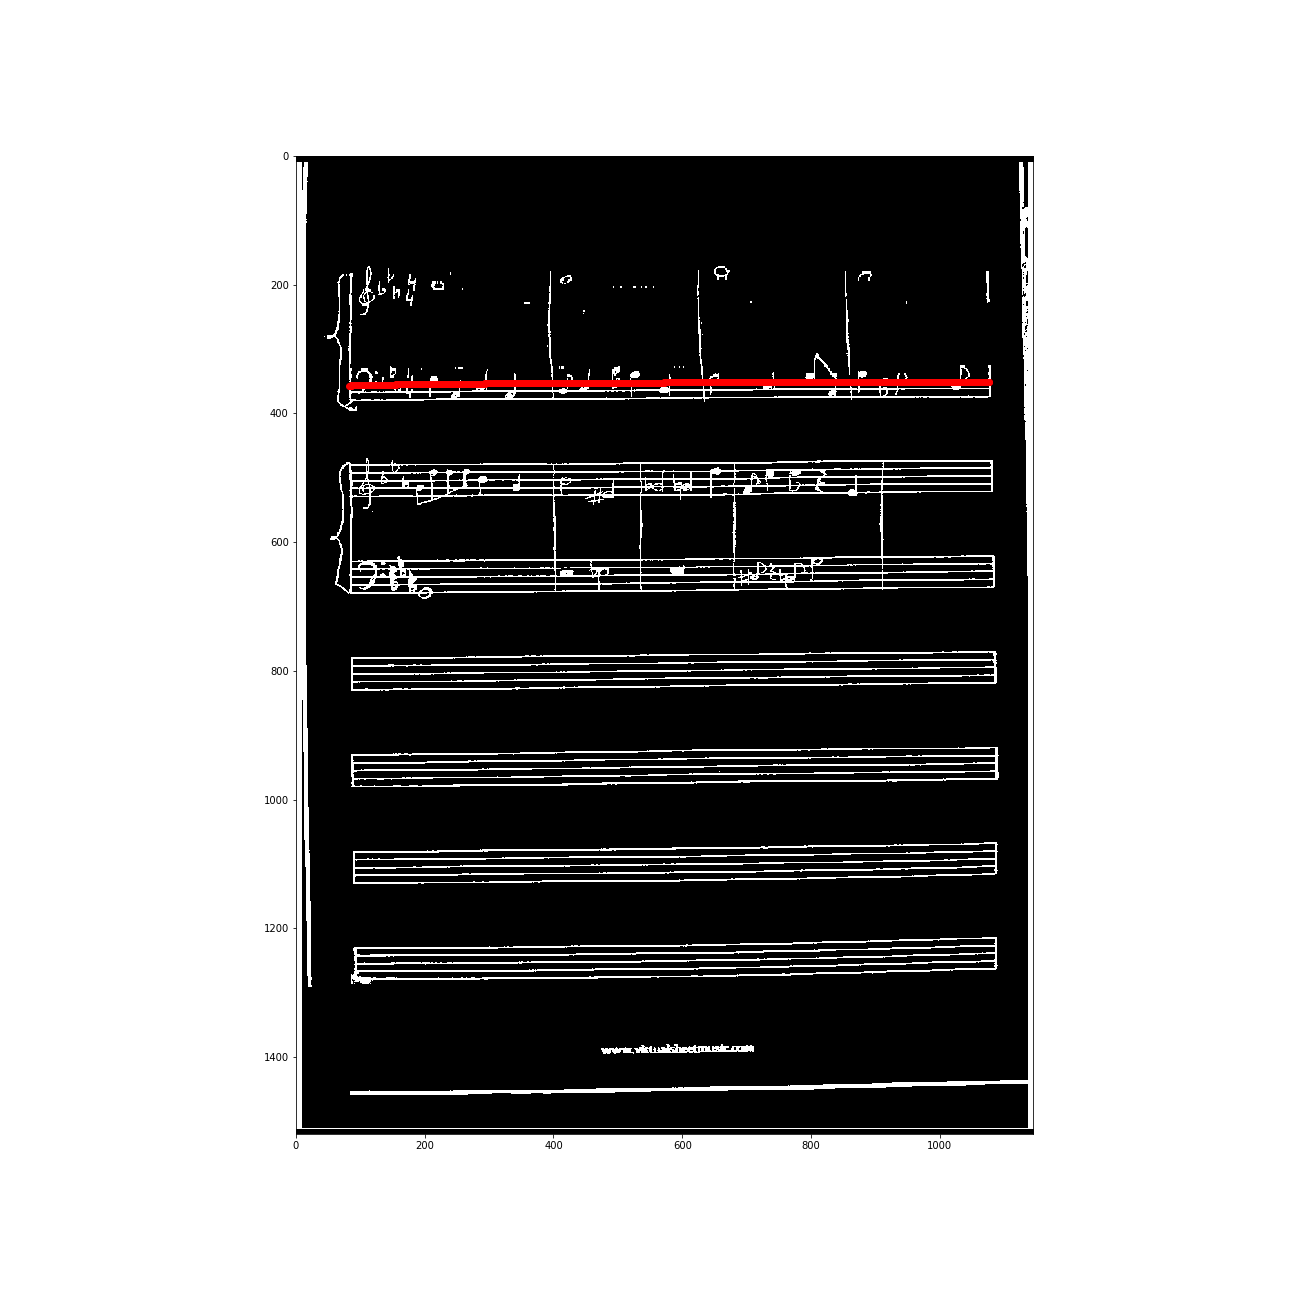
\includegraphics[width=\linewidth]{zdj/BFS8.png}
		\end{subfigure}
		\begin{subfigure}[b]{0.32\linewidth}
			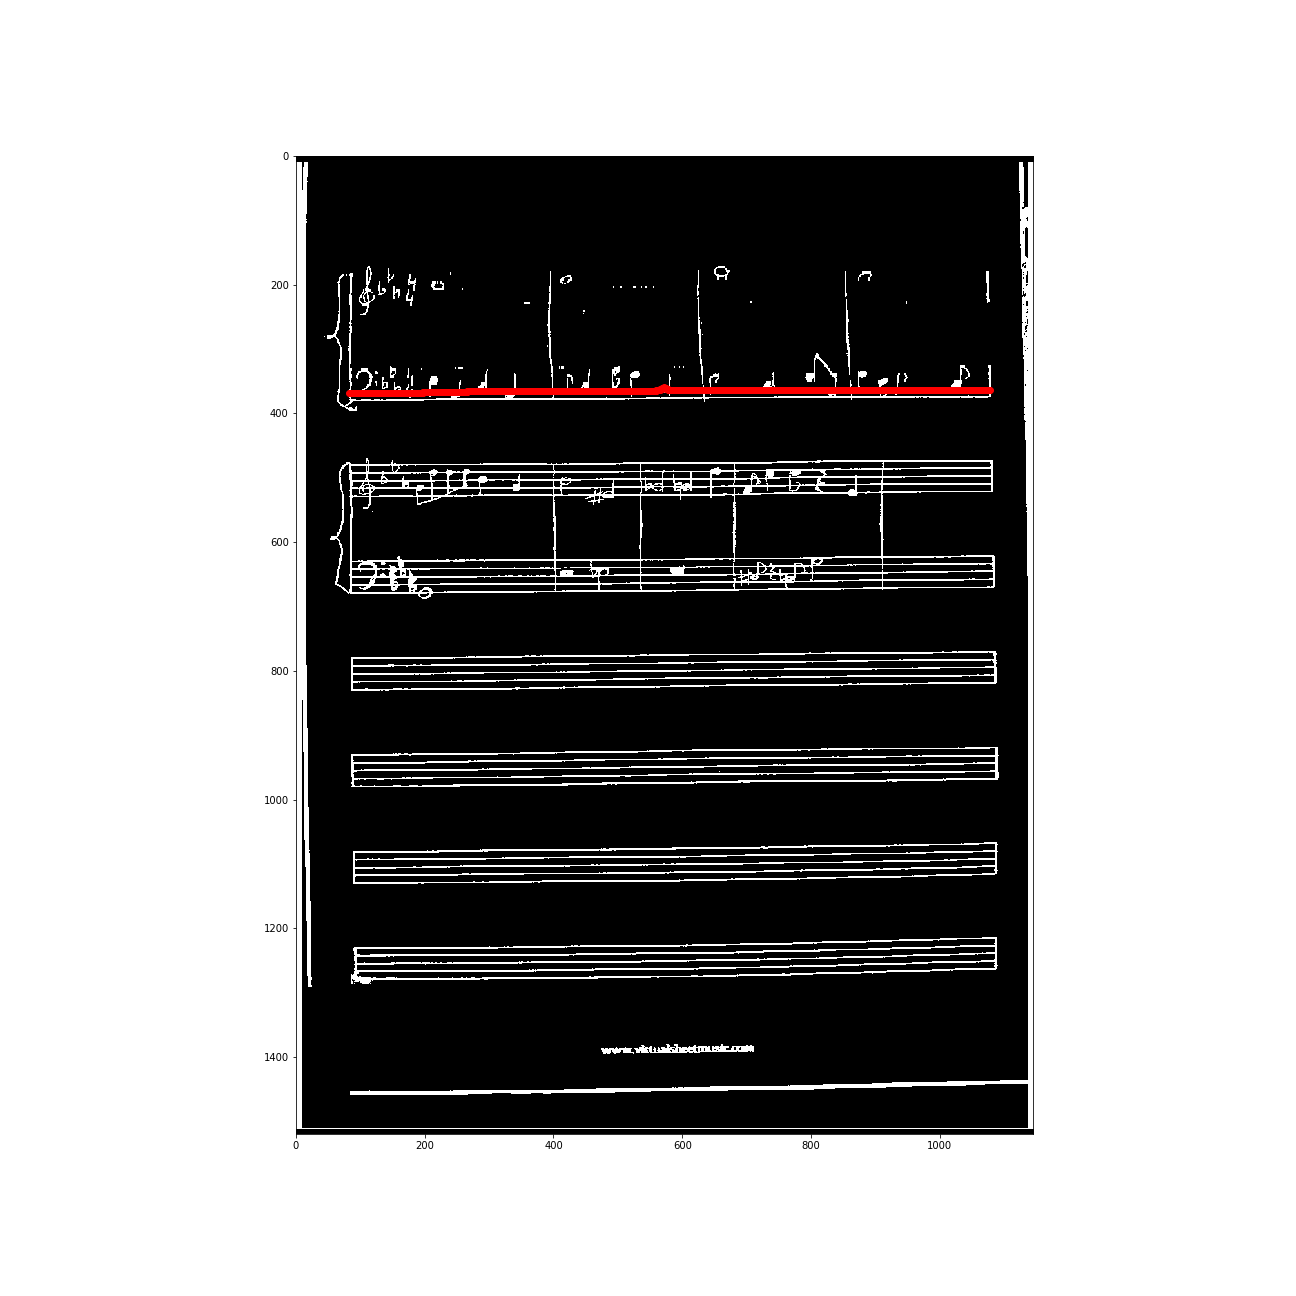
\includegraphics[width=\linewidth]{zdj/BFS9.png}
		\end{subfigure}
		\begin{subfigure}[b]{0.32\linewidth}
			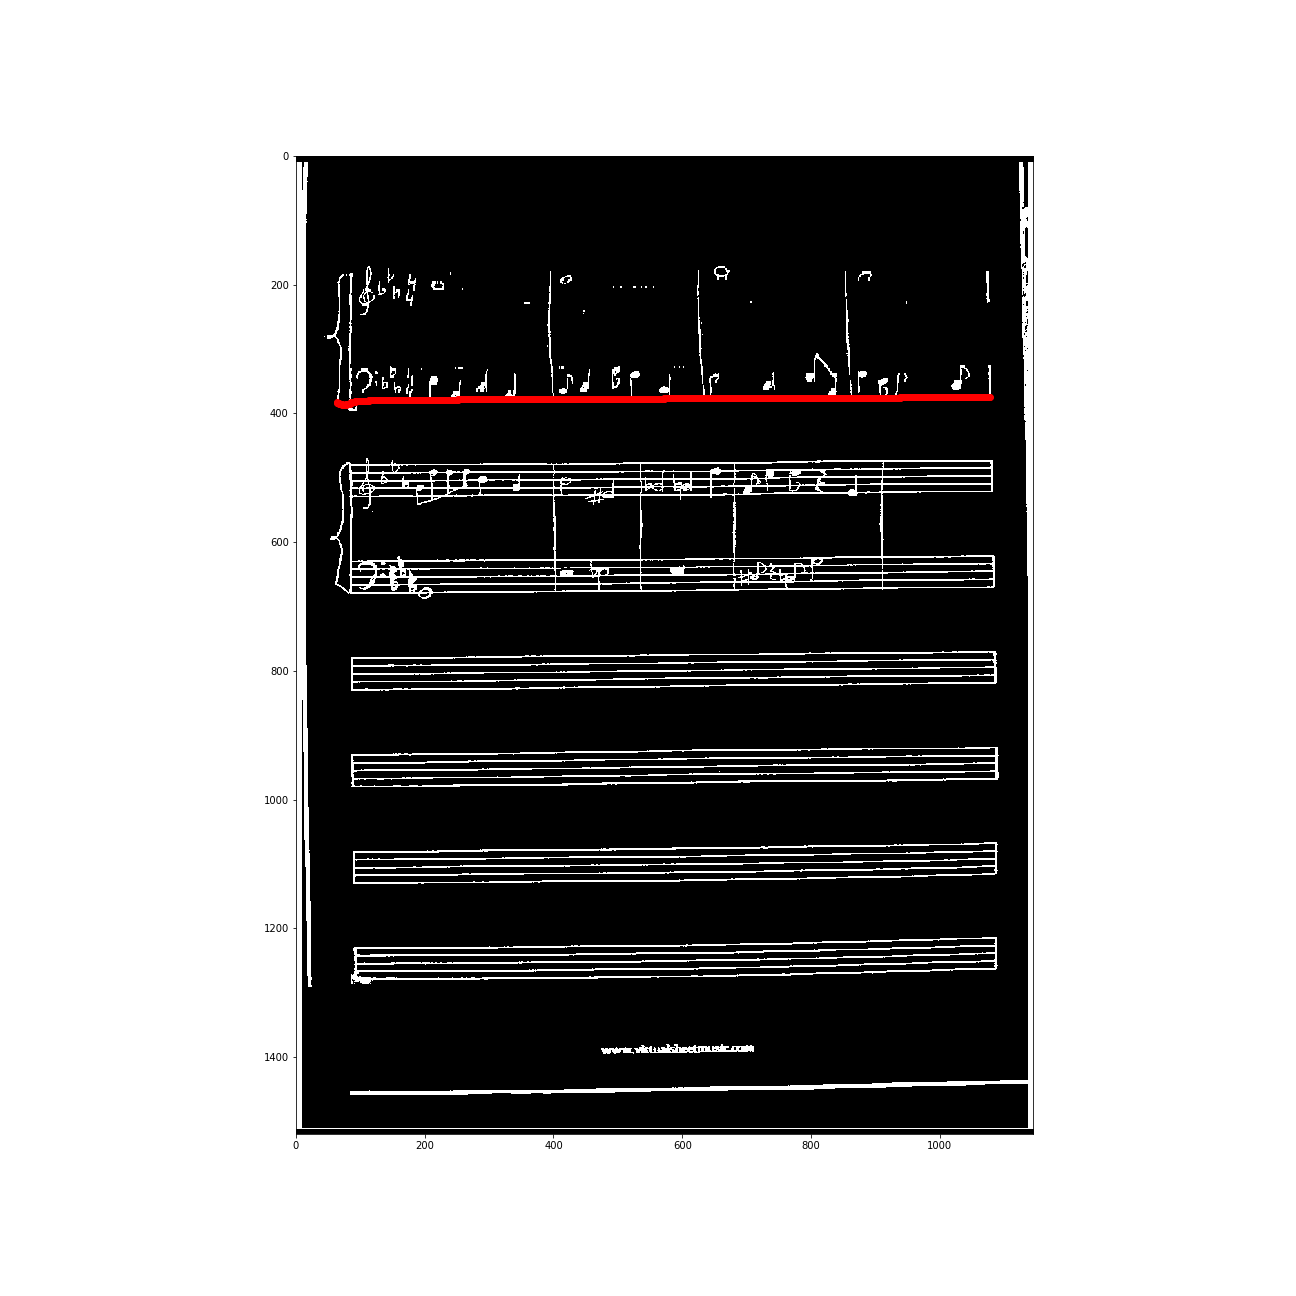
\includegraphics[width=\linewidth]{zdj/BFS10.png}
		\end{subfigure}
		\begin{subfigure}[b]{0.32\linewidth}
			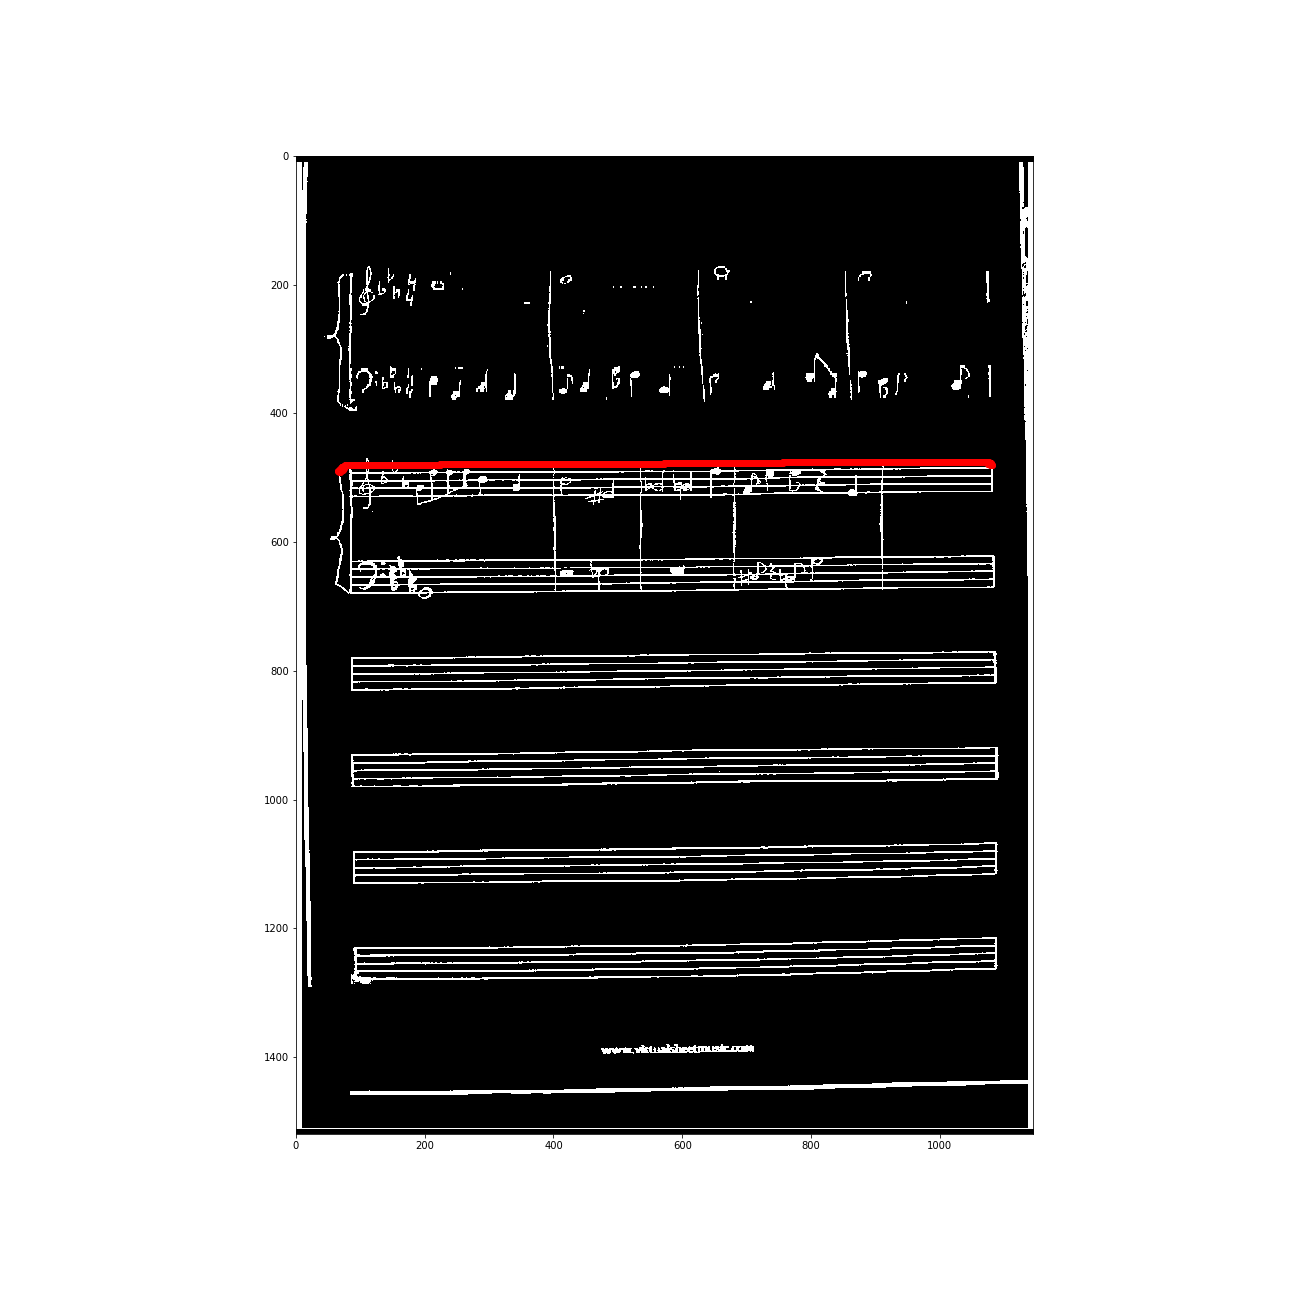
\includegraphics[width=\linewidth]{zdj/BFS11.png}
		\end{subfigure}
		\caption{Proces Detekcji i usuwania linii 1.}
		\label{fig:bfs1}
	\end{figure}

	\begin{figure}[h!]
		\begin{subfigure}[b]{0.32\linewidth}
			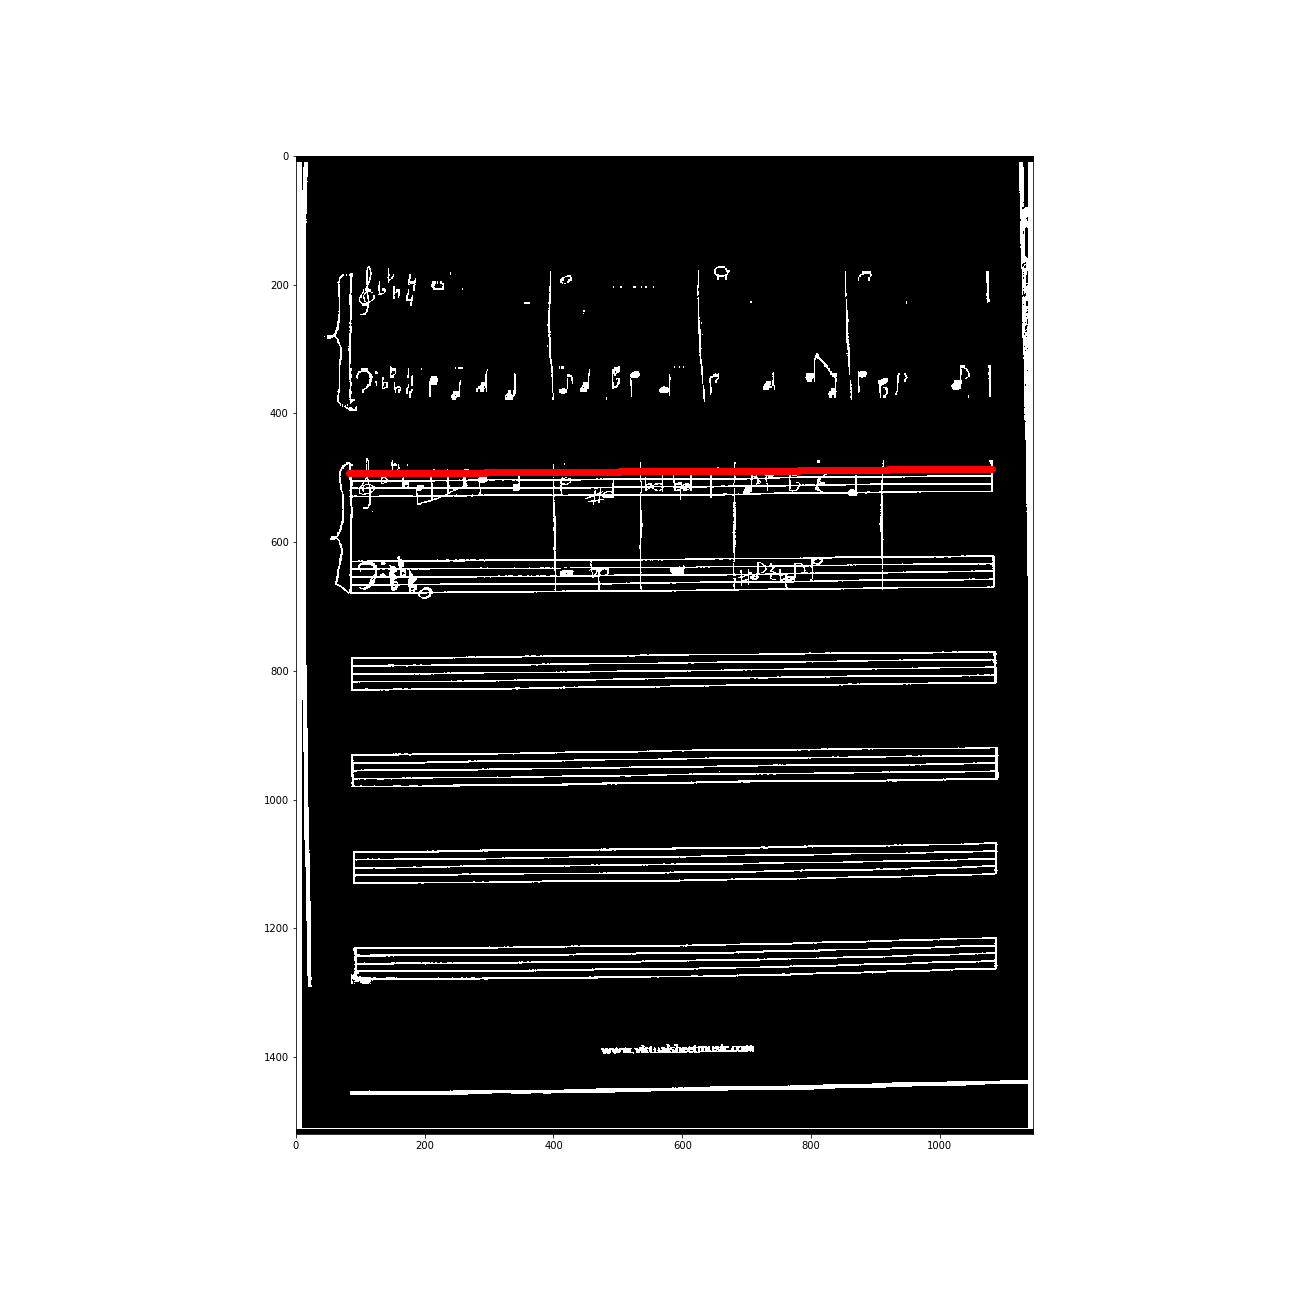
\includegraphics[width=\linewidth]{zdj/BFS12.png}
		\end{subfigure}
		\begin{subfigure}[b]{0.32\linewidth}
			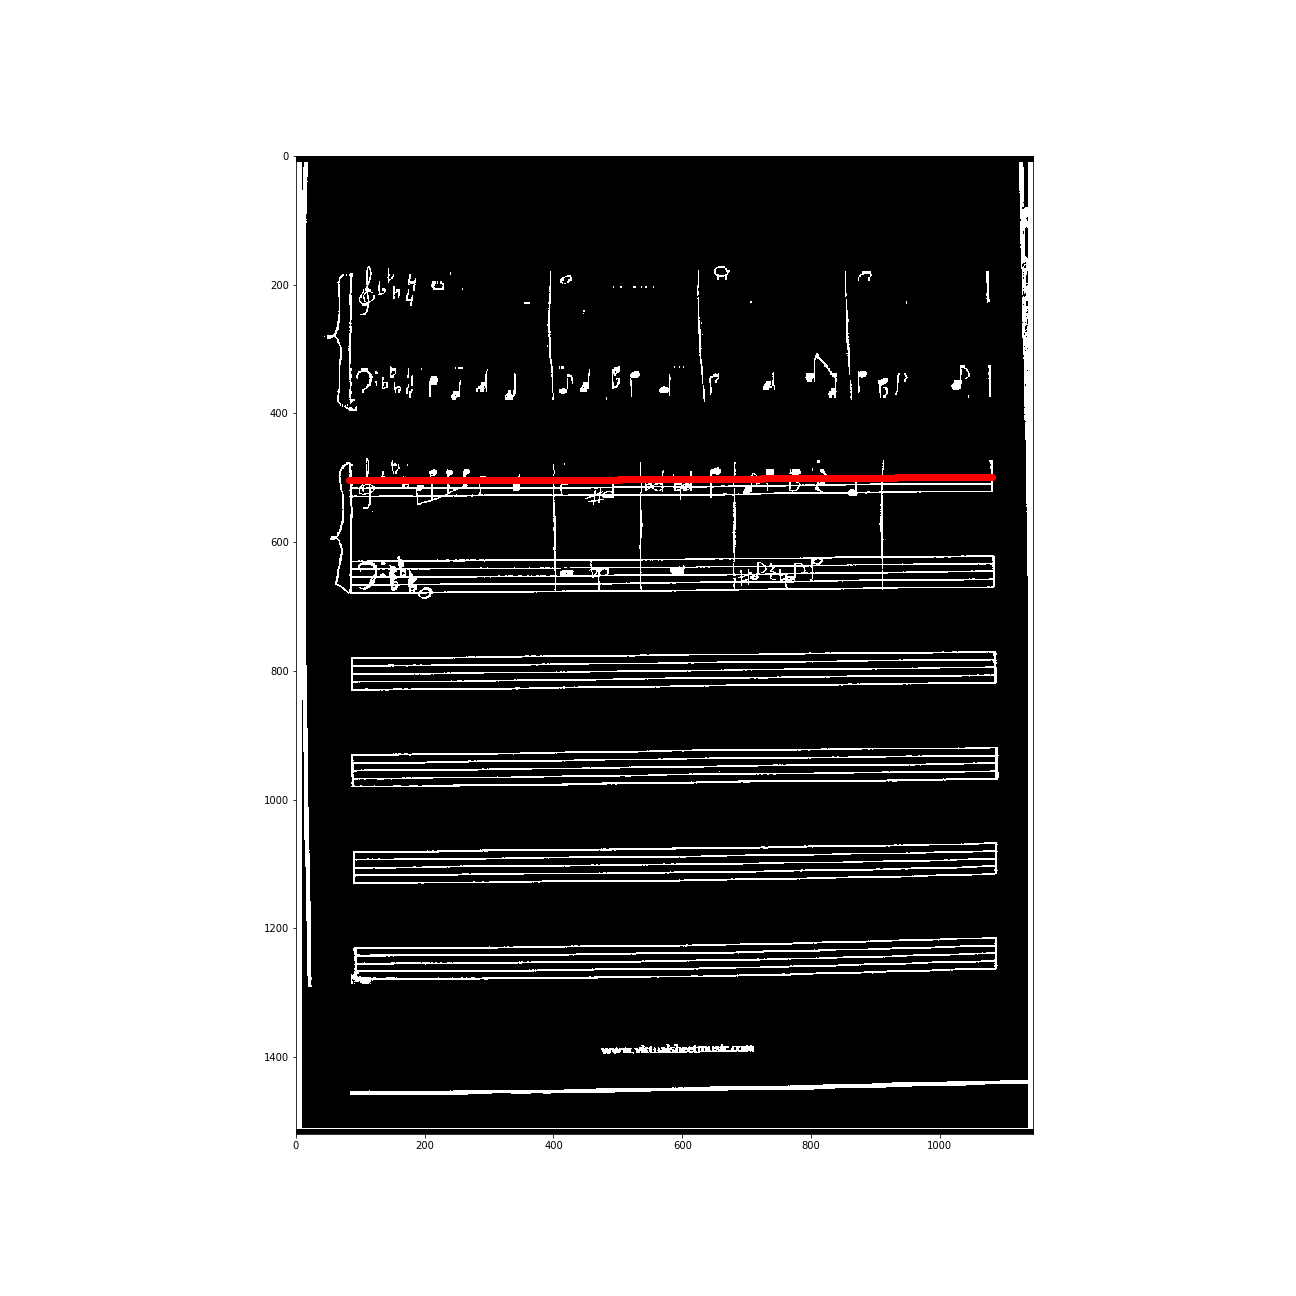
\includegraphics[width=\linewidth]{zdj/BFS13.png}
		\end{subfigure}
		\begin{subfigure}[b]{0.32\linewidth}
			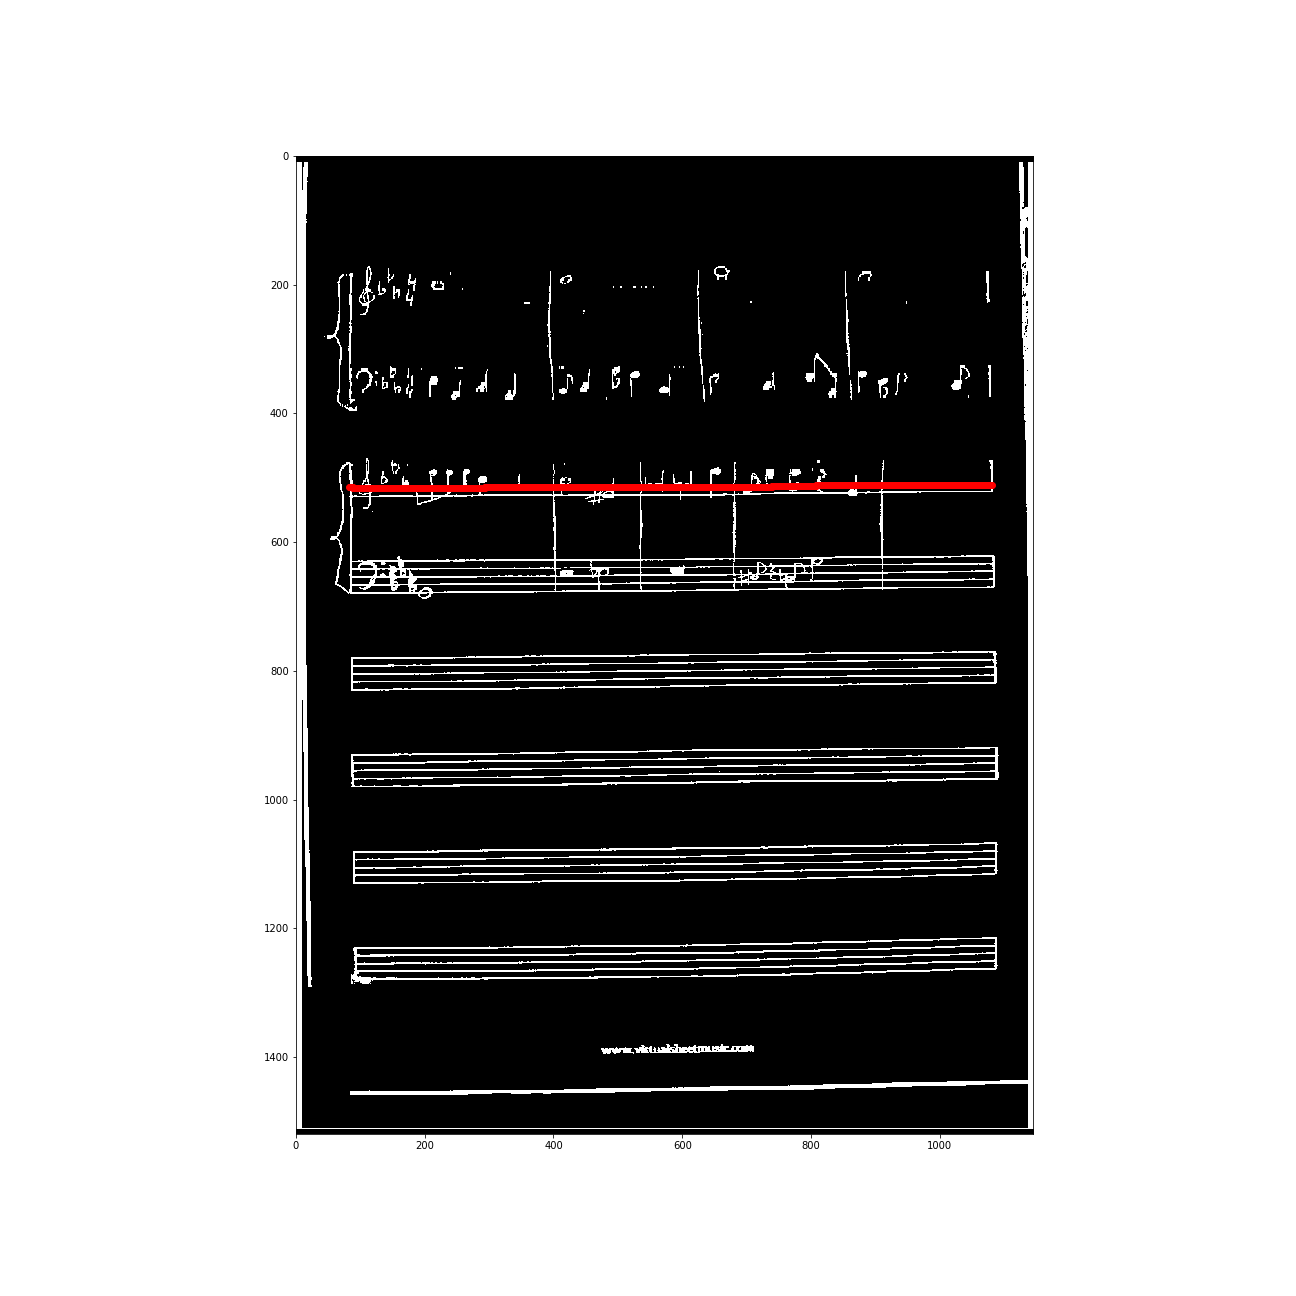
\includegraphics[width=\linewidth]{zdj/BFS14.png}
		\end{subfigure}
		\begin{subfigure}[b]{0.32\linewidth}
			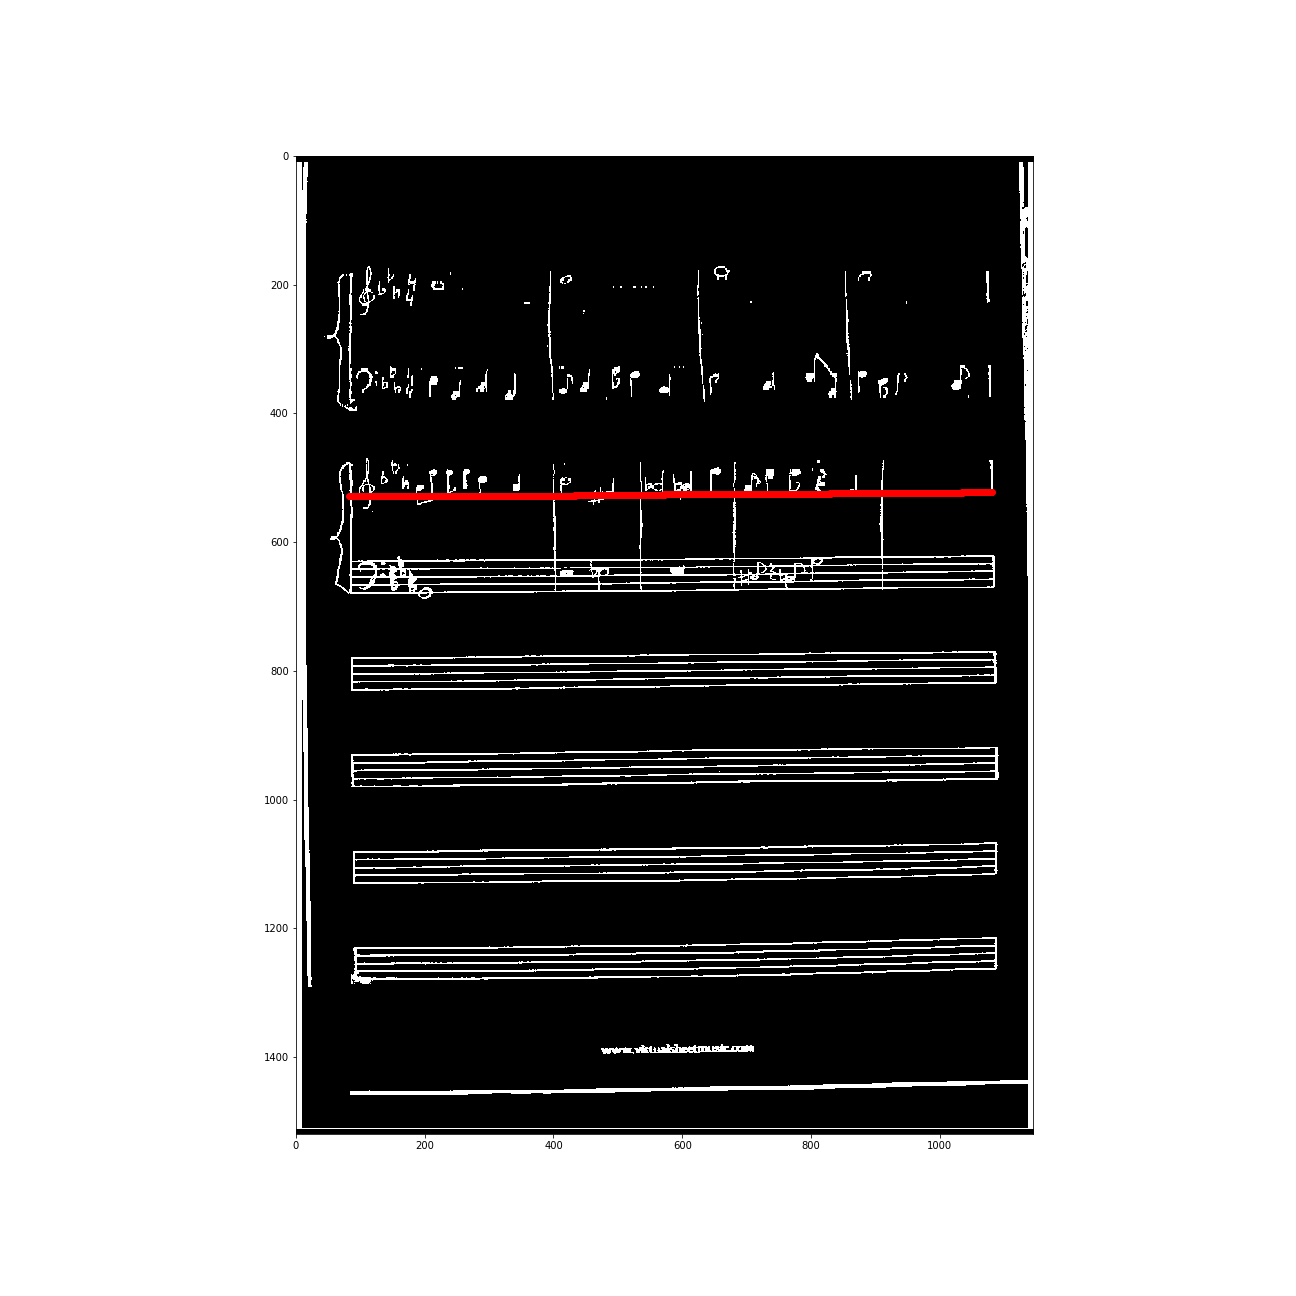
\includegraphics[width=\linewidth]{zdj/BFS15.png}
		\end{subfigure}
		\begin{subfigure}[b]{0.32\linewidth}
			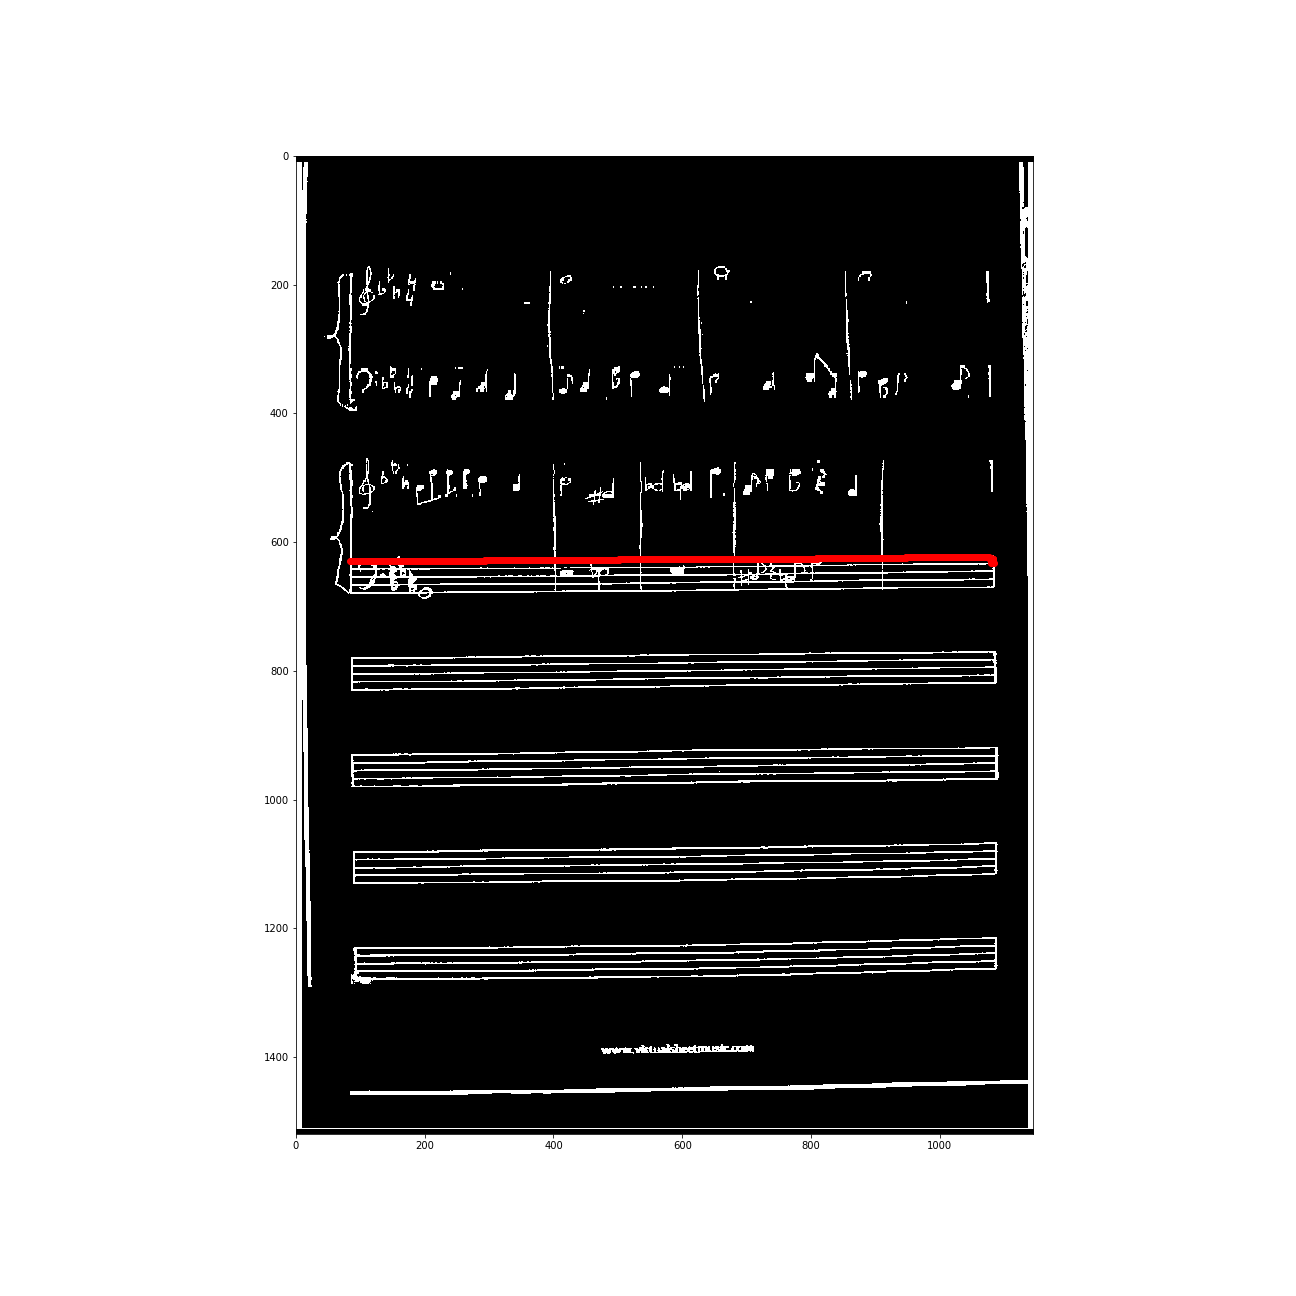
\includegraphics[width=\linewidth]{zdj/BFS16.png}
		\end{subfigure}
		\begin{subfigure}[b]{0.32\linewidth}
			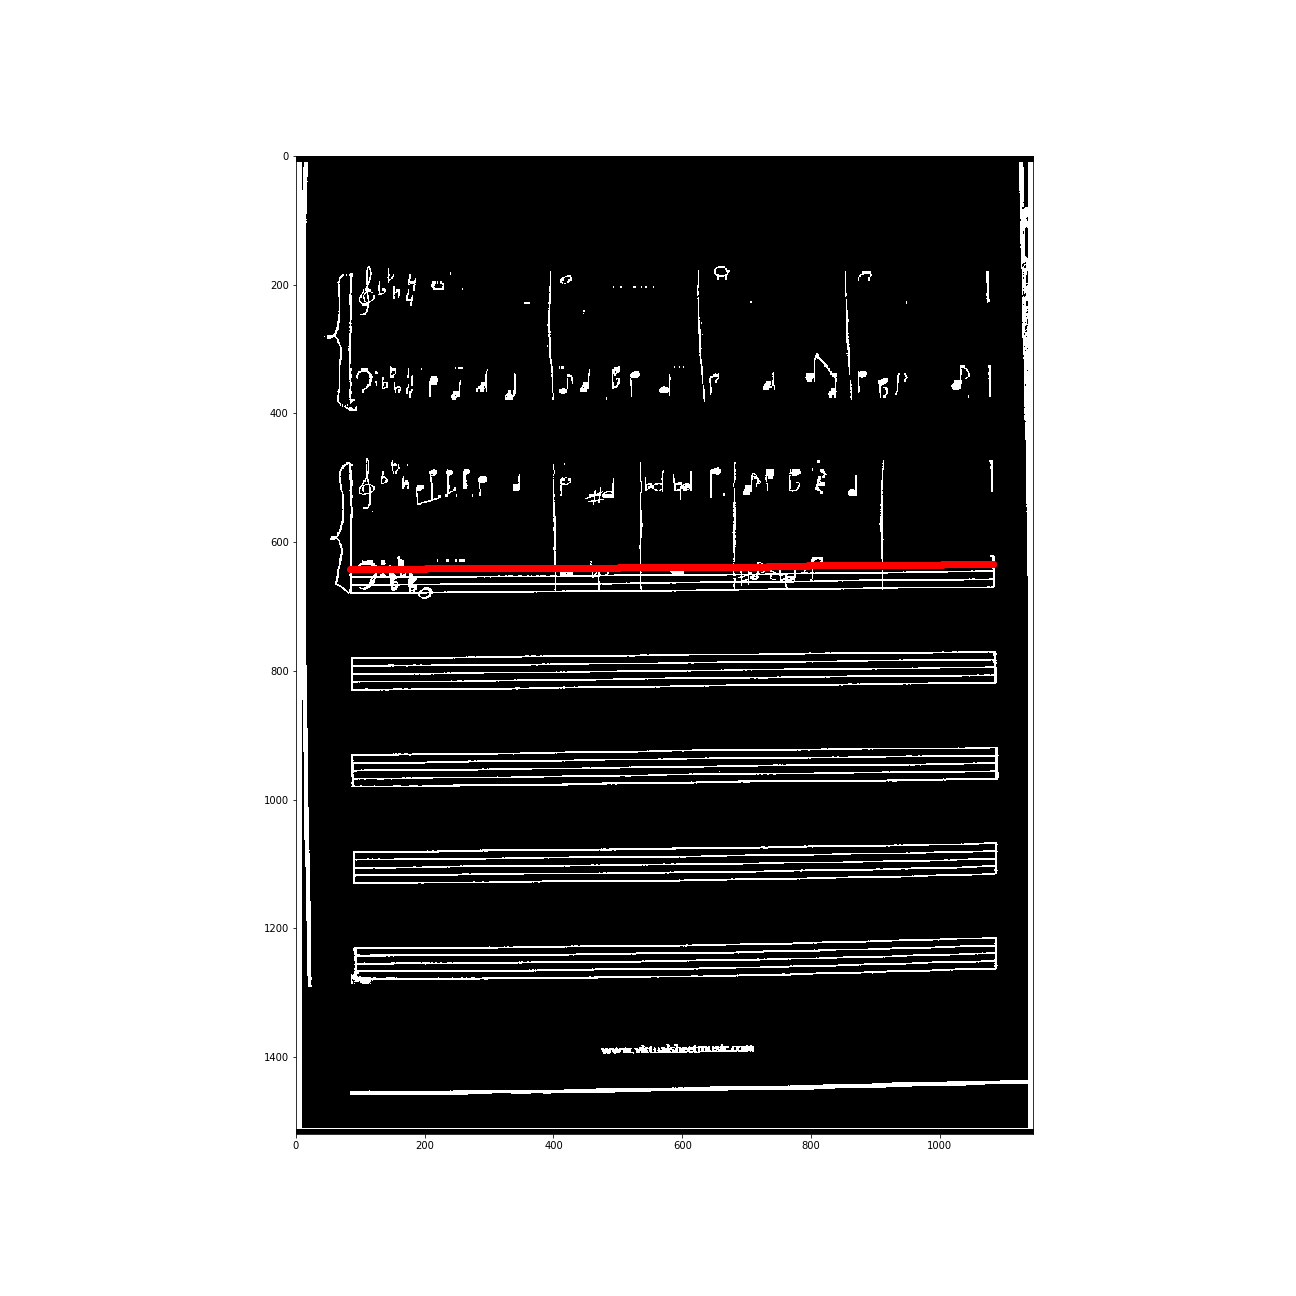
\includegraphics[width=\linewidth]{zdj/BFS17.png}
		\end{subfigure}
		\begin{subfigure}[b]{0.32\linewidth}
			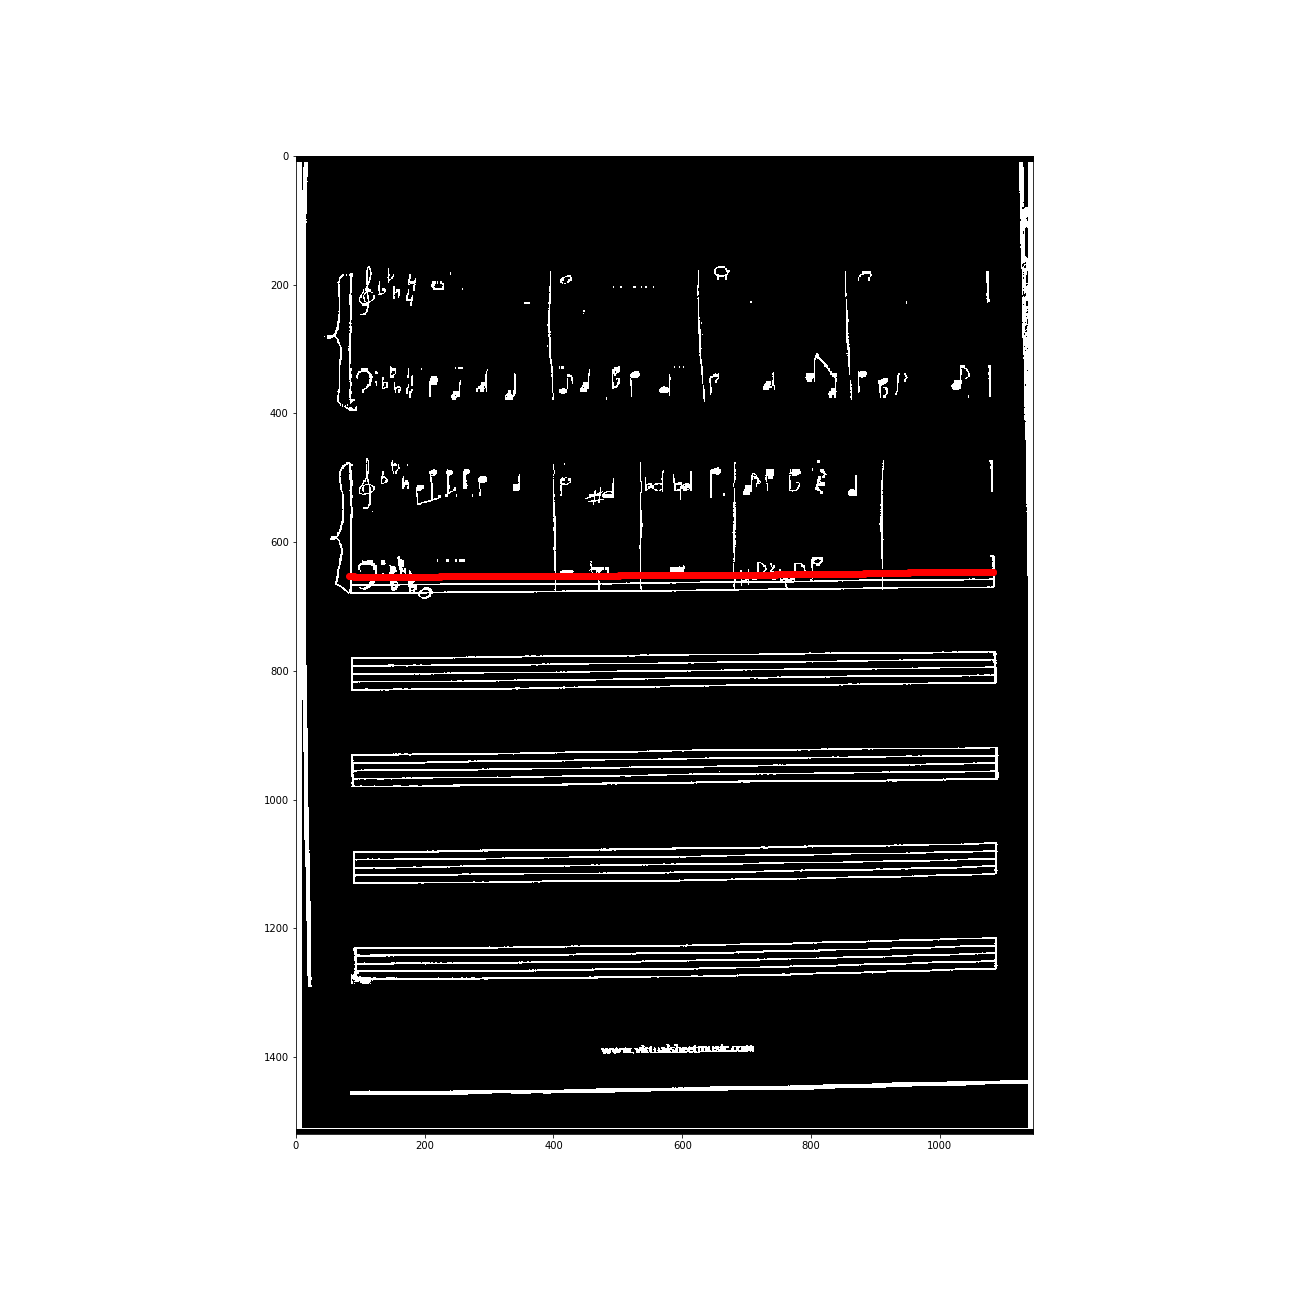
\includegraphics[width=\linewidth]{zdj/BFS18.png}
		\end{subfigure}
		\begin{subfigure}[b]{0.32\linewidth}
			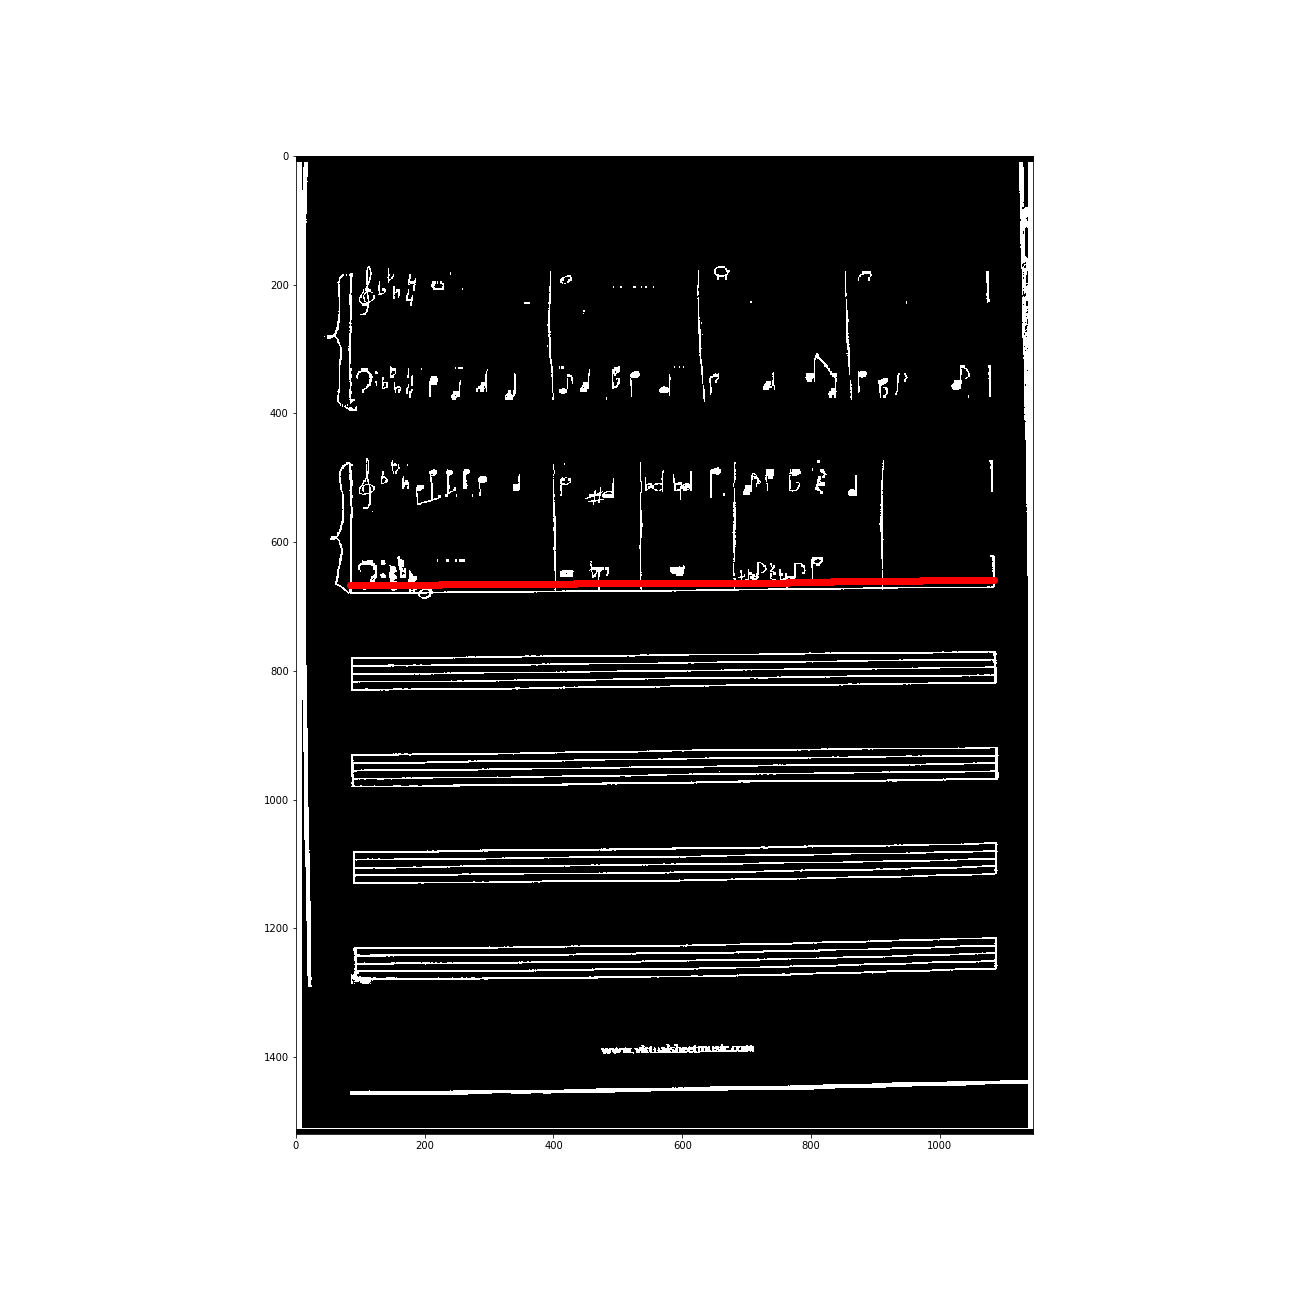
\includegraphics[width=\linewidth]{zdj/BFS19.png}
		\end{subfigure}
		\begin{subfigure}[b]{0.32\linewidth}
			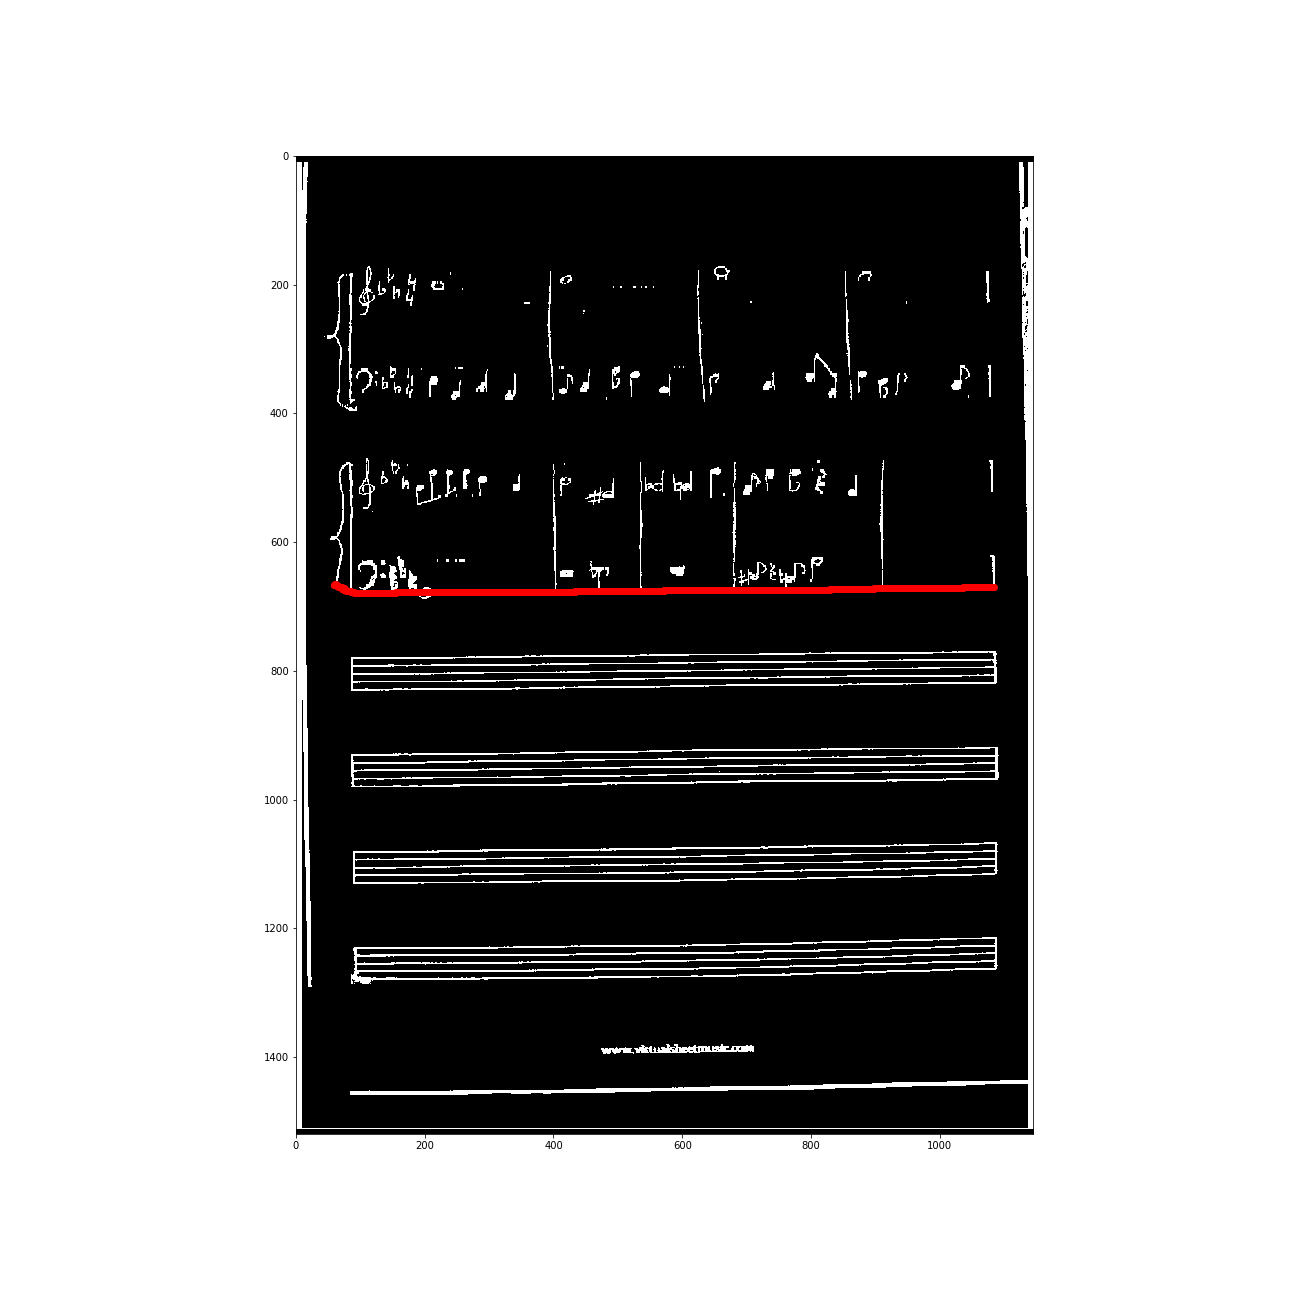
\includegraphics[width=\linewidth]{zdj/BFS20.png}
		\end{subfigure}
		\begin{subfigure}[b]{0.32\linewidth}
			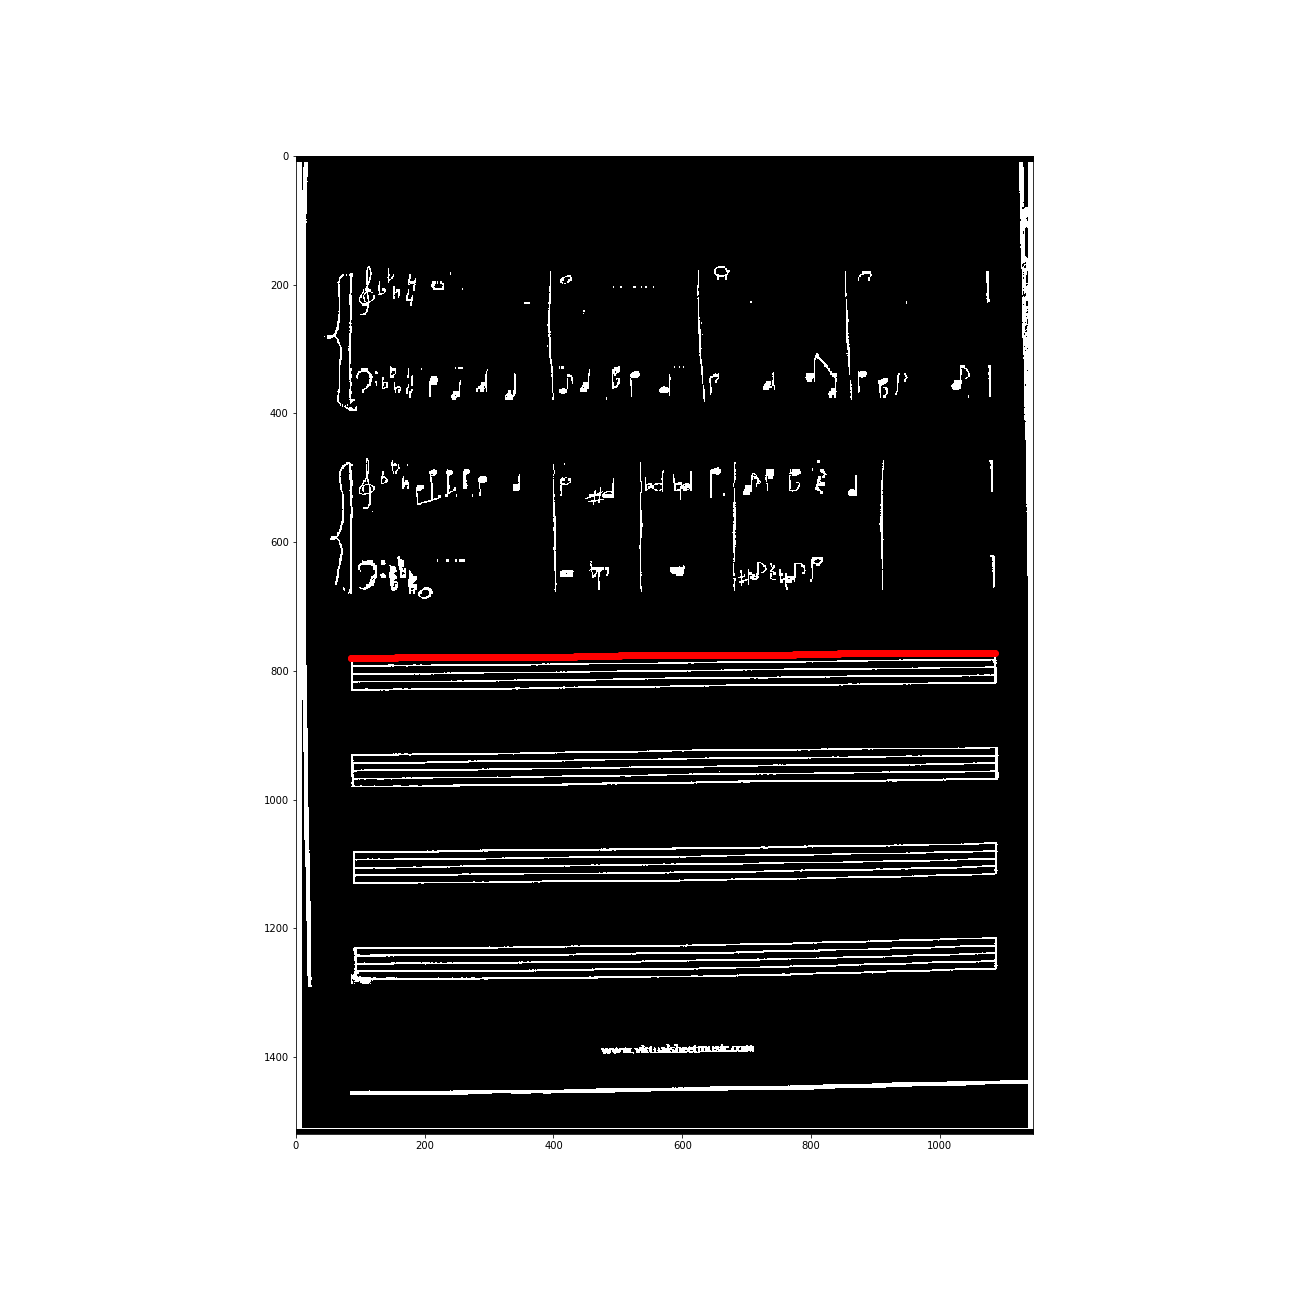
\includegraphics[width=\linewidth]{zdj/BFS21.png}
		\end{subfigure}
		\begin{subfigure}[b]{0.32\linewidth}
			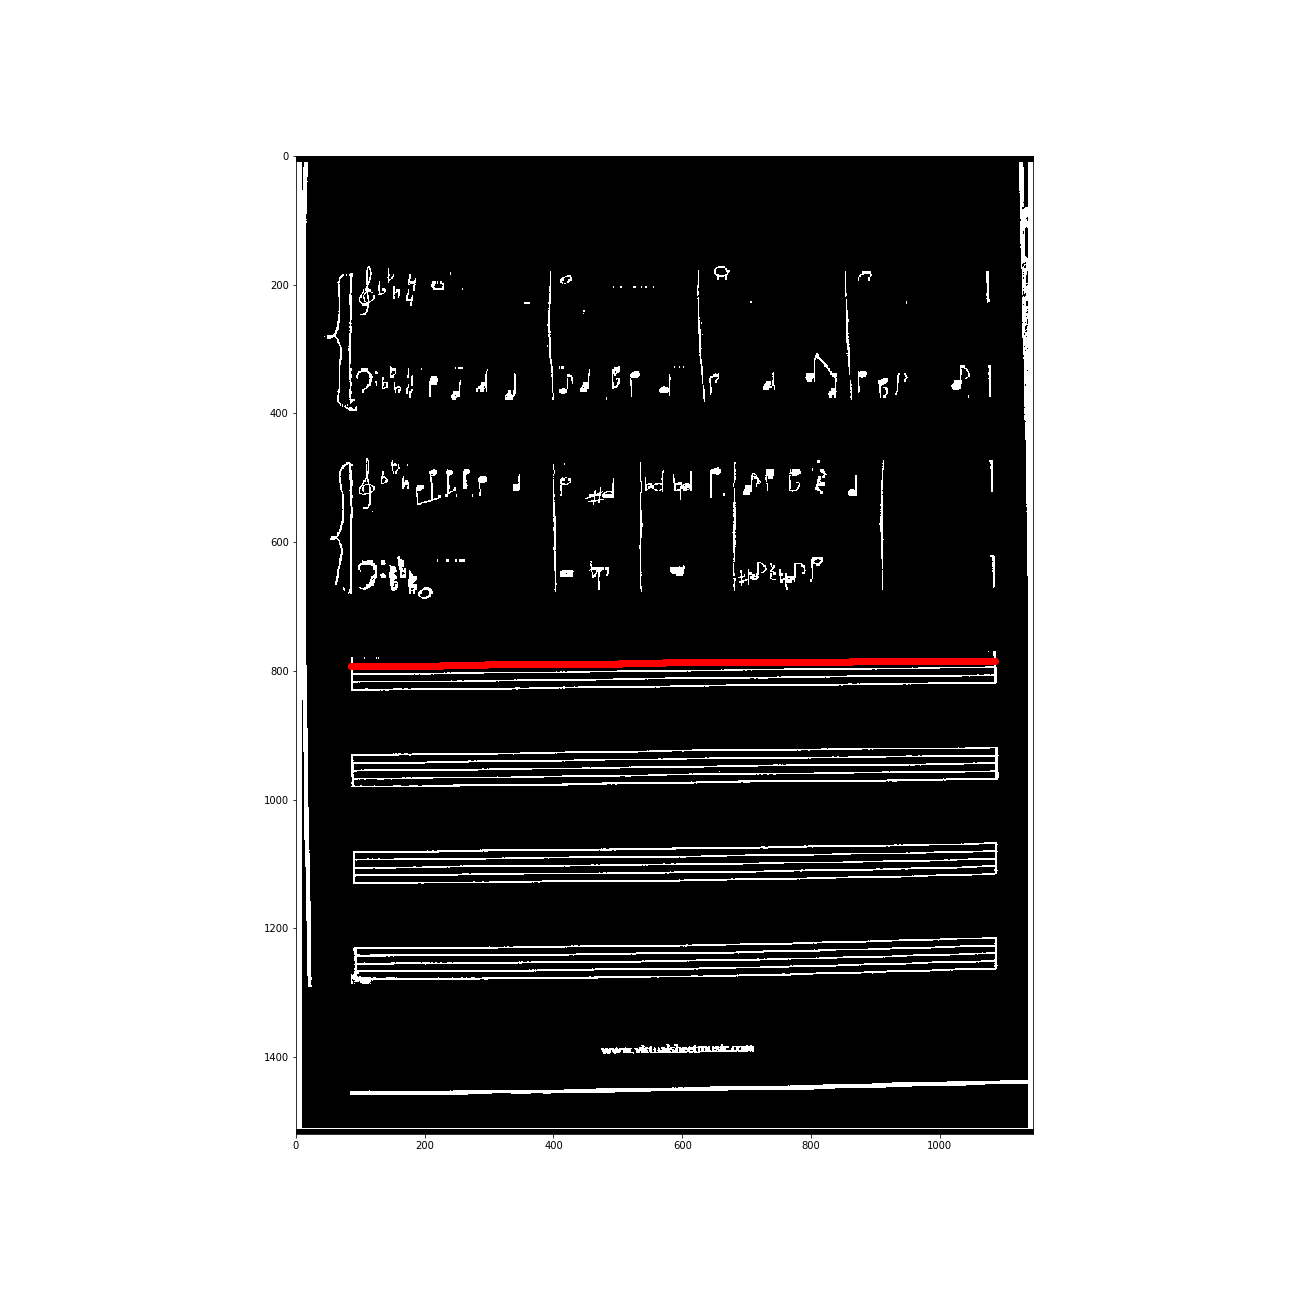
\includegraphics[width=\linewidth]{zdj/BFS22.png}
		\end{subfigure}
		\begin{subfigure}[b]{0.32\linewidth}
			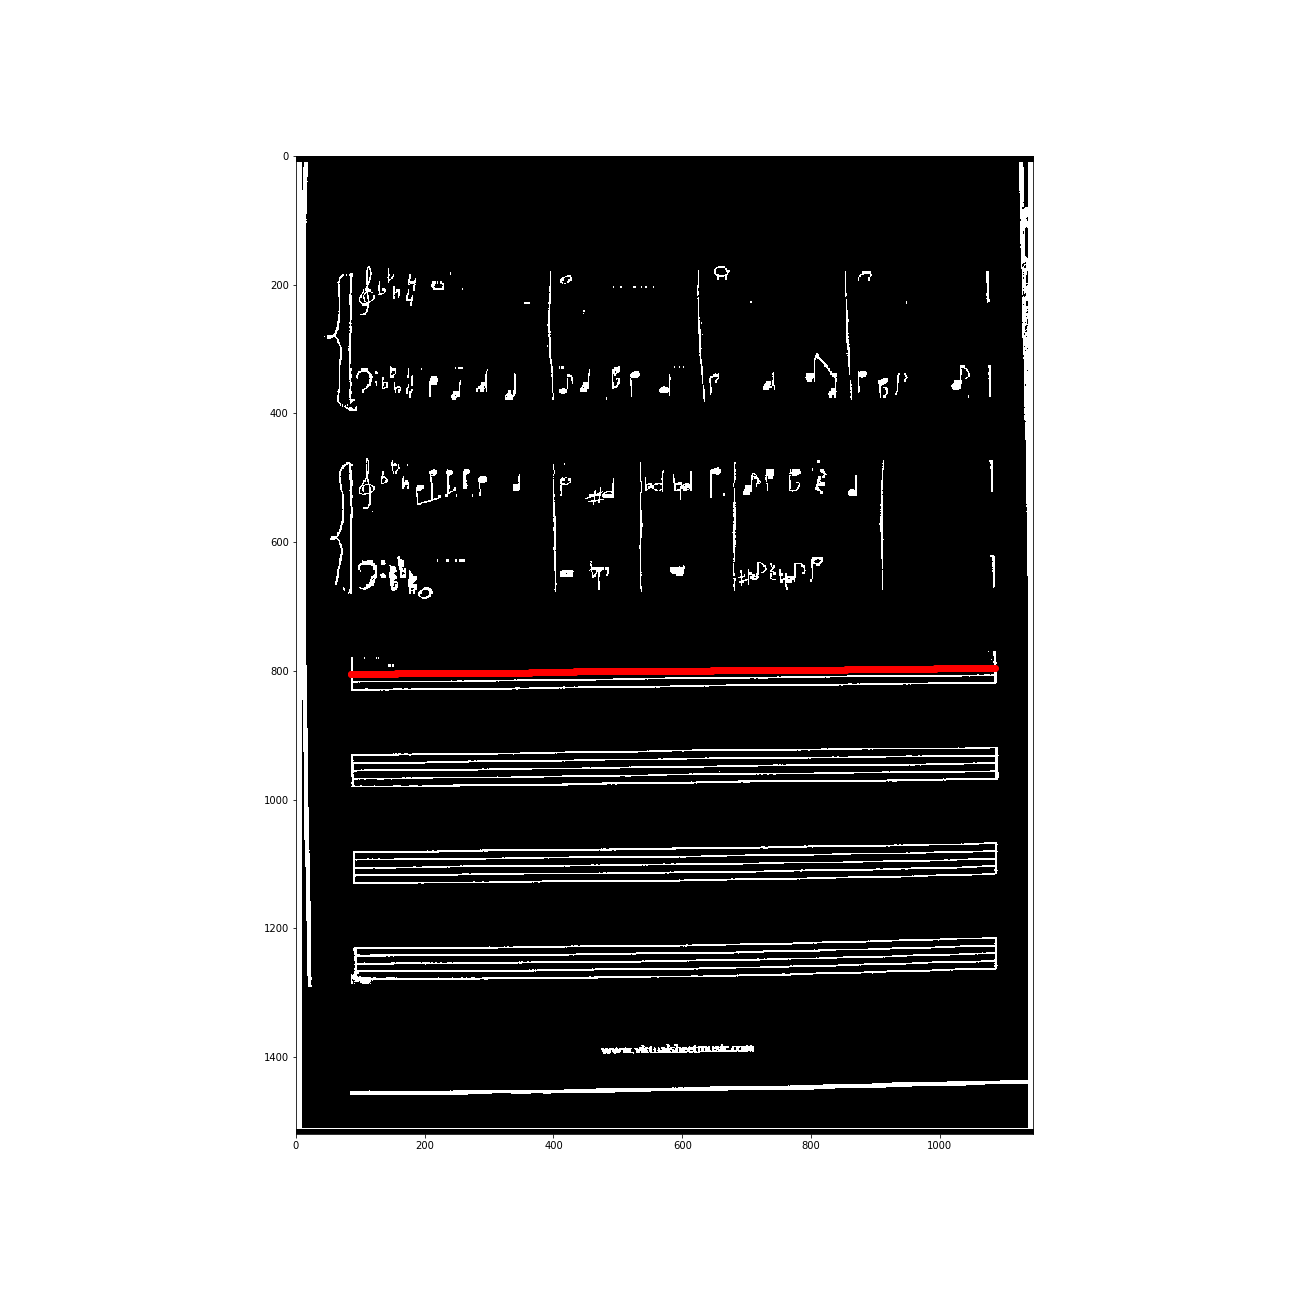
\includegraphics[width=\linewidth]{zdj/BFS23.png}
		\end{subfigure}
		\caption{Proces Detekcji i usuwania linii 2.}
		\label{fig:bfs1}
	\end{figure}

	\begin{figure}[h!]
		\centering
		\begin{subfigure}[b]{0.48\linewidth}
			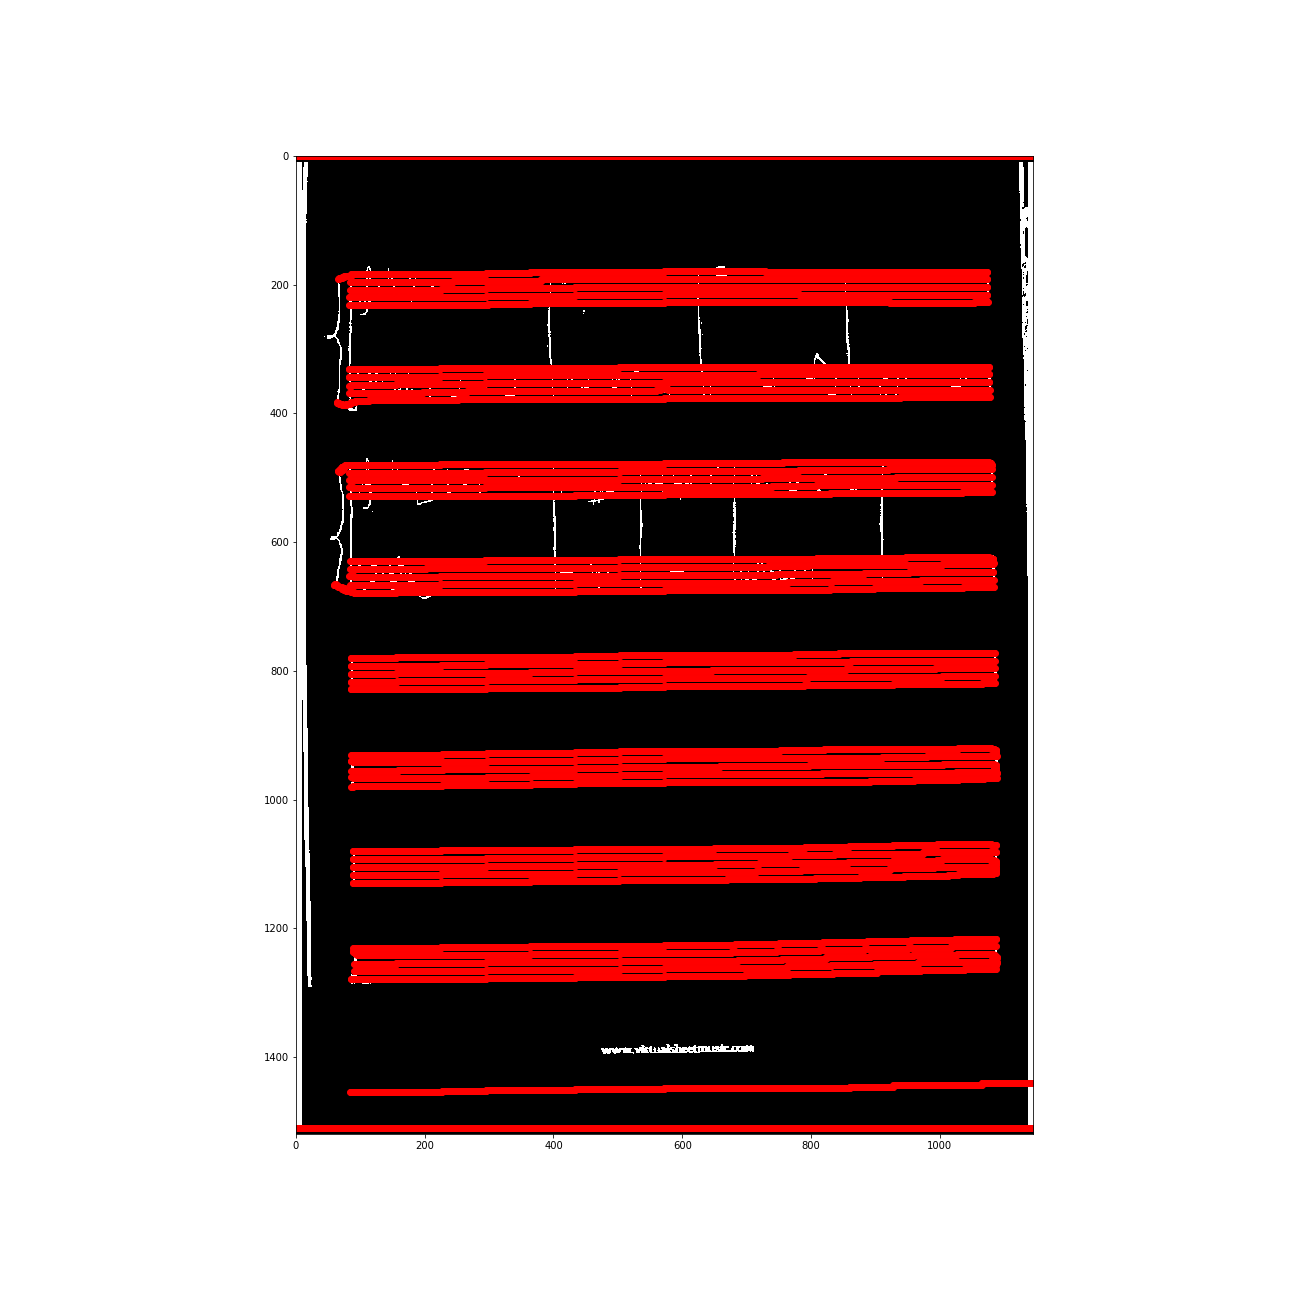
\includegraphics[width=\linewidth]{zdj/BFSFinale0.png}
			\caption{To, co ścięto}
		\end{subfigure}
		\begin{subfigure}[b]{0.48\linewidth}
			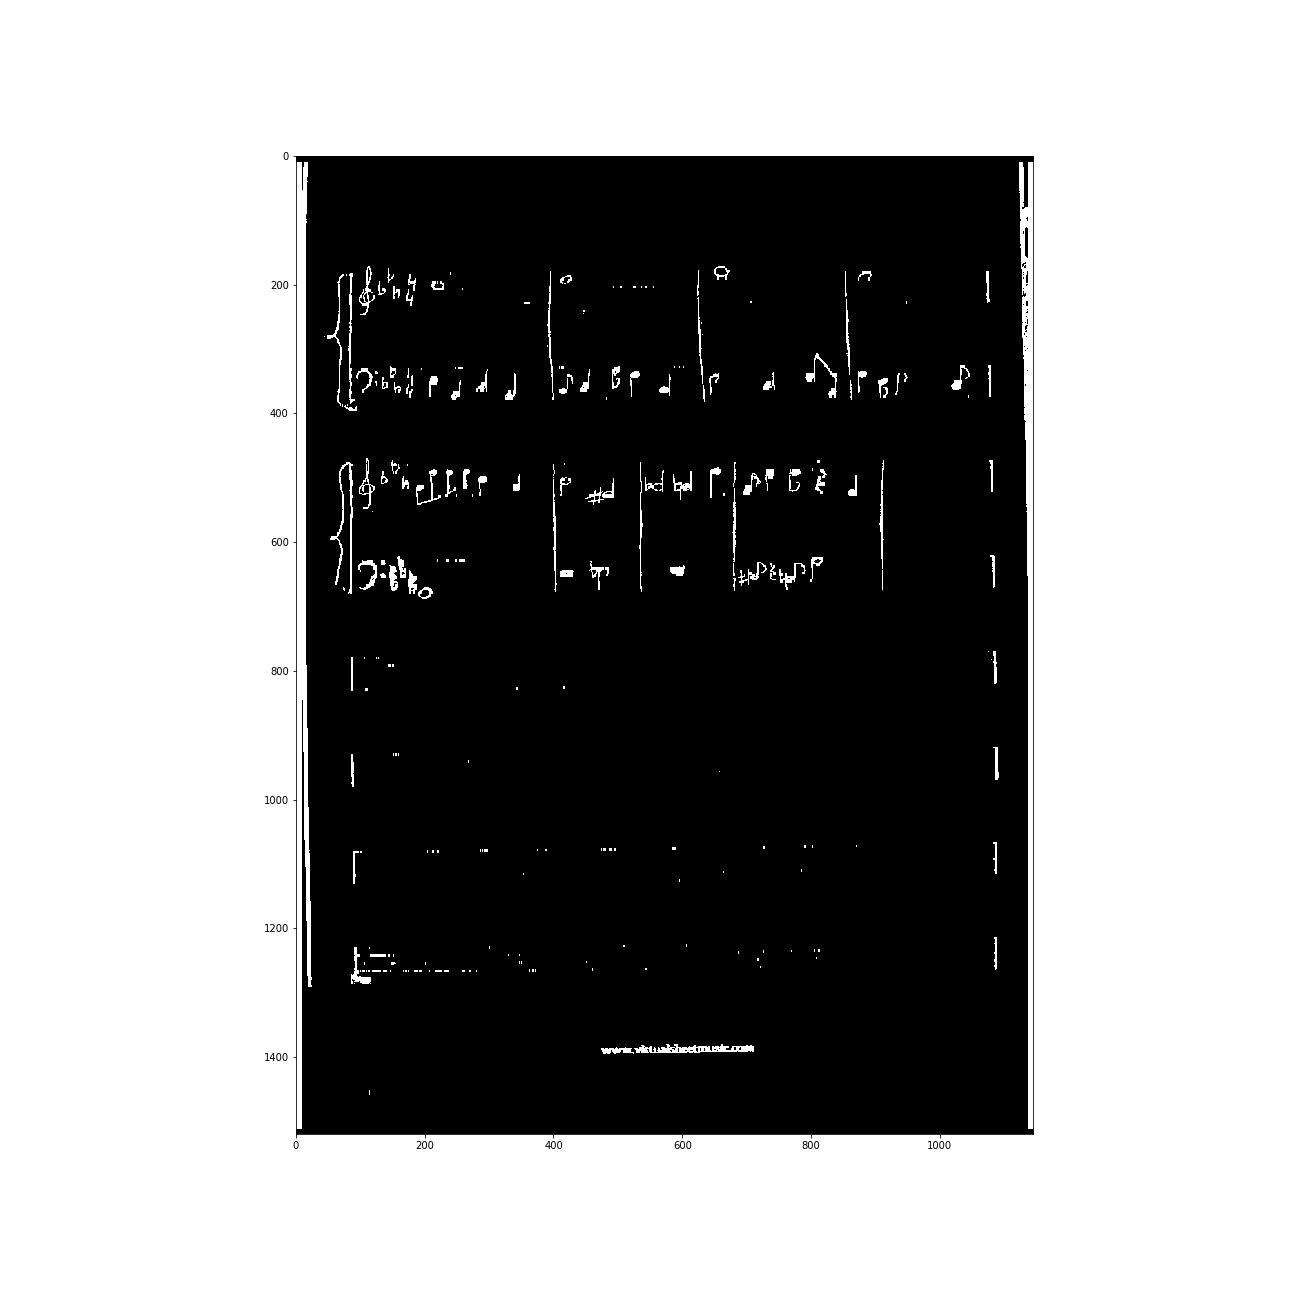
\includegraphics[width=\linewidth]{zdj/BFSFinale1.png}
			\caption{To, co zostało}
		\end{subfigure}
		\caption{Ostateczny efekt BFS-a.}
		\label{fig:bfsfinale}
	\end{figure}
	
	\begin{figure}[h!]
		\centering
		\begin{subfigure}[b]{0.48\linewidth}
			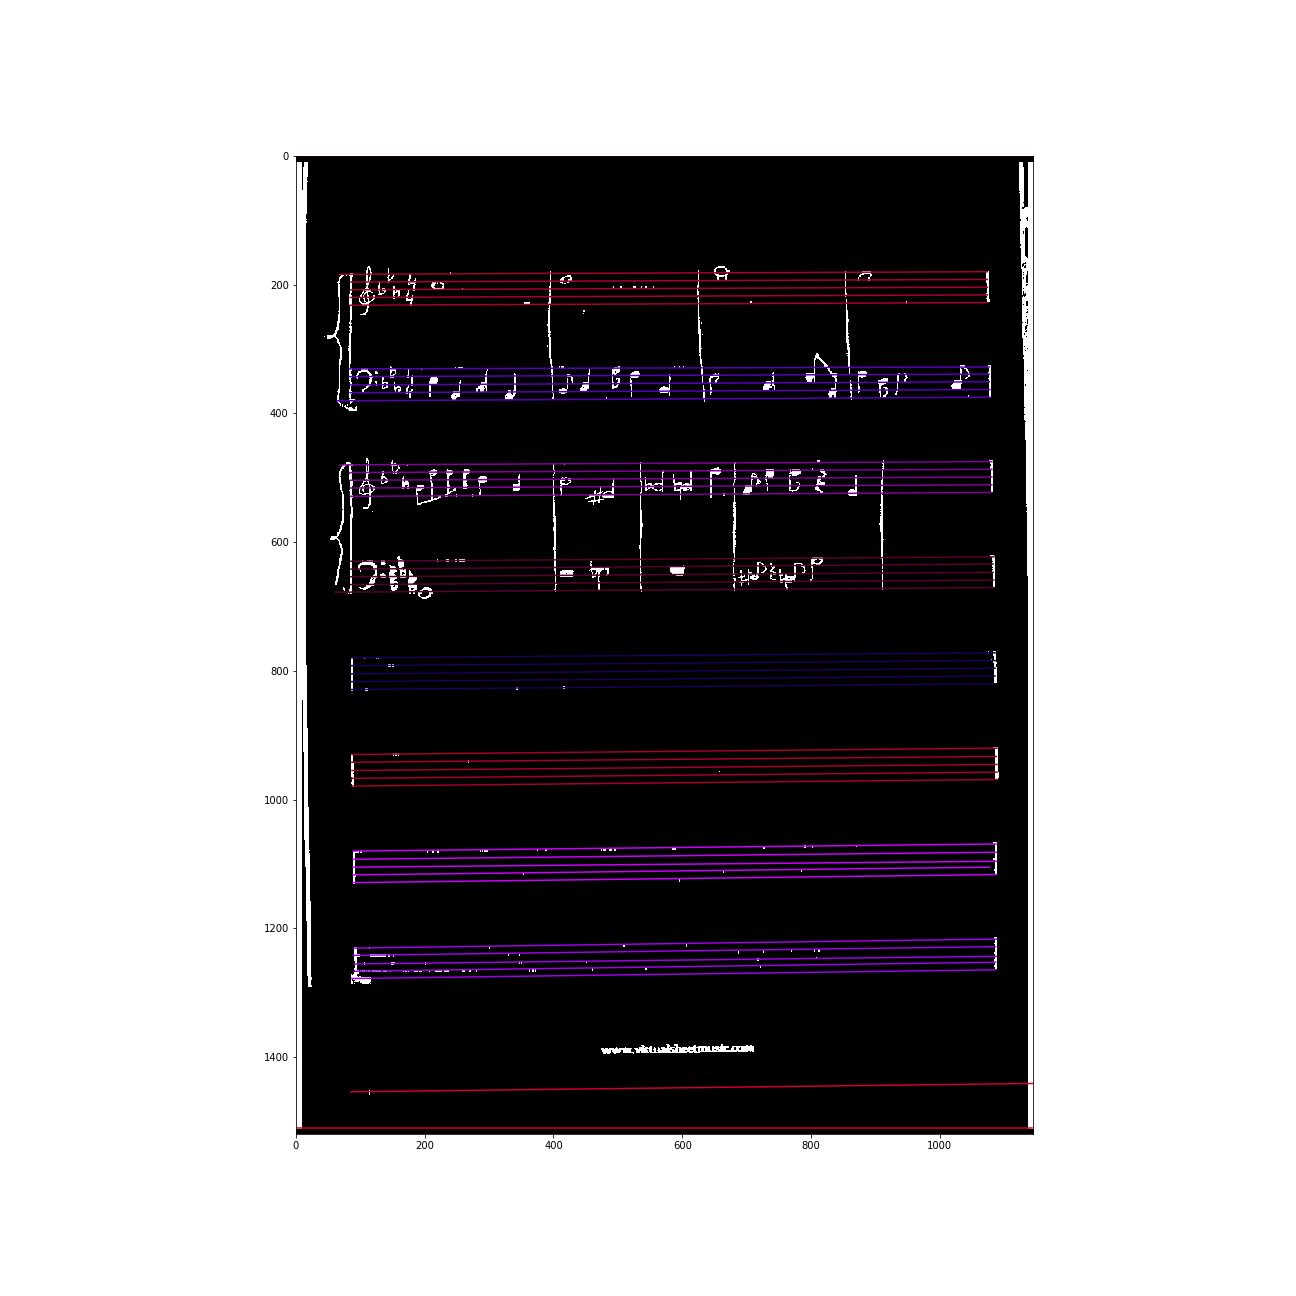
\includegraphics[width=\linewidth]{zdj/5l0.png}
			\caption{Wszystkie linie zgrupowane}
		\end{subfigure}
		\begin{subfigure}[b]{0.48\linewidth}
			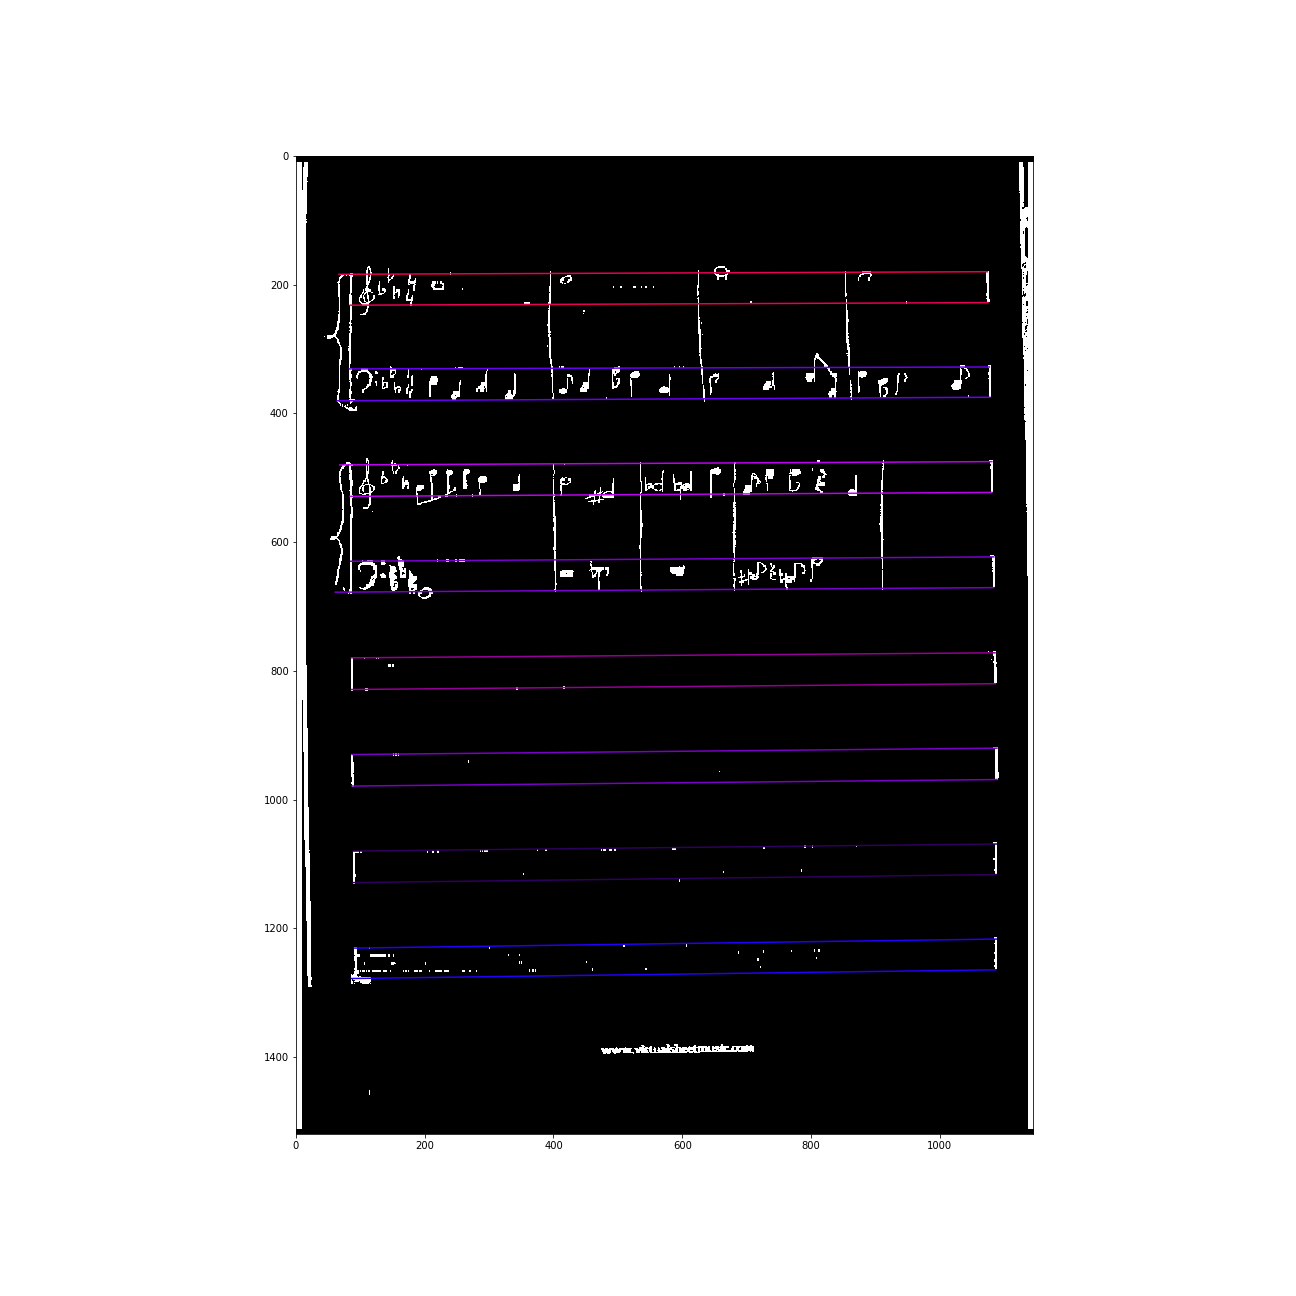
\includegraphics[width=\linewidth]{zdj/5l1.png}
			\caption{Linie po odsiewie}
		\end{subfigure}
		\caption{Poszukiwanie pięciolinii}
		\label{fig:5l}
	\end{figure}
	
	\clearpage
	\section{Detekcja nut}
		Kolejnym krokiem jest detekcja nut na przetworzonym obrazku.
		\begin{enumerate}
			\item Najpierw liczę rozmiary pięciolinii. Wysokość, początek i koniec są wyliczane na podstawie linii otrzymanych w poprzedniej części - biorę medianę z tych wymiarów.
			\item Kolejnym krokiem jest oczyszczenie pięciolinii. Jeśli ich długość lub wysokość odbiega za bardzo od mediany to zmieniam ich rozmiary.
			\item Następnie klasyfikuję klucze będące na początku pięciolinii. Robię to patrząc na ilość bieli na początku - więcej to klucz wiolinowy, mniej - klucz basowy.
			\item Czwartym krokiem jest detekcja główek nut:
				\begin{enumerate}
					\item Najpierw zmieniam rozmiar wzorców zależnie od mediany wysokości pięciolinii.
					\item Następnie znajduję dopasowania wzorca (używam znormalizowanej różnicy kwadratów). Do zwróconych wartości stosuję progowanie. To co poniżej progu jest nutą.
					\item Jeśli znalazłem w małym obszarze wiele dopasowań to biorę to które ma najmniejszą wartość.
					\item Powtarzam to dla trzech wzorców - główki wypełnionej, półnuty oraz całej nuty. Jeśli dopasowania się nakładają to zostawiam tylko pierwsze dopasowanie.
					\item Wielkość wzorca określa prostokąt ograniczający nutę - środek prostokąta uznaję za środek nuty.
				\end{enumerate}
			\item Teraz odfiltrowuję znalezione główki nut - jeśli są za bardzo na lewo lub na prawo od pięciolinii lub za daleko od środka najbliższej pięciolinii to je usuwam.
			\item Określam wysokość nuty - najpierw znajduję pięciolinię której środek jest najbliżej nuty. Dla tej pięciolinii obliczam średnią współrzędną y dolnej i górnej linii oraz wysokość. Na podstawie odległości środka nuty od dolnej linii określam gdzie na pięciolinii nuta leży (to jest która linia lub przerwa). Znając położenie nuty oraz klucz danej pięciolinii mogę określić wysokość nuty.
			\item Kolejnym etapem jest określenie długości nuty
				\begin{enumerate}
					\item Najpierw określam czy główka nuty jest wypełniona czy nie. Robię to patrząc na średni kolor środka nuty na oryginalnym obrazku.
					\item Kolejnym krokiem jest znalezienie ogonka nuty. W tym celu patrzę na projekcję pionową poniżej i powyżej nuty i określam czy jest tam odpowiednio wysokie maksimum. Jeśli jest to próbuję znaleźć koniec laseczki przechodząc po białych pikselach, pionowo, tam gdzie znalazłem maksimum. Czasem część laseczki jest usunięta - algorytm może ominąć 3 czarne piksele.
					\item Jeśli nuta była pusta w środku i znalazłem ogonek nuty to jest to półnuta, jeśli nie to cała nuta. Jeśli główka była wypełniona i nie znalazłem ogonka to taką nutę usuwam.
					\item Następnie określam czy dana nuta to ósemka. Najpierw używam projekcji "po przekątnej" - średnia koloru na prawo od nuty i odpowiednio na dół lub do góry, pod kątem $45\deg$. Jeśli jest tam odpowiednio wysokie maksimum to jest to flaga ósemki. Jeśli tak nie jest to sprawdzam czy na lewo lub na prawo od końca ogonka nuty jest odpowiednio dużo białego - to jest daszek ósemki.
				\end{enumerate}
			\item Przedostatni krok to znalezienie krzyżyków. Najpierw sprawdzam dla każdej nuty pewien obszar przed nią: sprawdzam maksimum w projekcji wertykalnej i horyzontalnej - muszą być odpowiednio duże. Średni kolor też musi być odpowiednio duży. Jeśli te warunki są spełnione to sprawdzam czy obszar nie nakłada się na inną nutę - jeśli tak to odrzucam. Jeśli nie odrzucę obszaru to znajduje się w nim krzyżyk.
			\item Na końcu wyświetlam na obrazku prostokąty ograniczające nuty. Kolory oznaczają: niebieski - cała nuta, cyan - półnuta, zielony - ćwierćnuta, magenta - ósemka. Krzyżyki są zaznaczone na żółto, klucz wiolinowy na zielono, basowy na brązowo. Nad nutami wypisuję wysokość nuty.
		\end{enumerate}
	
		\begin{figure}[h!]
			\centering
			\begin{subfigure}[b]{0.32\linewidth}
				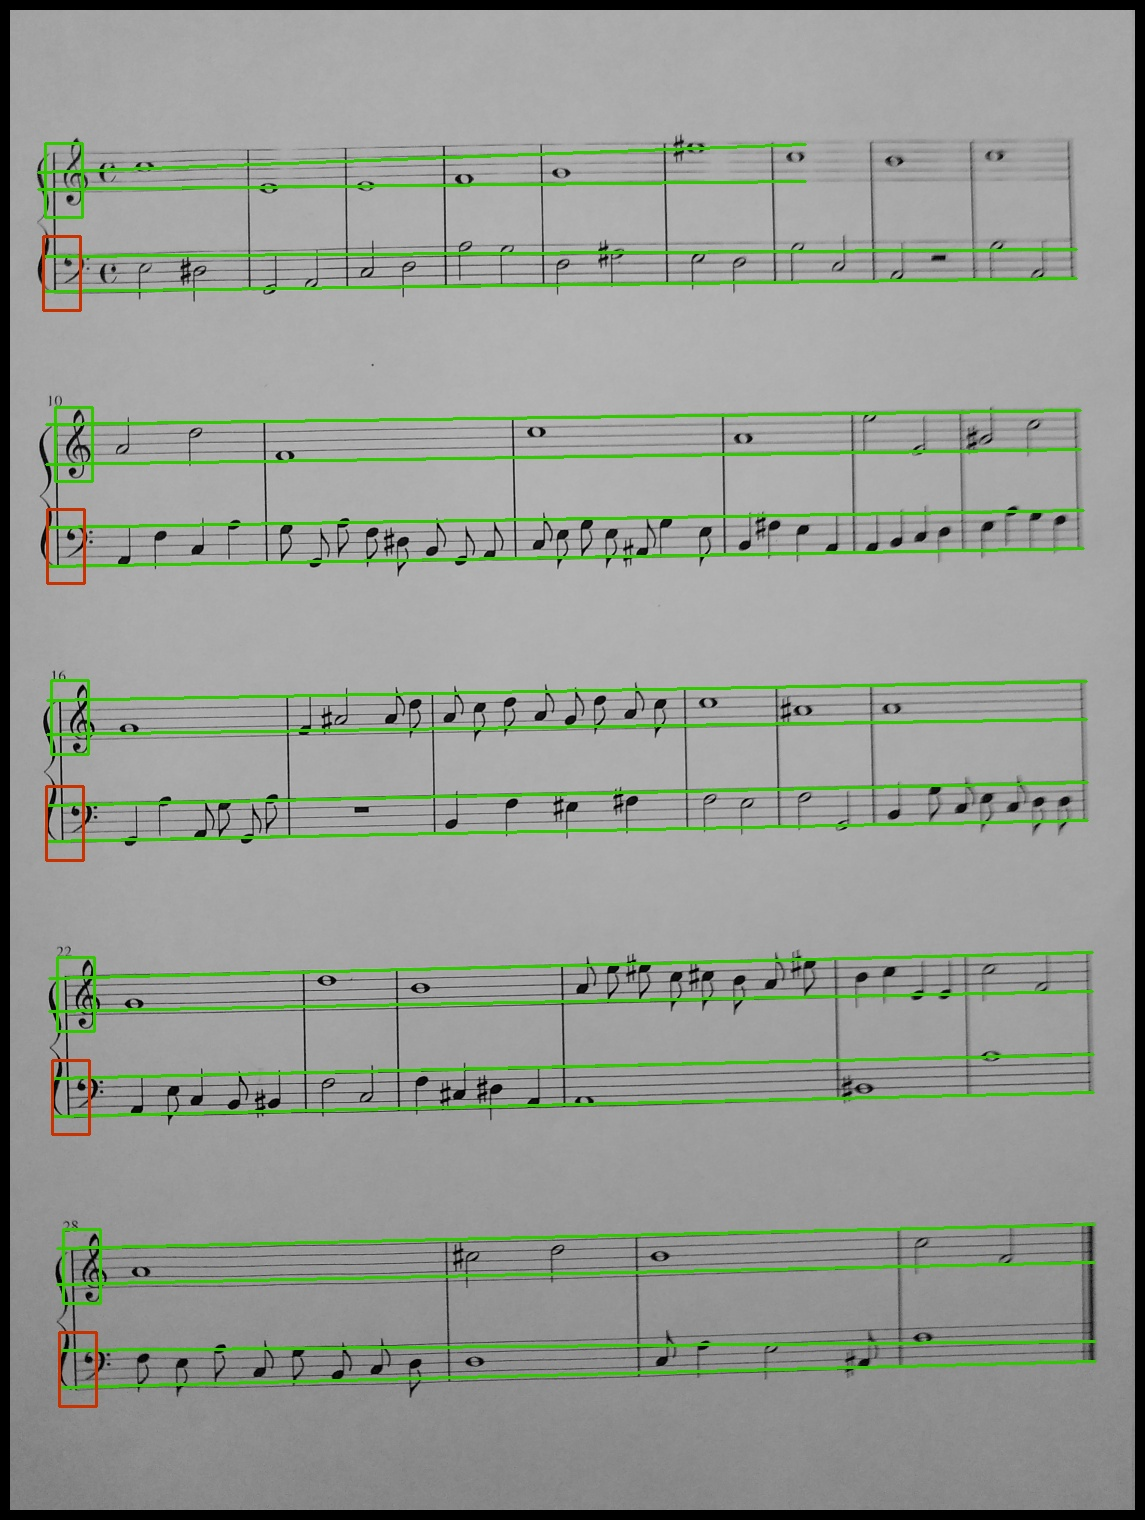
\includegraphics[width=\linewidth]{zdj/step_1.jpg}
				\caption{Klucze i pięciolinie}
			\end{subfigure}
			\begin{subfigure}[b]{0.32\linewidth}
				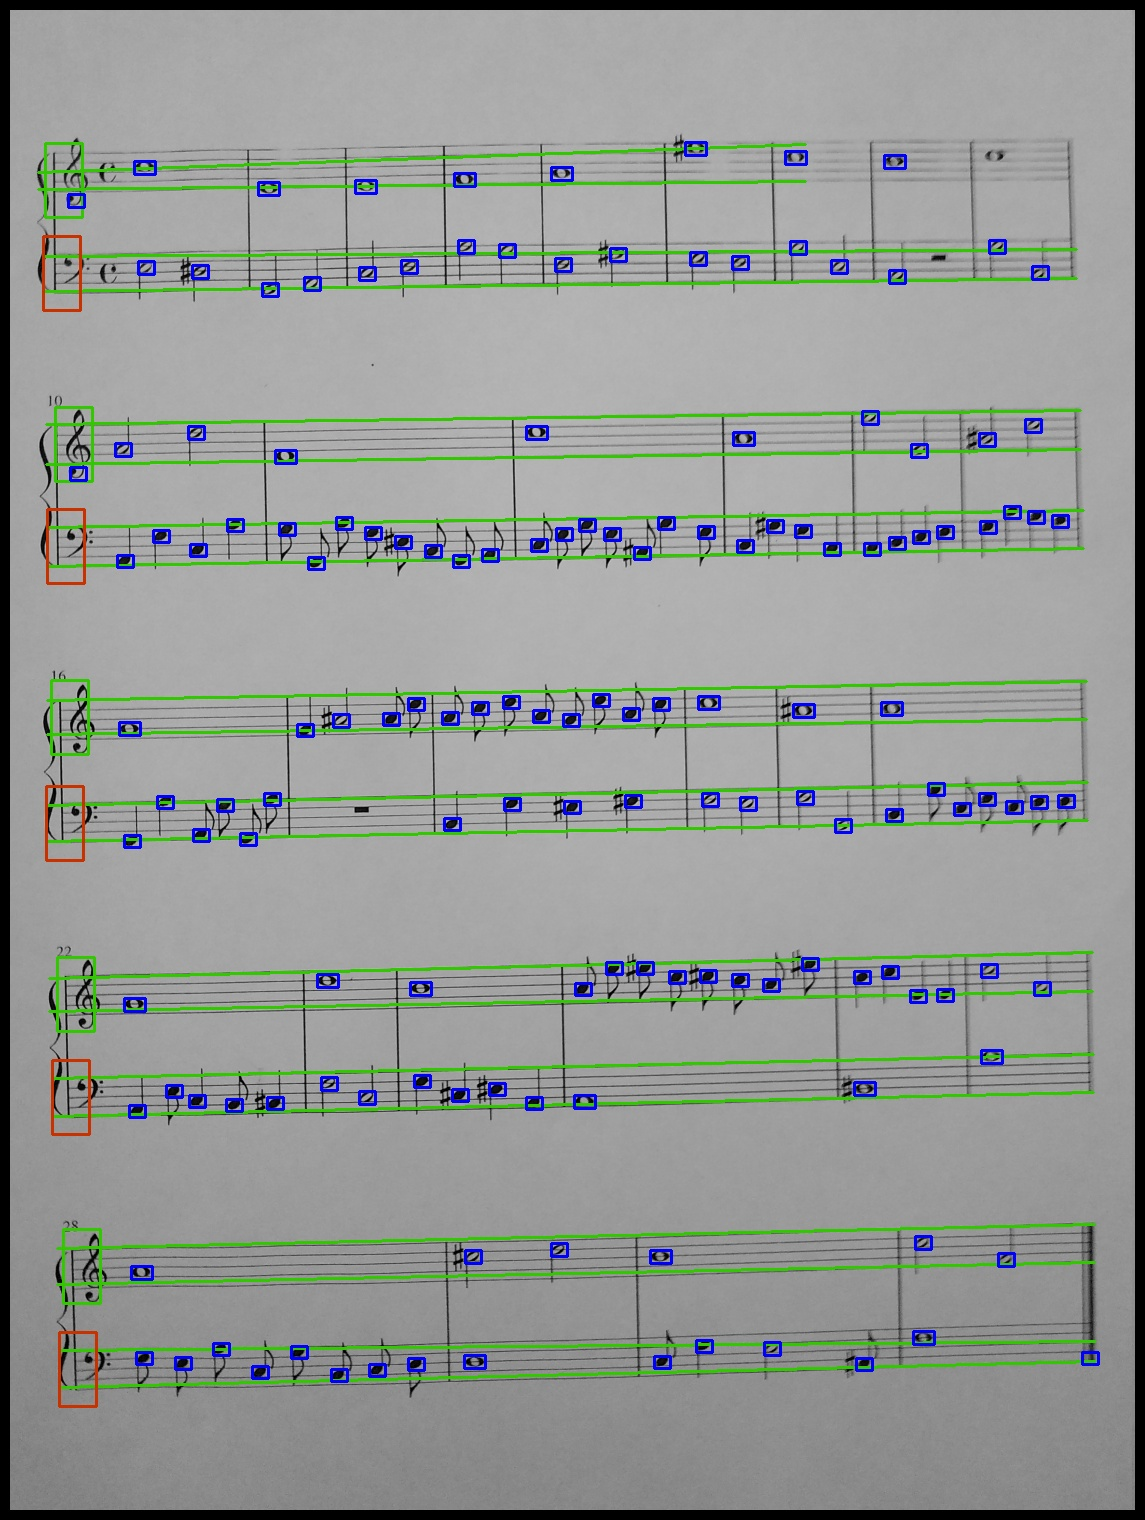
\includegraphics[width=\linewidth]{zdj/step_2.jpg}
				\caption{Wykryte główki nut}
			\end{subfigure}
			\begin{subfigure}[b]{0.32\linewidth}
				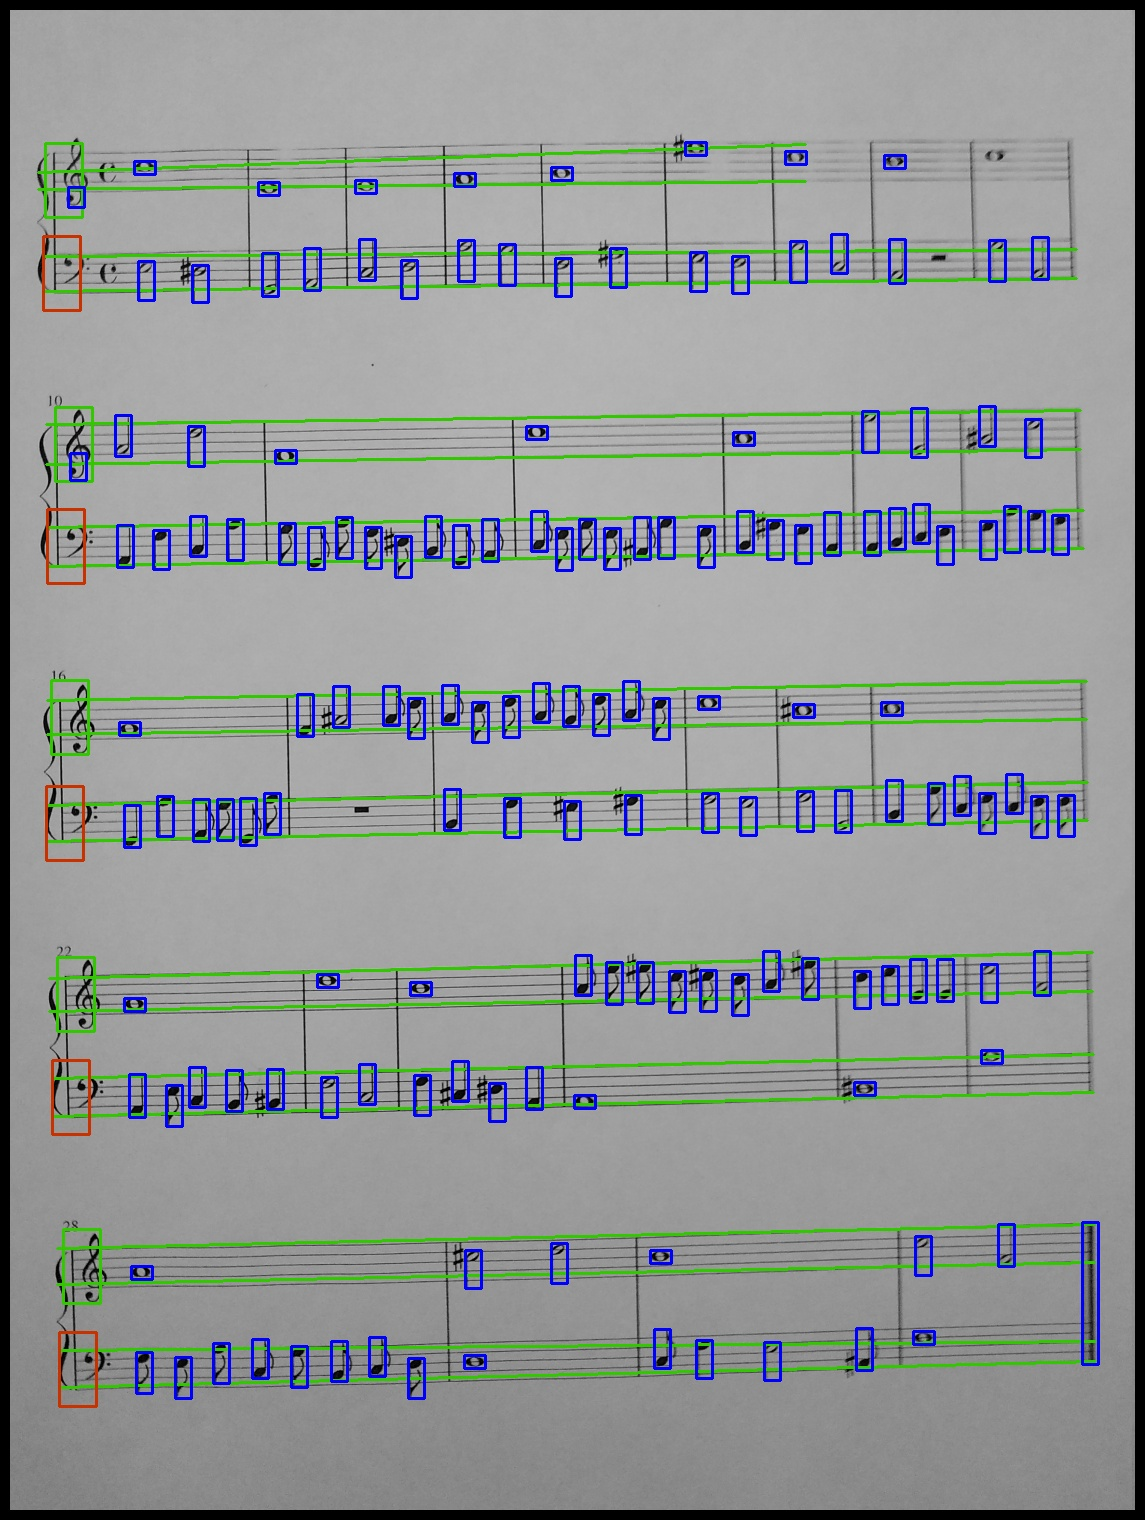
\includegraphics[width=\linewidth]{zdj/step_3.jpg}
				\caption{Nuty z ogonkami}
			\end{subfigure}
			\begin{subfigure}[b]{0.32\linewidth}
				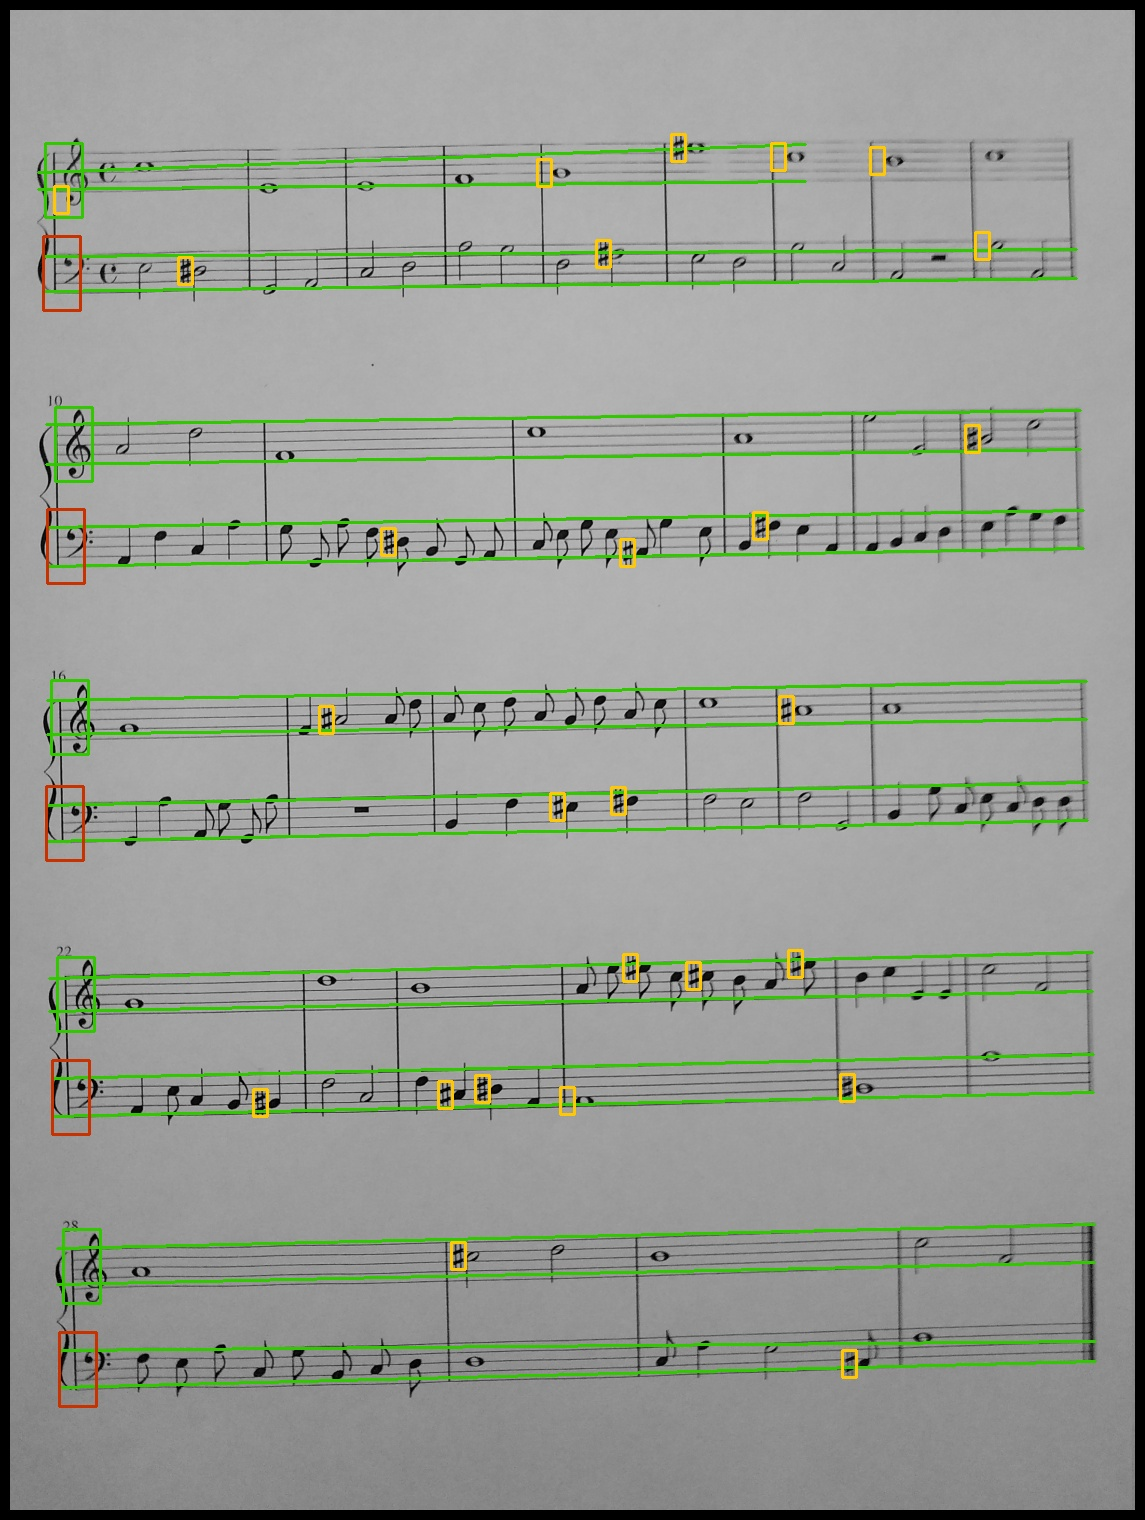
\includegraphics[width=\linewidth]{zdj/step_4.jpg}
				\caption{Krzyżyki}
			\end{subfigure}
			\begin{subfigure}[b]{0.32\linewidth}
				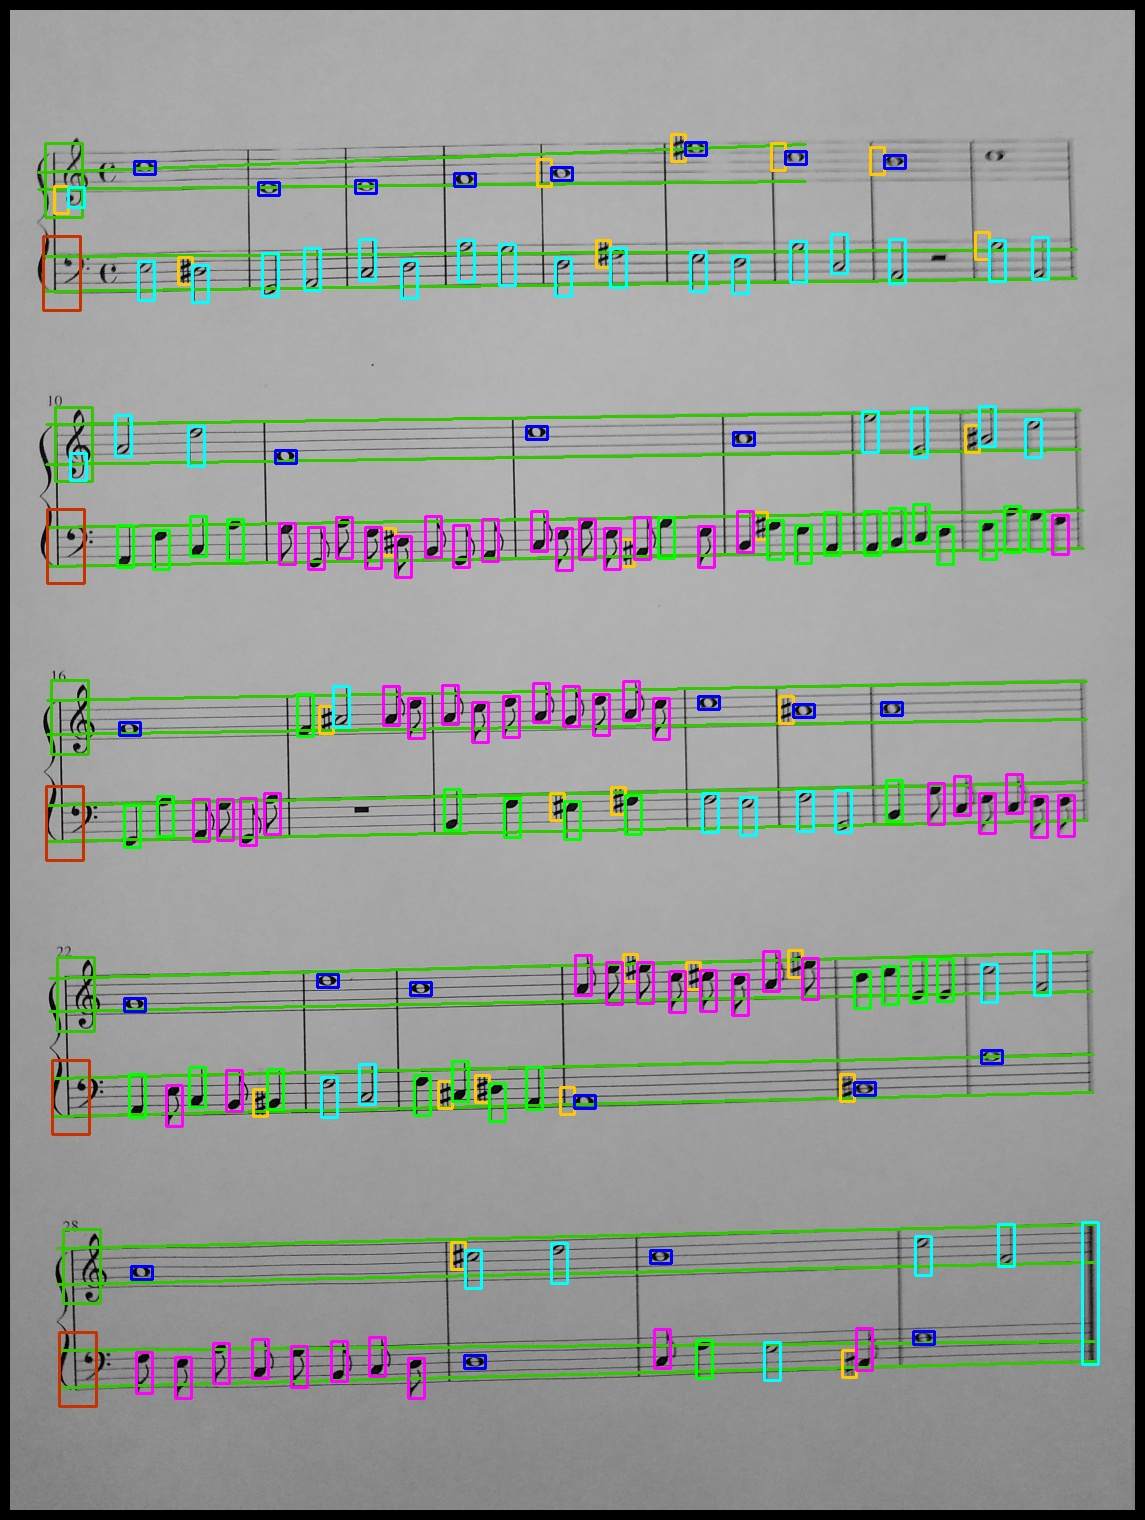
\includegraphics[width=\linewidth]{zdj/step_5.jpg}
				\caption{Efekt końcowy}
			\end{subfigure}
			\begin{subfigure}[b]{0.32\linewidth}
				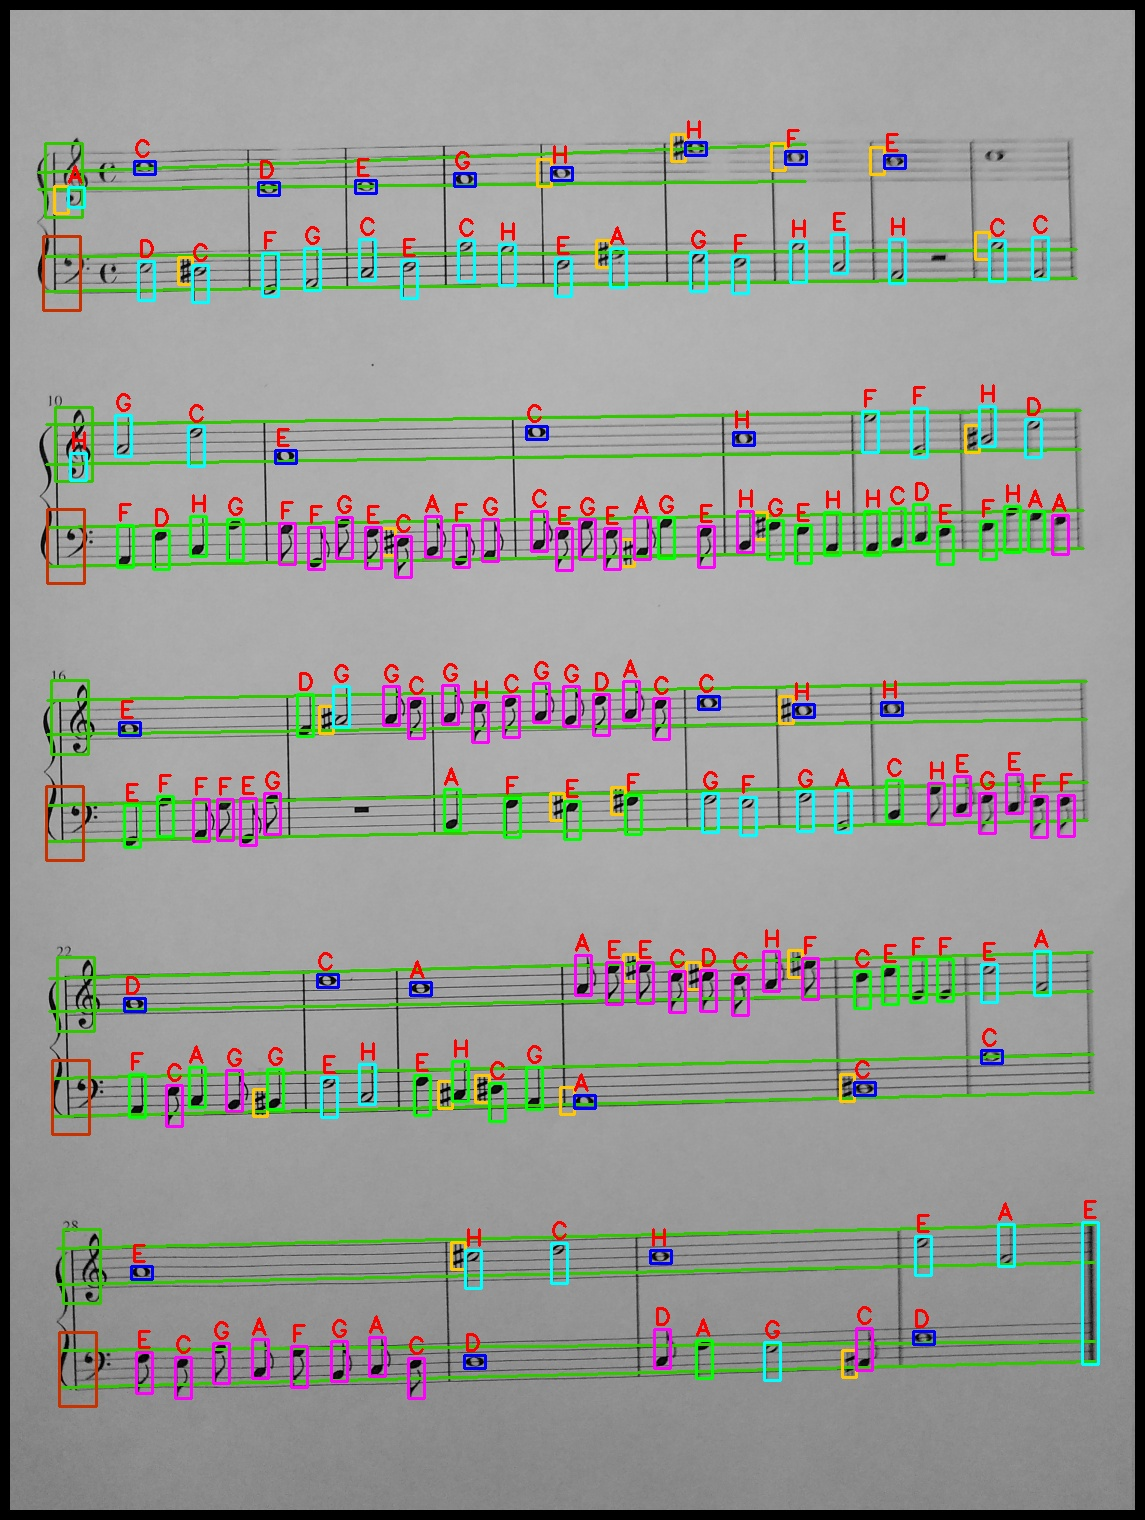
\includegraphics[width=\linewidth]{zdj/step_6.jpg}
				\caption{Efekt końcowy - razem z wysokością nuty}
			\end{subfigure}
			\label{fig:nuty}
			\caption{Etapy detekcji nut}
		\end{figure}
	
	\section{Wyniki}
	
	\section{Posumowanie}
		Detekcja nut najgorzej radzi sobie z nutami pisanymi odręcznie. Dopasowanie wzorców nie sprawdza się tu najlepiej - symbole są różne i mniej stałe. Nawet jeśli nuta zostanie wykryta to jest długość jest źle określana - program interpretuje nie do końca zamalowaną główkę jako otwartą. Pewnym rozwiązaniem mogło by być dodanie dodatkowych wzorców oraz zastosowanie dodatkowych przekształceń obrazu (morfologia, wyrównanie histogramu). Znajdowanie wysokości nut również nie działa idealnie jeśli linie nie są dokładnie równoległe do krawędzi obrazka lub nie są idealnie określone. Zamiast średniej można by zastosować liniową interpolację między współrzędnymi. Wykrywanie nut nie działa idealnie przy przekształceniu perspektywicznym - wzorce mają jeden rozmiar dla całej pięciolinii. Można by spróbować podzielić kartkę na pojedyncze pięciolinie i stosować wzorce na tych pięcioliniach. Problematyczne są także przypadki gdy kartka zostanie obrócona tak, że klucze są po prawej stronie - przy rotacji nie jest uwzględnione położenie kluczy.

\end{document}

